\chapter{Diffusion Limit Results}
\label{Diffusion Limit Results}

The following chapter approaches the issue of complexity of Metropolis-Hastings~(MH) methods for a class of target distributions obtained by a change of measure from a Gaussian measure on an infinite dimensional Hilbert space. This Hilbert setting is widely used in applications as diffusion bridges and Bayesian inverse problems, see Chapter~\ref{Application}. Mattingly, Pillai and Stuart~\autocite{Mattingly2010} and Pillai, Stuart and Thi\'{e}ry~\autocite{Pillai2012} proved that under certain conditions on the regularity of the change of measure and the decay of eigenvalues of the Gaussian covariance operator, a diffusion limit process exists for a suitable scaled version of the MH Markov chain. Hence, according to the research programm initiated by Roberts and coworkers in the pair of papers~\autocite{Roberts1997, Roberts1998} and presented in Chapter~\ref{CC:Optimality and Diffusion Limits}, a computational complexity of $\mathcal{O}(N)$ for the Random Walk Metropolis~(RWM) (introduced in Chapter~\ref{MH-RWM}) and of $\mathcal{O}(N^{1/3})$ for the Metropolis Adjusted Langevin Algorithm~(MALA) (introduced in Chapter~\ref{MH-MALA}) is achieved with dimension~$N$ going to infinity.

This elaboration follows the structure of the the two main references of Mattingly, Pillai and Stuart~\autocite{Mattingly2010} and Pillai, Stuart and Thi\'{e}ry~\autocite{Pillai2012}. Most statements and proofs are taken from these two papers. Since it is our goal to point out a common structure in this two proofs to restate the two main diffusion limit results as one theorem, we will refer to the original papers~\autocite{Mattingly2010, Pillai2012} for several technical estimates.

In Chapter~\ref{sec:DLR-Preliminaries} we define precisely the setting in which the diffusion limit result holds. In Chapter~\ref{sec:DLR-Main theorem} we state the main theorem for RWM and MALA simultaneously and explain it. Chapter~\ref{sec:DLR-Proof} contains the proof of the main theorem, postponing the proof of a number of key technical estimates to Chapter~\ref{sec:DLR-Estimates}.


\subsubsection{Motivation}

We have seen that in applications such as Bayesian approach to inverse problems and conditioned diffusions (see Chapter~\ref{Application}), the target measure of interest, $\pi$, is defined on an infinite dimensional real separable Hilbert space~$\mathcal{H}$. In the case of Gaussian priors (inverse problems) or additive noise (diffusions), $\pi$ is absolutely continuous with respect to a Gaussian reference measure~$\pi_0$ on $\mathcal{H}$ with mean zero and covariance operator~$\mathcal{C}$. The Radon-Nikodym derivative is assumed to have the form
\begin{equation}
\label{DLR-Radon Nikodym derivative}
 \frac{d \pi}{d \pi_0}(x) = M_{\Psi} \exp (- \Psi(x))
\end{equation}
for a real-valued $\pi_0$-measurable functional~$\Psi$ on the Hilbert space and $M_{\Psi}$ is a normalizing constant. This infinite dimensional framework for target measures~$\pi$ of the form~(\ref{DLR-Radon Nikodym derivative}) introduces an inherent mathematical structure  making it conceivable to derive a diffusion limit result for this class of target measures. We highlight two aspects of this mathematical structure. 

First, the theory of Gaussian measures on infinite dimensional Hilbert spaces~$\mathcal{H}$ introduces the possibility to represent~$\mathcal{H}$ via an orthonormal basis of eigenvectors of~$\mathcal{C}$ with~$\mathcal{C}$ as the convariance operator of the Gaussian measure. This representation combined with the Karhunen-Lo\`{e}ve expansion allows us to express any element of~$\mathcal{H}$ distributed according to the reference measure~$\pi_0$ as a possible infinite sum of independent Gaussian random variables. Under certain regularity conditions on~$\Psi$, this subtle product structure is transfered to the target measure corresponding to the change of measure represented by~$\Psi$. This Gaussian embedding is the is the main reason for the working approximation estimates in Chapter~\ref{sec:DLR-Estimates}.

The second aspect of this inherent mathematical structure is the existence of a putative limit diffusion process. In order to prove a limit result as desired, a diffusion candidate is needed, i.e. a diffusion process which is invariant with respect to~$\pi$. In the abstract infinite dimensional Hilbert space setting, linear stochastic partial differential equations~(SPDE) are well understood, e.g. \autocite{DaPrato1992, Hairer2005, Hairer2007}. In the case of linear SPDEs  of the form
\begin{equation}
 dx =  \mathcal{A} x dt + \sqrt{2} \, d \mathcal{W}(t) \qquad x(0)  =0,
\end{equation}
where $ \mathcal{W}(t) $ is a cylindrical Wiener process in $\mathcal{H}$ and $\mathcal{A}$ a suitable linear operator on~$\mathcal{H}$, the invariant distribution is the Gaussian measure~$ \nu = \mathcal{N}(0, -\mathcal{A}^{-1})$ on $\mathcal{H}$. As usual in the theory of (S)PDEs, the linear case is a jumping-off point to the nonlinear equations, just as in this situation. The preconditioned semilinear SPDE is of the form
\begin{equation}
\label{DLR- preconditioned semilinear SPDE - langevin}
 dx = \mathcal{G} (\mathcal{A}x + F(x))dt + \sqrt{2}\mathcal{G}^{1/2} d\mathcal{W}(t), \qquad x(0) = x_0,
\end{equation}
where $\mathcal{A}$ and $\mathcal{W}(t)$ are defined as above and $F: \mathcal{H} \to \mathcal{H}$ is a Fr\'{e}chet differentiable nonlinearity or drift and $\mathcal{G}$ is a self-adjoint, positive linear operator on $\mathcal{H}$, the so-called preconditioner. For further details, we refer to \autocite{Hairer2005, Hairer2007}. This type of SPDE may be viewed as an infinite dimensional analogue of the Langevin equation used in finite dimensions. Accordingly, we will call these SPDEs given by Equation~(\ref{DLR- preconditioned semilinear SPDE - langevin}) \textit{Langevin equations}. Under the assumption that $F = \nabla U$ for a  Fr\'{e}chet differentiable function $U: \mathcal{H} \to \mathbb{R}$ and some regularity conditions on the linear operators~$\mathcal{A}$ and $\mathcal{G}$, the invariant distribution for the Langevin equation defined in Equation~(\ref{DLR- preconditioned semilinear SPDE - langevin}) is given by 
\begin{equation}
 d \eta (x) = M \, e^{U(x)} \, d \nu (x)
\end{equation}
with $\nu = \mathcal{N}(0, - \mathcal{A}^{-1})$. Taking $U = - \Psi$, $\mathcal{G}= \mathcal{C}$ and $\mathcal{A}= - \mathcal{C}^{-1}$, which is well-defined in the case of $\mathcal{C}$ being a covariance operator as considered above, we obtain a $ \mathcal{H} $-valued SDE with the form
\begin{equation}
\label{DLR-limit diffusion candidate}
 dz = - ( z + \mathcal{C} \nabla \Psi (z) ) dt + \sqrt{2} \mathcal{C}^{1/2} d \mathcal{W}(t), \quad z(0) = z_0,
\end{equation}
where $ \mathcal{W}(t) $ is a cylindrical Wiener process in $\mathcal{H}$ and the invariant measure is of the form of $\pi$ as given in Equation~(\ref{DLR-Radon Nikodym derivative}). Moreover, it is shown, that Equation~(\ref{DLR- preconditioned semilinear SPDE - langevin}) has a unique strong and continuous solution. Thus, we have a natural candidate for the infinite dimensional limit diffusion process~\autocite[Theorem 3.6]{Hairer2007}.
\newline

In this setup, our perspective is to apply MCMC methods to finite approximations of the measure~$\pi$ found by projecting onto the first $N$ eigenfunctions of the covariance operator~$\mathcal{C}$ of the Gaussian reference measure~$\pi_0$. These projections allow us to hope for a consistent definition of the finite dimensional approximations. In the following section, we will define this setting rigorously so that we will be enabled to define the RWM- and MALA-type algorithms and so that we will be able to state the diffusion limit result precisely.


\section{Hilbert Space Setting, Assumptions, Projections - Preliminaries}
\label{sec:DLR-Preliminaries}

This section is devoted to stating the setting of the main theorem. As suggested in Chapter~\ref{Application}, the considered setting is complex, and we develop it in a step-by-step fashion. We first introduce the Gaussian reference measure~$\pi_0$ and the change of measure which induces a genuinely nonproduct structure. We then describe a finite dimensional approximation of the measure, enabling us to define a RWM- and MALA-type algorithm.

The structure and most definitions are taken from~\autocite[Section 2]{Pillai2012}. At some passages, we amended it. References for this additonal work will be explicitely given in the text.

\subsubsection{Gaussian Reference Measure}

Let $\mathcal{H}$ be a separable Hilbert space of real-valued functions with inner-product denoted by $\langle \cdot, \cdot \rangle$ and associated norm $\|x\|^2 = \langle x, x \rangle$. Consider a (non-degenrated) Gaussian measure~$\pi_0$ on $(\mathcal{H}, \|\cdot\|)$ with covariance operator~$\mathcal{C}$. According to the general theory of Gaussian measures~\autocite[Chapter I]{DaPrato1992}, $\mathcal{C}$ is a self-adjoint and positive trace class operator on $\mathcal{H}$. Although the concept of Gaussian measures on (infinite dimensional) Hilbert spaces should be familiar to the reader, we briefly recall the definitions of the mean and the covariance of Gaussian measures in Hilbert spaces and the definition of \textit{trace class} operators, since this point is crucial for the understanding.

We start with the definition of Gaussian measures on Hilbert spaces, taken from~\autocite[Section 2.3.2]{DaPrato1992}.

\begin{defin}
\label{DLR-Setting: Definition Gaussian measure}
 Let $(\mathcal{H}, \|\cdot\|)$ be a Hilbert space with inner-product denoted by $\langle \cdot, \cdot \rangle$, a probability measure~$\mu$ on $\mathcal{H}$ is called Gaussian if for arbitrary $y \in \mathcal{H}$ there exist $a \in \mathbb{R}^1, q \geq 0$, such that,
 \begin{equation*}
  \mu \{ x \in \mathcal{H}: \langle y, x \rangle \in D \} = \mathcal{N}(a, q) (D), \qquad D \in \mathcal{B}(\mathbb{R}^1).
 \end{equation*}
\end{defin}

 In particular, if $\mu$ is Gaussian, then there exist an element $m \in \mathcal{H}$ and a self-adjoint, positive and continuous operator $\mathcal{C}$ such that:
 \begin{align}
  \int_{\mathcal{H}} \langle y, x \rangle \mu (dx) = \langle m, y \rangle, \qquad \forall y \in \mathcal{H}, \\
  \int_{\mathcal{H}} \langle y, x - m \rangle \langle z, x - m \rangle \mu (dx) = \langle \mathcal{C}y, z \rangle, \qquad \forall y, z \in \mathcal{H}.
 \end{align}
The element $m \in \mathcal{H}$ is called the \textit{mean} and $\mathcal{C}$ the \textit{covariance} operator of $\mu$. Moreover, the characteristic function of $\mu$ is given by 
\begin{equation*}
 \widehat{\mu} (h) := \int_{\mathcal{H}} e^{i \langle h, x \rangle} \mu(dx) = e^{i \langle h, m \rangle - \tfrac{1}{2} \langle \mathcal{C} h, h \rangle}, \qquad h \in \mathcal{H}.
\end{equation*}
It is therefore uniquely determined by $m$ and $\mathcal{C}$ and is denoted by $ \mathcal{N}(m, \mathcal{C})$.

The covariance operator~$\mathcal{C}$ has some further properties, it turns out that it is a trace class operator~\autocite[Proposition 2.15]{DaPrato1992}.

\begin{defin}\autocite[Section 1.1]{DaPrato2002}
\label{DLR-Setting: Definition trace class}
 Let $\mathcal{H}$ be a separable Hilbert space with inner-product and norm denoted by $\langle \cdot, \cdot \rangle$ and $\| \cdot \|$. A bounded linear operator $\mathcal{A}$ on $\mathcal{H}$ is said to be of trace class if there exist two sequences~$\{ a_j \}, \{ b_j \}$ in $\mathcal{H}$ such that
 \begin{equation*}
  \mathcal{A}x := \sum_{j \in I} \langle x, a_j \rangle b_j, \qquad x \in \mathcal{H},
 \end{equation*}
 and
 \begin{equation*}
  \sum_{j \in I} \| a_j \| \| b_j \| < + \infty.
 \end{equation*}
 If an operator~$\mathcal{A}$ is of trace class then its trace, $\text{Tr}_{\mathcal{H}}\mathcal{A}$, is defined by the formula
 \begin{equation}
  \text{Tr}_{\mathcal{H}}(\mathcal{A}) := \sum_{j \in I} \langle e_j, \mathcal{A} e_j \rangle,
 \end{equation}
 where~$\{ e_j : j \in I \}$  is an orthonormal and complete basis on $\mathcal{H}$.

\end{defin}

Trace class operators have some useful properties. First, note that the definition of the trace is independent of the orthonormal basis~\autocite[Proposition C.1]{DaPrato1992}. More important is the second fact: if $\mathcal{A}$ is a positive and self-adjoint trace class operator (like the covariance operator~$\mathcal{C}$) then it is diagonizable (being a bounded trace class operator implies that it is compact): there is an orthonormal basis~$\{ e_j : j \in I \}$ for $\mathcal{H}$ consisting of eigenvectors of $\mathcal{A}$ such that $\mathcal{A} e_j = \eta_j e_j $ and $\eta_j > 0, \sum_{j \in I} \eta_j < + \infty$; see~\autocite[Lemma 6.32]{Dashti2014} and~\autocite[Proposition 3.15]{Hairer2009}. Thus, a given Gaussian measure introduces a lot of structure in form of a complete eigenbasis to the underlying Hilbert space. This subtle structure is essential for proving the diffusion limit result.


Therefore, let $\{ \varphi_j, \lambda_j^2 \}_{j \geq 1}$ be the eigenfunctions and eigenvalues of the covariance operator~$\mathcal{C}$ of the Gaussian measure~$\pi_0$:
\begin{equation}
\label{DLR-Setting: Eigefunctions}
 \mathcal{C} \varphi_j = \lambda_j^2 \varphi_j, \qquad j \geq 1. 
\end{equation}
We assume a normalization under which $\{ \varphi_j \}_{j \geq 1}$ forms a complete orthonormal basis in the Hilbert space $\mathcal{H}$, which we refer to as the Karhunen-Lo\`{e}ve basis. Henceforth, we assume that the eigenvalues are arranged in decreasing order and note $\lambda_j > 0$. Any function~$x \in \mathcal{H}$ can be represented in the orthonormal eigenbasis of $\mathcal{C}$ via the expansion
\begin{equation}
\label{DLR-Setting: karhunen-loeve representation}
 x = \sum_{j = 0}^{\infty} x_j \varphi_j, \qquad x_j := \langle x, \varphi_j \rangle.
\end{equation}
It will often be helpful, to identify the function~$x$ with its coordinates~$\{ x_j \}_{j=1}^{\infty} \in l^2$ in the eigenbasis and vice versa, where $l^2$ denotes the sequence space of square summable sequences. By the Karhunen-L\`{e}ve or white noise expansion~\autocite[Section 2.2.3]{DaPrato1992}, a realization~$x$ from the Gaussian reference measure~$\pi_0$ can be expressed by allowing the coordinates~$\{x_j\}_{j \geq 1}$ to be independent Gaussian random variables distributed according $\mathcal{N}(0, \lambda_j^2)$ in $\mathbb{R}$. Thus, the Gaussian reference measure~$\pi_0$ possesses a product structure in the coordinate-representation.


Frequently in applications, the functional~$\Psi$ in Equation~(\ref{DLR-Radon Nikodym derivative}) may not be well-defined on all of $\mathcal{H}$, in the sense that some regularity conditions on $\Psi$ hold only on a subset $\mathcal{H}^r \subset \mathcal{H}$ for some exponent~$r > 0$. For instance, if $ \mathcal{H}= L^2([0,1]) $, the functional~$\Psi$ might only act well on continuous functions, in which case it is natural to define~$\Psi$ on some Sobolev-like space~$\mathcal{H}^r([0,1])$ for $r > \tfrac{1}{2}$. In such a situation, we can revert to  Sobolev embeddings~\autocite[Theorem 6.3]{Hairer2009}.


To follow this purpose, we now define Sobolev-like spaces~$\mathcal{H}^r , r \in \mathbb{R}$, also called Hilbert scale spaces. Given a Hilbert space~$ (\mathcal{H}, \langle \cdot, \cdot \rangle, \| \cdot \|) $ of real-valued functions, and  $\{ \varphi_j \}_{j \geq 1}$ an orthonormal basis for~$\mathcal{H}$, for any $x \in \mathcal{H}$ the representation in Equation~(\ref{DLR-Setting: karhunen-loeve representation}) holds. Thus, we can define
\begin{equation}
 \mathcal{H}^r := \left\{ x \in \mathcal{H}: \| x \|_r^2 < \infty \right\}
\end{equation}
where $r \in \mathbb{R}$ and, for $ x_j = \langle x, \varphi_j \rangle $,
\begin{equation}
\label{DLR-Setting: H^r norm}
 \| x \|_r^2 := \sum_{j=1}^{\infty} j^{2r} x_j^2.
\end{equation}
In fact $\mathcal{H}^r$ is a Hilbert space: for $ y_j = \langle y, \varphi_j \rangle $ we define the inner-product
\begin{equation}
 \langle x, y \rangle_{r} := \sum_{j=1}^{\infty} j^{2r} x_j y_j.
\end{equation}
For any $r>0$, the Hilbert space~$ (\mathcal{H}^r, \langle \cdot, \cdot \rangle_r, \| \cdot \|_r) $ is a subset of the original Hilbert space~$\mathcal{H}$; for $r<0$ the spaces are defined by duality and are supersets of $\mathcal{H}$. These spaces are again separable Hilbert spaces for any $r \in \mathbb{R}$ as they are linked to the sequence space~$l^2$ with weights~$\omega_j = j^{2r}$ which are separable~\autocite[Section 6.1.3]{Dashti2014}.

For $x,y \in \mathcal{H}^r$, the outer product operator in $\mathcal{H}^r$ is the operator~$ x \otimes_{\mathcal{H}^r} y : \mathcal{H}^r \to \mathcal{H}^r $ defined by $ (x \otimes_{\mathcal{H}^r} y) z := \langle y, z \rangle_r x $ for every $ z \in \mathcal{H}^r$. Moreover, we want to transfer the covariance operator~$\mathcal{C}$ to $\mathcal{H}^r$. For $r \in \mathbb{R}$, let $B_r: \mathcal{H} \to \mathcal{H}$ denote the operator which is diagonal in the basis~$\{ \varphi_j \}_{j \geq 1}$ with diagonal entries~$j^{2r}$ so that $B_r^{1/2} \varphi_j = j^{r} \varphi_j$. The operator~$B_r$ lets us alternate between $\mathcal{H}$ and $\mathcal{H}^r$ by the following identity $ \langle x, y \rangle_r = \langle B_r^{1/2} x, B_r^{1/2} y \rangle$. Since $B_r^{-1/2} $ is an isometry, the family~$\{ \phi_j \}_{j \geq 1}$ forms a complete orthonormal basis for~$\mathcal{H}^r$ with $ \phi_j(r) := B_r^{-1/2} \varphi_j$. Similar to Definition~\ref{DLR-Setting: Definition trace class}, we can define the trace on $\mathcal{H}^r$ by
\begin{equation}
 \label{DLR-Setting: Trace on H^s}
 \text{Tr}_{\mathcal{H}^r}(\mathcal{A}) := \sum_{j=1}^{\infty} \langle (B_r^{-1/2}\varphi_j ), \mathcal{A}( B_r^{-1/2}\varphi_j) \rangle_r.
\end{equation}
For a positive and bounded operator~$\mathcal{A}$ it suffices to show that the trace~$\text{Tr}_{\mathcal{H}^r}(\mathcal{A})$ is finite, to conclude that $\mathcal{A}$ is of trace class~\autocite[Proposition C.3]{DaPrato1992}. We define the linear operator~$\mathcal{C}_r := B_r^{1/2} \mathcal{C} B_r^{1/2} $ with $ \text{Tr}_{\mathcal{H}^r}(\mathcal{C}_r) = \sum_{j=0}^{\infty} \lambda_j^2 j^{2r}$. Under the condition
\begin{equation}
\label{DLR-Setting: Gaussian measure on H^r condition}
 \text{Tr}_{\mathcal{H}^r}(\mathcal{C}_r) < \infty,
\end{equation}
we can conclude that the positive and self-adjoint operator~$\mathcal{C}_r$ is of trace class and therefore a Gaussian measure on~$\mathcal{H}^r$ with covariance operator~$\mathcal{C}_r$ exists~\autocite[Proposition 2.18]{DaPrato1992}. This Gaussian measure on~$\mathcal{H}^r$ is induced by the reference measure~$\pi_0$ on~$\mathcal{H}$, and $ \pi_0(\mathcal{H}^r ) =1$, if the condition in Equation~(\ref{DLR-Setting: Gaussian measure on H^r condition}) holds. Indeed, we claim that $\mathcal{C}_r$ is the covariance operator of the Gaussian measure~$\pi_0$ on $\mathcal{H}^r$ by verifying the definitions; see~\autocite[Chapter 2.3]{DaPrato1992} for an introduction to Gaussian measures on Hilbert spaces.

\begin{proposition}
\label{DLR-Setting: Proposition Gaussian measure}
 Let $\xi \stackrel{D}{\sim} \pi_0$, then $\mathbb{E} [\langle \xi, u \rangle_r \langle \xi , v \rangle_r ] = \langle u , \mathcal{C}_r v \rangle_r$ for any functions $u,v \in \mathcal{H}^r$. Similarly, $\mathbb{E} [\langle \xi, u \rangle_r  ] = 0$ for any function $u \in \mathcal{H}^r$.
\end{proposition}

\begin{proof}
 Let $\xi \stackrel{D}{\sim} \pi_0$, then by using the definition of the covariance operator~$\mathcal{C}$ and of the inner-product $\langle \cdot, \cdot \rangle_r$, we conclude,
 \begin{align*}
  \int_{\mathcal{H}} \langle \xi, u \rangle_r \langle \xi , v \rangle_r \; \pi_0 (d\xi) & \; = \langle \mathcal{C} B_r u , B_r v \rangle \\
  & \; = \langle B_r^{1/2} \mathcal{C} B_r u , B_r^{1/2} v \rangle \\
  & \; = \langle  B_r u , \mathcal{C}_r v \rangle \\	
  & \; = \langle  B_r^{1/2} u , B_r^{1/2} \mathcal{C}_r v \rangle = \langle u, \mathcal{C}_r v \rangle_r.
 \end{align*}
 We used the self-adjointness of $\mathcal{C}$ and $B_r$. Similarly, we can conclude for the mean.

\end{proof}

Additionally, we claim that if $\text{Tr}_{\mathcal{H}^r}(\mathcal{C}_r)$ is finite, $\pi_0$ has full support on the subspace $\mathcal{H}^r$.

\begin{proposition}
\label{DLR-Setting: Proposition Full support}
 Under the condtion given in Equation~(\ref{DLR-Setting: Gaussian measure on H^r condition}), $\pi_0 $-almost every function~$x \in \mathcal{H}$ belongs to $\mathcal{H}^r$.
\end{proposition}

\begin{proof}
 Let $x \in \mathcal{H}$, then by monotone convergence and using the definition of the covariance operator~$\mathcal{C}$ of the Gaussian measure~$\pi_0$, we conclude
 \begin{align*}
  \int_{\mathcal{H}} \| x \|_r^2 \; \pi_0 (dx) & \; = \int_{\mathcal{H}} \sum_{j=1}^{\infty} x_j j^{2r} \; \pi_0 (dx)  \\
  & \; = \sum_{j=1}^{\infty} j^{2r} ( \int_{\mathcal{H}}  \langle x, \varphi_j \rangle^2  \; \pi_0 (dx) )  \\
  & \; = \sum_{j=1}^{\infty} j^{2r} (   \langle \mathcal{C} \varphi_j, \varphi_j \rangle   )    \\
  & \; = \sum_{j=1}^{\infty} j^{2r} \lambda_j^2 < \infty.
 \end{align*}
 The first and second identy follows from the representation of the $\mathcal{H}^r$-norm in Equation~(\ref{DLR-Setting: H^r norm}) and the Karhunen-Lo\'{e}ve representation in Equation~(\ref{DLR-Setting: karhunen-loeve representation}). As stated in Equation~(\ref{DLR-Setting: Eigefunctions}), $\{  \varphi_j \}_{j \geq 1}$ are eigenfunctions of $\mathcal{C}$ and $\text{Tr}_{\mathcal{H}^r}(\mathcal{C}_r) < \infty$ as assumed. Thus, we finish the proof.

\end{proof}

Hence, we alternate between both Gaussian measures~$\mathcal{N}(0, \mathcal{C})$ on $\mathcal{H}$ and $\mathcal{N}(0, \mathcal{C}_r)$ on $\mathcal{H}^r$, for those $r$ for which $\text{Tr}_{\mathcal{H}^r}(\mathcal{C}_r)$ is finite. Moreover, there will be a subtle change in the choice of the basis. In the next subsection we will fix an exponent~$r>0$ and denote it by~$s$ such that $\text{Tr}_{\mathcal{H}^s}(\mathcal{C}_s) < \infty$. By doing this, we will completely switch to this Sobolev space~$\mathcal{H}^s$, in particular we will considering the basis~$\phi_j(s) = \phi_j := B^{-1/2}_s \varphi_j$. Thus, every coordinate of an object of~$\mathcal{H}^s$ will be given with respect to this basis. To avoid irritation, we recall some definitions and facts due to this basis change. The inner product on $\mathcal{H}^s$ reads
\begin{equation}
  \langle x, y \rangle_s = \sum_{j=1}^{\infty} x_j y_j \quad \text{ for } x_j = \langle x, \phi_j\rangle_s
\end{equation}
and the norm on $\mathcal{H}^s$ is given by
\begin{equation}
  \| x \|_s^2 = \sum_{j=1}^{\infty} x_j^2 \quad \text{ for } x_j = \langle x, \phi_j\rangle_s.
\end{equation}
On $\mathcal{H}^s$ we will consider the positive, self-adjoint trace-class operator~$\mathcal{C}_s$ with the eigenbasis~$\{ \phi_j,  \lambda_j^2 j^{2s} \}_{j \geq 1}$ of the Gaussian measure~$\pi_0$ projected to $\mathcal{H}^s$: for $j \geq 1$
\begin{equation}
\label{DLR-Setting: Definition Eigefunctions of C_s}
   \mathcal{C}_s \phi_j = B_s^{1/2} \mathcal{C}B^{1/2}_sB^{-1/2}_s \varphi_j  =  \lambda_j^2 j^s \varphi_j = ( \lambda_j^2 j^{2s}) \phi_j.
\end{equation}

\begin{rem}
  \label{DLR-Remark Change of basis}
  In comparison to~\autocite{Mattingly2010, Pillai2012}, we change the notation as we will consequently use the eigenbasis~$\{ \phi_j,  \lambda_j^2 j^{2s} \}_{j \geq 1}$ of $\mathcal{C}_s$ on $\mathcal{H}^s$. This basis change do not disrupt the results given in the original papers but it allows us to work with the operator~$\mathcal{C}_s$ instead of $\mathcal{C}$ such that we can state our main result in a consitent fashion. As we will refer to these original works for some  proofs, we want to emphasize that all calculations with the operator~$\mathcal{C}$ in its eigenbasis~$\{ \varphi_j,  \lambda_j^2 \}_{j \geq 1}$ do not change if one considers the operator~$\mathcal{C}_s$ with its eigenbasis~$\{ \phi_j,  \lambda_j^2 j^{2s} \}_{j \geq 1}$ instead. Indeed, we have
  \begin{equation}
    \begin{split}
      \| \mathcal{C}x \|_s^2 & = \sum_{j=1}^{\infty} j^{2s} \lambda_j^2 \left(x_j^2 (\mathcal{H})\right), \\
       \| \mathcal{C}_sx \|_s^2 & = \sum_{j=1}^{\infty} j^{2s} \lambda_j^2 \left(x_j^2(\mathcal{H}^s)\right),\\
    \end{split}
  \end{equation}
 where we distinguished between the two coordinates~$x_j^2 (\mathcal{H}) $ with respect to the eigenbasis of~$\mathcal{C}$ and $x_j^2(\mathcal{H}^s)$ with respect to the eigenbasis of $\mathcal{C}_s$. Furthermore, we identify the dual space of~$\mathcal{H}^s$ denoted by $(\mathcal{H}^s)^*$ with $\mathcal{H}^s$ as it is a Hilbert space.
\end{rem}




\subsubsection{Change of Measure}

The target measure of interest, $\pi$, from which we want to sample is defined through the change of measure defined in Equation~(\ref{DLR-Radon Nikodym derivative}) via the functional~$\Psi$. As the measure~$\pi_0$ has full support on~$\mathcal{H}^s$, if $\text{Tr}_{\mathcal{H}^r}(\mathcal{C}_r) < \infty$, the functional~$\Psi$ needs only to be defined on $\mathcal{H}^s$ such that the Radon-Nikodym derivative of the change of measure is well-defined.

We will give assumptions on the decay of eigenvalues of the covariance operator~$\mathcal{C}$ of~$\pi_0$ in order to ensure the existence of a real number~$s > 0$ such that Equation~(\ref{DLR-Setting: Gaussian measure on H^r condition}) is fulfilled and $\pi_0$ has full support on $\mathcal{H}^s$. Furthermore, we impose regularity conditions on the functional~$\Psi$. These assumptions shall ensure that the target measure~$\pi$ is not too different from the Gaussian measure~$\pi_0$ such that we can ascribe further properties of the Gaussian measure~$\pi_0$ to $\pi$~(see Lemma~\ref{DLR-Proof: Lemma Convergence of pi^N to pi} and Remark~\ref{DLR: Remark Fernique's theorem}). These assumptions can be summarized as follows: the functional~$\Psi$ has to be quadratically bounded, with first derivative linearly bounded, and the second derivative globally bounded. By using the identification of the dual spaces for Hilbert spaces, we can formulate our assumptions precisely. See~\autocite[Assumption 2.1]{Pillai2012} for further details.

\begin{assum}
 \label{DLR-Setting: Assumptions on C and Psi}
 The covariance operator $\mathcal{C}$ and the functional~$\Psi$ satisfy the following:
 \begin{enumerate} 
  \item[(1)] \textit{Decay of eigenvalues~$\lambda_j^2$ of $\mathcal{C}$: } There is an exponent~$\kappa > \tfrac{1}{2}$ such that
 \begin{equation}
 \label{DLR-Seeting: Assumption on decay of eigenvalues}
  \lambda_j \asymp j^{- \kappa}.
 \end{equation}
 \item[(2)] \textit{Assumptions on $\Psi$: } There exist constants $M_i \in \mathbb{R}, i \leq 4$, and $s \in [0, \kappa - 1/2)$ such that for all $x \in \mathcal{H}^s$ the functional~$\Psi: \mathcal{H}^s \to \mathbb{R}$ satisfies
 \begin{align}
 \label{DLR-Setting: Assumption on Psi 1}
  M_1 & \; \leq \Psi(x) \leq M_2 (1+ \| x \|_s^2), \\
  \label{DLR-Setting: Assumption on Psi 2}
  \| \nabla \Psi (x) \|_{-s} & \; \leq M_3 (1+\| x\|_s), \\
  \label{DLR-Setting: Assumption on Psi 3}
  \| \partial^2 \Psi (x) \|_{\mathcal{L}(\mathcal{H}^s, \mathcal{H}^{-s})} & \; \leq M_4.
 \end{align}
 \end{enumerate}
\end{assum}

Here we used the following notation. Two sequences $\{\alpha_n\}$ and $\{\beta_n\}$ satisfy $\alpha_n \lesssim  \beta_n$ if there exists a constant~$M>0$ such that $\alpha_n \leq M \; \beta_n$ for all $n \leq 0$. The notation~$\alpha_n \asymp \beta_n$ means that $\alpha_n \lesssim  \beta_n $ and $ \beta_n \lesssim  \alpha_n$~\autocite{Pillai2012}.

\begin{rem}
 The growth condition~$\kappa > \tfrac{1}{2}$ ensures that the covariance operator~$\mathcal{C}$ of~$\pi_0$ is of trace class as $\text{Tr}_{\mathcal{H}}(\mathcal{C}) = \sum_{j=1}^{\infty} \lambda_j^2$. In fact, the condition on the trace of~$\mathcal{C}_r$ in Equation~(\ref{DLR-Setting: Gaussian measure on H^r condition}) is satistied if and only if $r < \kappa - \tfrac{1}{2}$. Indeed, under Assumption~\ref{DLR-Setting: Assumptions on C and Psi}, we calculate
 \begin{equation*}
  \text{Tr}_{\mathcal{H}^r}(\mathcal{C}_r) = \sum_{j=1}^{\infty} \lambda_j^2 j^{2r}  \asymp \sum_{j=1}^{\infty} j^{2(r-\kappa)} < \infty, \qquad \text{for } \; r < \kappa - \tfrac{1}{2}.
 \end{equation*}
 We choose now and for the rest of this chapter, $s \in [0, \kappa - \tfrac{1}{2})$. We define the Sobolev space~$\mathcal{H}^s$ and the reference Gaussian measure~$\pi_0$ has full support on~$\mathcal{H}^s$ as the condition in Equation~(\ref{DLR-Setting: Gaussian measure on H^r condition}) is fulfilled. Thus, the Radon-Nikodym derivative of $\pi$ in Equation~(\ref{DLR-Radon Nikodym derivative}) is well-defined with the change of measure~$\Psi$. Indeed, all regularity assumptions on~$\Psi$ given in Assumption~\ref{DLR-Setting: Assumptions on C and Psi} are defined on $\mathcal{H}^s$ a subset of $\mathcal{H}$ with full measure under~$\pi_0$. These assumptions ensure $\Psi$ to be Lipschitz-continuous on $\mathcal{H}^s$ and therefore it is $\pi_0$-measurable. 

\end{rem}


\begin{rem}
  \label{DLR: Assumption on C_s}
  The assumption on the decay of eigenvalues~$\lambda_j^2$ of $\mathcal{C}$ results directly in the decay of eigenvalues~$\lambda_j^2 j^{2s}$ of $\mathcal{C}_s$: There is an exponent~$\kappa > \tfrac{1}{2}$ such that
 \begin{equation}
 \label{DLR-Seeting: Assumption on decay of eigenvalues of C_s}
 \lambda_j j^{s} \asymp j^{s - \kappa}.
 \end{equation}
 As $s < \kappa -\tfrac{1}{2}$, we conclude: $ s -\kappa < - \tfrac{1}{2} $.
\end{rem}



The assumptions given on the decay of eigenvalues of $\mathcal{C}$ given in Equation~(\ref{DLR-Seeting: Assumption on decay of eigenvalues}) implies that the covariance operator~$\mathcal{C}_s$ has a smoothing effect.

\begin{lemma}\autocite[Lemma 3.3]{Mattingly2010}
\label{DLR-Setting: Smoothing effect of C}
 Under Assumption~\ref{DLR-Setting: Assumptions on C and Psi}, it follows that for all~$\alpha \in \mathbb{R}$,
 \begin{equation}
   \| \mathcal{C}_s^{\alpha} x \|_{s} \asymp \| x \|_{2 \alpha (s - \kappa)}, \qquad \text{for } x \in \mathcal{H}^s.
 \end{equation}
 
\end{lemma}

\begin{proof}
 By using the decay of eigenvalues of~$\mathcal{C}_s$, we establish both required inequalities from the definitions of the appropriate norms.
 \begin{equation*}
   \| \mathcal{C}_s^{\alpha} x \|_{s}^2 = \sum_{j=1}^{\infty} (j^{2 s} \lambda_j^2)^{2 \alpha} x_j^2 \asymp  \sum_{j=1}^{\infty} j^{4 \alpha (s - \kappa)} x_j^2 = \| x \|_{ 2 \alpha ( s - \kappa)}^2.
 \end{equation*}

\end{proof}


\subsubsection{Finite Dimensional Approximation}

In order to sample from the target probability distribution~$\pi$, we are interested in its finite dimensional approximations to apply a Metropolis-Hastings method. Therefore, we introduce the vector space spanned by the first~$N$ eigenfunctions of the covariance operator~$\mathcal{C}_s$,
\begin{equation}
 X^N := \text{span} \{ \phi_1, \phi_2, \dots , \phi_N \},
\end{equation}
where $\phi_j$ build the orthonormal basis of~$\mathcal{H}^s$ as mentioned above. Thus, $X^N$ is a subspace of $\mathcal{H}^s$ for $s < \kappa - \tfrac{1}{2}$. In a second step, we define the $N$-dimensional approximations of the funcional~$\Psi$ and of the reference measure~$\pi_0$. To this end, we introduce the orthogonal projection on $X^N$ denoted by $P^N : \mathcal{H}^s \to X^N \subset \mathcal{H}^s$, that is,
\begin{equation}
  \label{DLR: Finite dimensional approximation - definition projection}
 P^N x := \sum_{j=1}^N  x_j \phi_j, \qquad \text{where } x_j := \langle x, \phi_j\rangle_s, \quad x \in \mathcal{H}^s.
\end{equation}
This shows that the $N$-dimensional vector space~$X^N$ is isomorphic to~$\mathbb{R}^N$.

\begin{rem}
 The identification of $X^N$ with $\mathbb{R}^N$ is very useful for the implementation of the Metropolis-Hastings algorithms. In applications, they will be used to simulate the coordinates, which leads to a representation of the functions in the eigenbasis of the covariance operator.
\end{rem}

The functional~$\Psi$ is approximated by the functional~$\Psi^N : X^N \to \mathbb{R}$ defined by
\begin{equation}
\label{DLR-Setting: Definition Psi^N}
 \Psi^N := \Psi \circ P^N.
\end{equation}
The approximation of the reference measure~$\pi_0$ is the Gaussian measure on $X^N$ given by the law of the random variable
\begin{equation*}
 \pi^N_0 \stackrel{D}{\sim} \sum_{j=1}^{N} \lambda_j \xi_j \phi_j = (\mathcal{C}^N_s)^{1/2} \xi^N, 
\end{equation*}
where $\xi^N = \sum_{j=1}^{N} \xi_j \phi_j$ denotes a $N$-dimensional Gaussian in $X^N$ with $\xi_j$ are i.i.d.\,standard Gaussian random variables and  $\mathcal{C}_s^N :=P^N \circ \mathcal{C}_s \circ P^N $. Consequently, we have $\pi_0^N = \mathcal{N}(0, \mathcal{C}_s^N)$ with
\begin{equation*}
 \pi_0^N (x) \varpropto \exp (- \tfrac{1}{2} \langle x, (\mathcal{C}^N_s)^{-1} x \rangle).
\end{equation*}
Finally, one can define the approximation~$\pi^N$ of $\pi$ by the change of probability formula
\begin{equation}
\label{DLR-Setting: Definition of pi^N}
 \frac{d \pi^N}{d \pi_0^N} (x) = M_{\Psi^N} \exp (- \Psi^N (x)).
\end{equation}
The constant~$M_{\Psi^N}$ is chosen such that $\pi^N (\mathcal{H}^s) =1$. As $X^N$ is finite dimensional, there exists a Lebesgue measure on it. Hence on $X^{N}$, the probability distribution $\pi^{N}$ has Lebesgue density equal to
\begin{equation}
\label{DLR-Setting: Definition finite dim target measure pi^N}
 \pi^N (x) \varpropto \exp (-\tfrac{1}{2} \| x \|^2_{\mathcal{C}_s^N} - \Psi^N (x)).
\end{equation}
The Hilbert-Schmidt norm  $ \| \cdot \|_{\mathcal{C}_s^{N}} $ on $X^{N}$ associated to the operator~$\mathcal{C}^N$ is given by the scalar product $ \langle u, v \rangle_{\mathcal{C}_s^{N}} := \langle u, ( \mathcal{C}_s^{N} )^{-1} v \rangle_s $ for all $ u,v \in X^{N} $. Since the eigenvalues of $ \mathcal{C} $ are assumed to be strictly positive, the operator $ \mathcal{C}_s^{N} $ is invertible on $X^{N}$. Under the assumption that the functionals~$\Psi^N$ satisfy the same conditons as $\Psi$ given in Assumption~\ref{DLR-Setting: Assumptions on C and Psi}, it is straight forward to show the the sequence of measures~$\{ \pi^N \}_N$ converges to $\pi$ in the Hellinger metric. See~\autocite[Theorem 2.6]{Cotter2010} and note that due to the regularity assumptions on~$\Psi$, for any $R>0$, there exists a constant $K=K(R)>0$ such that, for all $x\in \mathcal{H}^s$ with $\|x\|_s < R$,
\begin{equation*}
 | \Psi (x) - \Psi^N (x) | \leq K \psi(N) 
\end{equation*}
holds with $\psi(N) := \| \text{Id} - P^N \|_{\mathcal{L}(\mathcal{H}^s, \mathcal{H}^s)} \to 0$ for $N \to \infty$. Hence, the measures~$\{ \pi^N \}_N$ are good candidates for finite dimensional approximations of~$\pi$. Similar to general case in Equation~(\ref{DLR- preconditioned semilinear SPDE - langevin}), there exists a Langevin diffusion on~$\mathcal{H}^s$ defined by
\begin{equation}
 d \tilde{z} = - ( \tilde{z} + \mathcal{C}_s^N \nabla \Psi^N (\tilde{z}) ) dt + \sqrt{2} (\mathcal{C}_s^N)^{1/2} d \mathcal{W}(t), \quad \tilde{z}(0) = \tilde{z}_0,
\end{equation}
which  leaves $ \pi^{N} $ invariant, where $\mathcal{W}(t)$ is a cylindrical Wiener process. We define the drift~$\mu^N: \mathcal{H}^s \to \mathcal{H}^2$ of this SDE to be
\begin{equation}
\label{DLR-Setting: Definition aproximated drift mu^N}
 \mu^N (x) := - \left(  P^N x + \mathcal{C}_s^N \nabla \Psi^N (x)  \right)
\end{equation}
which is $ \mathcal{C}_s^{N} \nabla \log \pi^{N} (x) $, up to an additive constant. This can be seen easily, as $ \tfrac{1}{2}  \nabla \left( \| x \|_{\mathcal{C}_s^N}^2 \right) = (\mathcal{C}_s^N)^{-1} x  $ for $x \in \mathcal{H}^s$. Analogously, we define the drift function~$\mu : \mathcal{H}^s \to \mathcal{H}^s$ by
\begin{equation}
\label{DLR-Setting: Definition drift mu}
 \mu(x) := - (x + \mathcal{C}_s \nabla \Psi (x) ).
\end{equation}
This is the drift of the Langevin diffusion in Equation~(\ref{DLR- preconditioned semilinear SPDE - langevin}) and can informally be seen as  $ \mathcal{C}_s \nabla \log \pi^{N} (x) $, up to an additive constant. In what follows, we will show that the approximated drift~$\mu^N(x)$ converges to $\mu(x)$, see Lemma~\ref{DLR-Proof: Lemma Convergence of pi^N to pi}.

These definitions enable us to summarize various regularity results on the functionals~$\Psi$ and~$\Psi^N$.

\begin{lemma}\autocite[Lemma 2.4]{Pillai2012}
\label{DLR-Seeting: Lemma: Properties of Psi and Psi^N}
 Let the functional~$\Psi$ satisfy Assumption~\ref{DLR-Setting: Assumptions on C and Psi} and consider the functional~$\Psi^N$ defined by Equation~(\ref{DLR-Setting: Definition Psi^N}). The following etsimates hold:
 \begin{enumerate}
  \item[(1)] The functionals~$\Psi^N : \mathcal{H}^s \to \mathbb{R}$ satisfy the same conditions imposed on $\Psi$ given by Equations~(\ref{DLR-Setting: Assumption on Psi 1}), (\ref{DLR-Setting: Assumption on Psi 2}) and~(\ref{DLR-Setting: Assumption on Psi 3}) with a constant independent of~$N$.
  \item[(2)]  The functional~$\Psi: \mathcal{H}^s \to \mathbb{R}$ satisfies a second order Taylor formula. There exists a constant$M_6 >0$ such that
  \begin{equation}
  \label{DLR-Setting: Psi Taylor formula}
   \Psi(y) - \left( \Psi(x) + \langle \nabla \Psi(x), y-x \rangle \right) \leq M_5 \|x-y\|_s^2 \qquad \forall x,y \in \mathcal{H}^s. 
  \end{equation}
  Furthermore, the functionals~$\Psi^N$ also satisfies this estimate with a constant independently of~$N$.
  \item[(3)] The functions~$\nabla \Psi: \mathcal{H}^s \to \mathcal{H}^s$ and $\mathcal{C}_s\nabla \Psi: \mathcal{H}^s \to \mathcal{H}^s$ are globally Lipschitz on $\mathcal{H}^s$: there exists a constant~$M_5>0$ such that
  \begin{equation*}
    \begin{split}
      \|\nabla \Psi (x) - \nabla \Psi (y) \|_s & \; \leq M_6 \|x - y \|_s \qquad \forall x,y \in \mathcal{H}^s, \\
       \| \mathcal{C}_s\nabla \Psi (x) - \mathcal{C}_s\nabla \Psi (y) \|_s & \; \leq M_7 \|x - y \|_s \qquad \forall x,y \in \mathcal{H}^s.
    \end{split}
  \end{equation*}
  Moreover, the functions~$\nabla \Psi^N: \mathcal{H}^s \to \mathcal{H}^s$ and $\mathcal{C}_s^N\nabla \Psi^N: \mathcal{H}^s \to \mathcal{H}^s$ also satisfy this estimate with a constant independently of~$N$.
 \end{enumerate}

\end{lemma}

\begin{proof}\autocite{Mattingly2010}(Outline)
 As the family~$\{ P^N: \mathcal{H}^s \to X^N \subset \mathcal{H}^s \}$ consists of ortogonal projections with $\| P^N \|_{\mathcal{L}(\mathcal{H}^s, \mathcal{H}^s)} \leq 1$ independently of dimension~$N$, all properties and assumptions on~$\Psi$ extend naturally to its approximation~$\Psi^N = P^N \circ \Psi$ with the same constants uniformly in~$N$. Also the second order Taylor formula given in Equation~(\ref{DLR-Setting: Psi Taylor formula}) is a direct implication of the assumptions on~$\Psi$, mainly the globally boundedness of the second derivative.  Finally, the global Lipschitz continuity of~$\Psi$ has to be proven. This is done by using the identity
 \begin{equation*}
  \nabla \Psi (y) - \nabla \Psi(x) = \int_0^1 \partial^2 \Psi (ty + (1-t)x) dt (y-x).
 \end{equation*}
 The operator on the right hand side is bounded in the sense of Equation~(\ref{DLR-Setting: Assumption on Psi 3}). Hence, one can conclude  by the identification of the dual space~$(\mathcal{H}^s)^*$ with $\mathcal{H}^s$ that
 \begin{equation*}
   \begin{split}
      \|  \nabla \Psi(y) - \nabla \Psi(x)  \|_s & \; =  \left\| \int_0^1 \partial^2 \Psi (x + t (y-x)) \cdot (y-x) dt \right\|_s \\
      & \; \leq \int_0^1 \| \partial^2 \Psi (x + t (y-x)) \cdot (y-x) \|_s dt \\
      & \; \leq M_6 \int_0^1 \| y -x \|_s dt 
   \end{split}
 \end{equation*}
 for a constant~$M_6>0$ depending on the norm of the operator~$\partial^2 \Psi(\cdot)$ which is finite by assumption. Similarly, one proves the Lipschitz continuity of~$\mathcal{C}_s \nabla \Psi$. Indeed, the covariance operator~$\mathcal{C}_s$ is a bounded linear operator and both exponents are greater than zero by the choice of~$s$. For more details see~\autocite[Lemma 3.3]{Mattingly2010}.
  
\end{proof}

\begin{cor}\autocite[Remark 2.5]{Pillai2012}
\label{DLR-Setting: Corollary: drifts are Lipschitz}
In the setting of Lemma~\ref{DLR-Seeting: Lemma: Properties of Psi and Psi^N}, the function~$\mu : \mathcal{H}^s \to \mathcal{H}^s$ given in Equation~(\ref{DLR-Setting: Definition drift mu}) globally Lipschitz on~$\mathcal{H}^s$. Moreover, the drift functions~$\mu^N : \mathcal{H}^s \to \mathcal{H}^s$ are also globally Lipschitz uniformly in~$N$.
 
\end{cor}

\begin{proof}
 As we proved the global Lipschitz continuity of $\mathcal{C}_s\nabla \Psi: \mathcal{H}^s \to \mathcal{H}^s$ in Lemma~\ref{DLR-Seeting: Lemma: Properties of Psi and Psi^N} it follows that $\mu(x) := - (x + \mathcal{C}_s \nabla \Psi (x) )$ is globally Lipschitz continuous. According to the argumentation in the proof of Lemma~\ref{DLR-Seeting: Lemma: Properties of Psi and Psi^N} concerning the orthogonal projection, it follows that the approximated drift~$\mu^N$ as defined in Equation~(\ref{DLR-Setting: Definition aproximated drift mu^N}) has the same property.
\end{proof}


\subsubsection{The Algorithms}
\label{sec:sub:DLR-Algo}

Our goal is now to sample from the finite dimensional probability measure~$\pi^N$, defined by projection of $\pi$ on $X^N$, see Equation~(\ref{DLR-Setting: Definition of pi^N}), with $x \in X^N$. Therefore we will mimic the ideas of the Random Walk Metropolis algorithm and the Metropolis adjusted Langevin algorithm in the presented Hilbert setting. As in Chapter~\ref{sec:Metropolis-HastingsMethod} introduced, we consider proposal transition kernels based on Gaussian measures. To avoid repetition when stating results for RWM and MALA we define the following values for the scaling parameter $\gamma$ which will be used to scale the proposal variance and the step width in the interpolant as described in Chapter~\ref{CC:Optimality and Diffusion Limits}:
\begin{align}
 \text{RWM: } & \; \gamma = \gamma^{RWM} = 1, \\
 \text{MALA: } & \; \gamma = \gamma^{MALA} = \frac{1}{3}.
\end{align}


According to Equation~(\ref{DLR-limit diffusion candidate}), the measure~$\pi^N$ is invariant with respect to the Langevin diffusion process
\begin{equation}
 \label{DLR- finite dimensional limit diffusion}
 dz = \mu^N (z) dt + \sqrt{2} (\mathcal{C}_s^N)^{1/2} d\mathcal{W}(t),
\end{equation}
where $\mathcal{W}(t)$ is a cylindrical Wiener process in $\mathcal{H}^s$ and the drift function ~$\mu^N : \mathcal{H}^s \to \mathcal{H}^s$ is the gradient of the log-density of~$\pi^N$, as described in Equation~(\ref{DLR-Setting: Definition aproximated drift mu^N}). Now, the basic idea of the RWM algorithm is to generate proposals based on the Euler-Maruyama discretization of the diffusion term~$ \sqrt{2} (\mathcal{C}_s^N)^{1/2} d\mathcal{W}(t) $ of the Langevin diffusion given in Equation~(\ref{DLR- finite dimensional limit diffusion}). This may be seen as the approximation of a Brownian motion in $\mathcal{H}^s$ with covariance operator~$\mathcal{C}_s^N$ which is scaled by a factor~$\sqrt{2}$ due to notation. Thus the RWM proposal can be expressed as
\begin{equation}
\label{DLR-Setting: Definiton RWM-proposal}
 y = x + \sqrt{2 \delta} (\mathcal{C}_s^{N})^{1/2} \xi^{N} \qquad \text{ where } \delta = l N^{-\gamma}
\end{equation}
with  $\xi^{N} = \sum_{i=1}^{N} \xi_i \phi_i$ and $\xi_i \stackrel{D}{\sim} \mathcal{N}(0,1)$, and $x, y \in X^{N} \subset \mathcal{H}^s$~\autocite[Equation (1.11)]{Mattingly2010}. The quantity~$\delta$ is the time-step in the Euler-Maruyama discretization. The noise~$\xi^N$ is by definition finite dimensional and is independent of the actual position~$x$. Therefore, if the Markov chain starts in $X^N$ it evolves in $X^N$ and it can be implemented in $\mathbb{R}^N$ as $x$ and $ y$ differ only in the first $N$ coordinates when written in the eigenbasis of~$\mathcal{C}_s$. However the analysis is cleaner when written in $X^N \subset \mathcal{H}^s$. Following the Metropolis-Hastings methodology we have to consider the acceptance-rejection step next. The acceptance probability also only depends on the first $N$ coordinates of $x$ and $y$ and has the form
\begin{equation}
 \label{DLR-Setting: Definition acceptance proba RWM}
 \alpha^N_{RWM}(x, \xi^N) := 1 \wedge \frac{\pi^N(y)}{\pi^N(x)} = 1 \wedge \exp (Q^N_{RWM}(x, \xi^N) ),
\end{equation}
where, by definition of the measure~$\pi^N$ in Equation~(\ref{DLR-Setting: Definition finite dim target measure pi^N}),
\begin{equation}
 Q_{RWM}^{N}(x, \xi^{N}) = - \frac{1}{2} \left(\| y \|_{\mathcal{C}_s^N}^2 - \| x \|_{\mathcal{C}_s^N}^2\right) - \left( \Psi^N(y) - \Psi^N(x) \right).
\end{equation}

Similarly, we define the MALA-type algorithm in $X^N \subset \mathcal{H}^s$. The idea of the MALA method is to make proposals according to Euler-Maruyama discretization of the Langevin diffusion given in Equation~(\ref{DLR- finite dimensional limit diffusion}) and not only of the diffusion term as for the RWM proposals. Hence we can express the MALA proposals~\autocite[Equation~(2.17)]{Pillai2012} as
\begin{equation}
\label{DLR-Setting: Definiton MALA-proposal}
 y = x + \delta \mu^N(x) + \sqrt{2 \delta} (\mathcal{C}_s^{N})^{1/2} \xi^{N} \qquad \text{ where } \delta = l N^{-\gamma}.
\end{equation}
Analogously, we define the acceptance probability of the Metropolizing step as
\begin{equation}
 \label{DLR-Setting: Definition acceptance proba MALA}
 \alpha^N_{RWM}(x, \xi^N) := 1 \wedge \frac{\pi^N(y)T^N(y,x)}{\pi^N(x)T^N(x,y)} = 1 \wedge \exp (Q^N_{MALA}(x, \xi^N) ).
\end{equation}
The transition densities~$T^N(\cdot, \cdot)$ are given through the Langevin proposals and have the form
\begin{equation*}
 T^N (x,y) \varpropto \exp \left( - \frac{1}{4 \delta} \| y-x- \delta \mu^N(x) \|_{\mathcal{C}_s^N}^2 \right).
\end{equation*}
This is obtained by choosing $\sigma = \sqrt{2\delta} $ in the original definition of the proposal densitiy of the general MALA algorithm in Equation~(\ref{MALA - q(x,y)}). Thus we can again characterize the acceptance probability~$\alpha^N(x,\xi^N)$ by a quantity $Q^N_{MALA}$ which can be expressed as
\begin{equation}
 \label{DLR-Setting: Definition Q MALA}
 \begin{split}
  Q_{MALA}^{N}(x, \xi^{N}) & = - \frac{1}{2} \left(\| y \|_{\mathcal{C}_s^N}^2 - \| x \|_{\mathcal{C}_s^N}^2\right) - \left( \Psi^N(y) - \Psi^N(x) \right) \\
  & \quad - \frac{1}{4 \delta} \left( \| x - y - \delta \mu^N(y) \|_{\mathcal{C}_s^N}^2 -  \| y - x - \delta \mu^N(x) \|_{\mathcal{C}_s^N}^2 \right).
 \end{split}
\end{equation}

Finally, we can define the the Markov chain~$x^N = \{ x^{k,N} \}_{k \geq 0}$  generated by the Metropolis-Hastings algorithm for the RWM proposal and by the MALA proposal, respectively. For an initial position~$x^{0,N}$ which is distributed according to~$\pi^N$, we define for $k \geq 1$ the proposals
\begin{equation}
 y^{k,N} = x^{k,N} + \sqrt{2 \delta} (\mathcal{C}_s^{N})^{1/2} \xi^{k,N} \qquad \text{ for the RWM},
\end{equation}
and
\begin{equation}
 y^{k,N} = x^{k,N} + \delta \mu^{N}(x^{k,N}) + \sqrt{2 \delta} (\mathcal{C}_s^{N})^{1/2} \xi^{k,N} \qquad \text{ for the MALA},
\end{equation}
where $\xi^{k,N}$ are i.i.d.\, samples distributed as $\xi^{N} = \sum_{i=1}^{N} \xi_i \varphi_i$ and $\xi_i \stackrel{D}{\sim} \mathcal{N}(0,1)$. Hence the chain~\autocite[Equation~(2.12) and~(2.20), respectively]{Mattingly2010, Pillai2012} can be expressed as
\begin{equation}
\label{DLR-MH chain from algorithm - general form}
 x^{k+1,N} = \gamma^{k,N} y^{k,N} + (1 - \gamma^{k,N}) x^{k,N},
\end{equation}
where  $\gamma^{k,N}= \gamma^{N}(x^{k,N}, \xi^{k,N})$ creates a Bernoulli random sequence with $k^{th}$ success probability $\alpha^{N}(x^{k,N}, \xi^{k,N})$, and $\xi^{k,N}$ as above. According to the general definition of the Metropolis-Hastings method in Chapter~\ref{MH-TheMetropolis-HastingsAlgo}, we may view the Bernoulli random variable~$\gamma^{k,N} = 1_{U^k < \alpha^N(x^{k,N}, \xi^{k,N})}$, where $U^k\stackrel{D}{\sim} \text{ Uniform}(0,1)$ is independent from $x^{k,N}$ and $\xi^{k,N}$. These chains mainly differ in two aspects: the appearance of the additional drift term~$\mu^{N}(x)$ in the MALA proposal and the additional Langevin correction term in the acceptance probability, see Equation~(\ref{DLR-Setting: Definition Q MALA}). The incorpoated drift~$\mu^N(x)$ in the Langevin proposal is the cause of these two corrections and hence the reason for the better scale of the MALA algorithm. 


\section{Main Theorem and Implications}
\label{sec:DLR-Main theorem}

The main result of this chapter, often refered as diffusion limit result, describes the asymptotic behavior of the RWM and MALA algorithm for their optimal scale~$\gamma$. The two algorithms have a different optimal scale~$\gamma$. We will see that for RWM:~$\gamma = 1$ and for MALA:~$\gamma = 1/3$. To follow the idea, of finding a suitable optimal scale, we express all formulas with a general scale~$\gamma$. We pursue the same ansatz as Roberts and coworkers for the product case, introduced in Chapter~\ref{CC:Existing results}, but for the purpose of a complete description, we will recall the main strategy and definitions.

Generally, we have to distinguish between quantities defined on the $N$~dimensional subspace~$X^N \subset \mathcal{H}^s$ and quantities defined on $\mathcal{H}^s$ itself. The algorithms evolve in the finite dimensional setup and the limit diffusion process is defined on the infinite dimensional space. To derive the desired invariance principle, finite dimensional quantities have to be transfered to their infinite dimensional counterparts.

We start with the finite dimensional setup of the algorithm. A first step in the Metropolis-Hastings algorithm, a proposal is generated. Comparing the RWM and MALA proposal in our setting, they only differ in the appearance of the drift term~$\mu^{N}(x) = - (P^{N}x + \mathcal{C}_s^{N} \nabla \Psi^{N}(x))$ in the case of MALA. The RWM proposal can be expressed as
\begin{equation}
\label{DLR-RWM-proposal short}
 y^{k,N} = x^{k,N} + \sqrt{2 \delta} (\mathcal{C}^{N})^{1/2} \xi^{k,N},
\end{equation}
and the MALA proposal as
\begin{equation}
\label{DLR- MALA-proposal short}
 y^{k,N} = x^{k,N} + \delta \mu^{N}(x^{k,N}) + \sqrt{2 \delta} (\mathcal{C}_s^{N})^{1/2} \xi^{k,N},
\end{equation}
where $\xi^{k,N}$ are i.i.d.\, samples distributed as $\xi^{N} = \sum_{i=1}^{N} \xi_i \phi_i$ and $\xi_i \stackrel{D}{\sim} \mathcal{N}(0,1)$, and $x^{k,N}, y^{k,N} \in X^{N} \subset \mathcal{H}^s$. The quantity~$\delta$  incorporates the scaling of the proposals $ \delta = l N^{-\gamma} $, which is related to the natural time-step~$\Delta t := l^{-1} \delta = N^{ - \gamma}$ for the limiting diffusion process. The quantity~$l > 0$ is fixed tuning parameter to maximize the speed of the limiting diffusion process in the end.

The Metropolizing or acceptance-rejection step in the Metropolis-Hastings algorithm is determined by the acceptance probability~$\alpha^{N}(x, \xi^{N})$, which only depends on the first $N$~coordinates of $x$ and $y$ and has the form
\begin{equation}
 \label{DLR-acceptance probability short}
 \alpha^{N} (x, \xi^{N}) = 1 \wedge e^{Q^{N}_{\cdot}(x, \xi^{N})},
\end{equation}
where $Q^{N}_{\cdot}(x, \xi^{N})$ depends on the proposal transition densities and may be expressed as
\begin{equation}
 \label{DLR-Q RWM short}
 Q_{RWM}^{N}(x, \xi^{N}) = - \frac{1}{2} \left(\| y \|_{\mathcal{C}_s^N}^2 - \| x \|_{\mathcal{C}_s^N}^2\right) - \left( \Psi^N(y) - \Psi^N(x) \right)
\end{equation}
and 
\begin{equation}
 \label{DLR-Q MALA short}
 \begin{split}
  Q_{MALA}^{N}(x, \xi^{N}) & = Q_{RWM}^{N}(x, \xi^{N}) \\
  & \quad - \frac{1}{4 \delta} \left( \| x - y - \delta \mu^N(y) \|_{\mathcal{C}_s^N}^2 -  \| y - x - \delta \mu^N(x) \|_{\mathcal{C}_s^N}^2 \right).
 \end{split}
\end{equation}

The RWM and MALA algorithms generate by Metropolizing the appropriate proposals a Markov chain~$x^{N} = \{ x^{k,N} \}_{k \geq 0}$ evolving in the finite dimensional subspace~$X^{N} \subset \mathcal{H}^s$ as defined in Equation~(\ref{DLR-MH chain from algorithm - general form}). 

As a last step, we have to define the piecewise linear, continuous interpolant of the Markov chain~$x^N$, recall that $\Delta t = N^{-\gamma}$,
\begin{equation}
 \label{DLR-linear continuous interpolant short}
 z^N (t) := x^{k,N} + \frac{t - \Delta t}{\Delta t} (x^{k+1,N} - x^{k,N}) \qquad \text{for } k \Delta t \leq t < ( k + 1) \Delta t.
\end{equation}

Now, the main theorem provides information on the limit of the interpolant~$z^N(t)$ for dimension~$N$ going to infinity. The statement is taken from~\autocite[Main Theorem, Theorem 2.6]{Mattingly2010, Pillai2012}.
\begin{thm}[Diffusion limit]
 \label{DLR-THM main theorem}
 Let the reference measure~$\pi_0$ and the functional~$\Psi(\cdot)$ satisfy Assumption~\ref{DLR-Setting: Assumptions on C and Psi}. Consider the Metropolis-Hastings algorithm with RWM proposal defined in Equation~(\ref{DLR-RWM-proposal short}) or with MALA proposal defined in Equation~(\ref{DLR- MALA-proposal short}) with initial condition~$x^{0,N} \stackrel{D}{\sim} \pi^N$. Let $z^N(t)$ be the piecewise linear, continuous interpolant of the appropriate Markov chain~$x^N$ as defined in Equation~(\ref{DLR-linear continuous interpolant short}), with $\Delta t = N^{- \gamma}$. Let $\gamma=1$ for the RWM and $\gamma=1/3$ for the MALA. Then $z^N(t)$ converges weakly in $C([0,T];\mathcal{H}^s)$ to the diffusion process~$z(t)$ given by
 \begin{equation}
 \label{DLR-Thm diffusion process}
  dz = -h^{\cdot}(l) (z + \mathcal{C}_s \nabla \Psi(z)) dt + \sqrt{2 h^{\cdot}(l)} d\mathcal{W}(t)
 \end{equation}
with initial distribution $z(0)\stackrel{D}{\sim} \pi$ and $\mathcal{W}(t)$ a $\mathcal{C}_s$-Wiener process on~$\mathcal{H}^s$.
\end{thm}


Among the analysis of the interpolant~$z^N(t)$ which we will explain in the next Section~\ref{sec:sub:DLR-Proof strategy}, we have to look at the asymptotic behavior of the local mean acceptance probability~$\alpha^{N} (x, \xi^{N})$, in particular the quantity~$Q^{N}_{\cdot}(x, \xi^{N})$ as we want to understand the asymptotic speed function~$h(l)$ of the limiting diffusion~$z$. Under the assumption of Theorem~\ref{DLR-THM main theorem} and for large~$N$, the quantity~$Q^{N}_{\cdot}(x, \xi^{N})$ behaves like a Gaussian random variable independent from the current position~$x$. This holds for the RWM and the MALA, respectively. Especially, 
\begin{equation}
\label{DLR-Gaussian RWM short}
 Q^{N}_{RWM}(x, \xi^{N}) \to Q_l^{RWM} \stackrel{D}{\sim} \mathcal{N}(-l, 2l)
\end{equation}
and
\begin{equation}
\label{DLR-Gaussian MALA short}
 Q^{N}_{MALA}(x, \xi^{N}) \to Q_l^{MALA} \stackrel{D}{\sim} \mathcal{N}(-\tfrac{l^3}{4}, \tfrac{l^3}{2}),
\end{equation}
see Lemma~\ref{DLR: Lemma Gaussian approximation} for a quantitative estimation.  As a consequence, the asymptotic mean acceptance probability as defined in Equation~(\ref{DLR-acceptance probability short}) can be explicitly  computed  as a function of the parameter~$l>0$ and it is independent from the current state~$x$,
\begin{equation}
\label{DLR-asymptotic mean acceptance probability}
 \alpha^{\cdot}(l) := \lim_{N \to \infty}  \mathbb{E}^{\pi^N} \left[ \alpha^N(x, \xi^N) \right] = \mathbb{E} \left[ 1 \wedge e^{Q_l^{\cdot}} \right].
\end{equation}
This result is rigorously proved as Corollary~\ref{DLR: Corollary acceptance rate convergence}. We then define the speed function
\begin{equation}
 h^{\cdot}(l) := l \alpha^{\cdot}(l).
\end{equation}

\begin{figure}[htb]
 \begin{center} 
  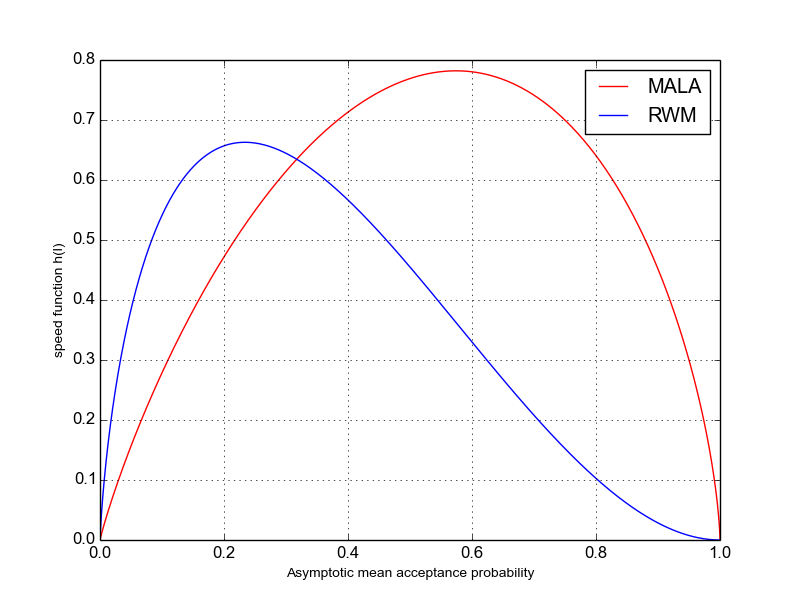
\includegraphics[width=0.75\textwidth]{speedmeasures}
 \end{center}
  \caption{Optimal acceptance probability for RWM=0.234 and MALA=0.574.}
  \label{fig:optimal acceptance probability}
\end{figure}

Through the convergence to an Gaussian random variable in Equation~(\ref{DLR-asymptotic mean acceptance probability}), the asymptotic mean acceptance probability~$\alpha^{\cdot}(l)$ can be explicitely computed and represented with the help of the culmulative density function~$\Phi$ of the standard normal distribution~\autocite[Lemma B2]{Beskos2009-2}. This convergence is also a crucial observation for later estimates. Generally speaking, the speed function varies the time-scale of the original diffusion given in Equation~(\ref{DLR-limit diffusion candidate}) by a factor~$h^{\cdot}(l)$ such that the effective time-step is reduced to $h^{\cdot}(l)\,t$ instead of $t$ as $ 0 \leq h^{\cdot}(l) \leq 1$. This results suggests choosing the value of~$l$ that maximizes the speed function~$h^{\cdot}(\cdot)$ since the limit diffusion~$z(t)$ will then explore the invariant measure as fast as possible. Obviously, the RWM and MALA algorithm have two different speed functions as the Gaussian random variables in Equation~(\ref{DLR-Gaussian RWM short}) and~(\ref{DLR-Gaussian MALA short}) differ. For practitioners, who often tune algorithms according to the acceptance probability of the simulation, it is relevant to express the maximization principle in terms of the asymptotic mean acceptance probability~$\alpha^{\cdot}(l)$. Figure~\ref{fig:optimal acceptance probability} shows that the speed function of the limit diffusion~$z(t)$ is maximized for an optimal asymptotic acceptance probability of $\alpha^{RWM}=0.234$ and $\alpha^{MALA}=0.574$, up to three decimal places. This fact is not surprising, because - as repeatedly stated - the MALA  algorithm uses gradient information on the target measure. Note that this result extends the rules for an optimal tuning of Metropolis-Hastings methods from product target measures as seen in~\autocite{Bedard2007, Roberts1997, Roberts1998} to this class of non-product measures. For further details on this type of argument for RWM and MALA, we refer to the original papers~\autocite[Section 2.3, Section 2.6]{Mattingly2010, Pillai2012}, where the idea of this presentation is taken from.

Beside this convenient rule of thumb for the optimal tuning of the two MH methods, Theorem~\ref{DLR-THM main theorem} demonstrates that, in stationarity, the computional complexity to explore the invariant measure~$\pi$ scales as~$\mathcal{O}(N^{\gamma})$, where $\gamma=1$ for the RWM and $\gamma=1/3$ for the MALA, respectively. Indeed, we accelerated the interpolant~$z^N(t)$ in Equation~(\ref{DLR-linear continuous interpolant short}) by a factor~$(\Delta t)^{-1} = N^{\gamma}$ in order to observe a diffusion limit. This shows that $\mathcal{O}(N^{\gamma})$ steps of the Markov chain~$x^N$ as defined in Equation~(\ref{DLR-MH chain from algorithm - general form}) are required for $z^N(t)$ to approximate the diffusion process $z(t)$ on a time interval~$[0,T]$. This shows impressively the idea of the diffusion limit approach to measure the computational complexity of Metropolis-Hastings methods. As the argumentation is in some sense reversely, we will recall it. Since we know that the diffusion~$z(t)$ explores its invariant measure~$\pi$, and we have to accelerate the interpolant~$z^N(t)$ of the Markov chain~$x^N$ by a factor~$N^{\gamma}$ such that $z^N(t)$ converges to $z(t)$, hence $\mathcal{O}(N^{\gamma})$ steps of the chain~$x^N$ are required to explore the measure~$\pi$.


\section{Proof of Main Theorem}
\label{sec:DLR-Proof}

In order to prove Theorem~\ref{DLR-THM main theorem} we outline the proof strategy in Section~\ref{sec:sub:DLR-Proof strategy} and introduce the discrete drift-martingale decomposition of the Metropolis-Hastings~(MH) Markov chain. This decomposition is used to show (weak) convergence of the interpolant towards the drift and the noise term of the diffusion process given in Theorem~\ref{DLR-THM main theorem} by Equation~(\ref{DLR-Thm diffusion process}). Section~\ref{sec:sub:DLR-General diffusion approximation} states and proves a general diffusion approximation for Markov chains which satisfy an appropriate drift-martingale decomposition. In Section~\ref{sec:DLR-Proof}, we finally prove Theorem~\ref{DLR-THM main theorem} by pointing to key estimates in Section~\ref{sec:DLR-Estimates}, which will show that the decomposition of the MH chain given by Equation~(\ref{DLR-MH chain from algorithm - general form}) is appropriate. The structure and main idea as well as the estimates concerning the MALA algorithm is taken from~\autocite{Pillai2012} whereas for the RWM algorithm we refer to~\autocite{Mattingly2010}. Our main contribution beside several annotations to enhance the understanding of the proof idea is the adoption of the arguments used for the MALA algorithm to the RWM case in a consitent way.

\subsection{Proof Strategy}
\label{sec:sub:DLR-Proof strategy}


The main idea for the proof of Theorem~\ref{DLR-THM main theorem} is taken from numerical analysis. In fact, we will show that the Metropolis-Hastings Markov chain~$x^N$ generated by the RWM or MALA algorithm resembles a traditional Euler-Maruyama approximation scheme~\autocite{Kloeden1992} of the diffusion~$z(t)$ given by
 \begin{equation}
 \label{DLR-Proof: Definiton: diffusion process}
  dz = -h^{\cdot}(l) (z + \mathcal{C}_s \nabla \Psi(z)) dt + \sqrt{2 h^{\cdot}(l)} d\mathcal{W}(t),
 \end{equation}
where $h^{\cdot}(l) > 0$ and $\mathcal{W}(t)$ is a $\mathcal{C}_s$-Wiener process on $\mathcal{H}^s$. This is the diffusion limit in Theorem~\ref{DLR-THM main theorem}. To illustrate the idea of the proof of the theorem, we will give a short heuristical digression on approximations schemes for stochastic differential equations~(SDEs). The Euler-Maruyama scheme for the SDE in Equation~(\ref{DLR-Proof: Definiton: diffusion process}) has the form for $0 \leq k \leq n-1$
\begin{equation}
\label{DLR-Proof: Definition Euler-Maruyama scheme of limit SDE}
\begin{split}
  Y_{k+1} & := Y_k - h^{\cdot}(l) (Y_k + \mathcal{C}_s \nabla \Psi(Y_k)) (t_{k+1} - t_k) + \sqrt{2 h^{\cdot}(l)} (\mathcal{W}(t_{k+1}) - \mathcal{W}({t_k})) \\
  & \; = Y_k + h^{\cdot}(l) \mu(Y_k) \Delta t + \sqrt{2 h^{\cdot}(l) \Delta t} \; Z_k,
\end{split}
\end{equation}
with initial condition~$Y_0 := x^{0,N}$ and the drift~$\mu: \mathcal{H}^s \to \mathcal{H}^s$ as defined in Equation~(\ref{DLR-Setting: Definition drift mu}) for an equidistant partition~$t_0 =0 < t_1 < \dots < t_{n-1} < t_n = T $ of~$[0,T]$ with $\Delta t := t_{k+1} - t_k$ and $Z_k \stackrel{D}{\sim} \mathcal{N}(0, \mathcal{C}_s)$. In the second identity, we used the fact, that $\mathcal{W}(t)$ is a $\mathcal{C}_s$-Wiener process, hence the increments are independently Gaussian distributed. Note that one may see $\mathcal{W}(t)$ equivalently as a Brownian motion on $\mathcal{H}^s$ with covariance operator~$\mathcal{C}_s$. These two notations describe the same object. Taking now the same interpolant as for the MH Markov chain as described in Equation~(\ref{DLR-linear continuous interpolant short}), we get the following rekursive expression for the Euler-Maruyama discretization~$Y(t)$ of the diffusion~$z(t)$ in the interval~$[0,T]$ for $t \in [k \Delta t, (k+1) \Delta t)$
\begin{align}
    Y(t) & \; = Y_k + \frac{t - k \Delta t}{\Delta t} (Y_{k+1} - Y_k) \nonumber  \\
    & \; = Y_k + \frac{t - k \Delta t}{\Delta t} (h^{\cdot}(l) \Delta t \, \mu(Y_k) +\sqrt{2h^{\cdot}(l) \Delta t } \; Z_k ) \nonumber \\
    & \quad \vdots \nonumber \\
    & \; = Y_0 + h^{\cdot}(l) \left[ \Delta t \sum_{i=0}^{k-1} \mu(Y_i) + (t - \Delta t) \mu(Y_k) \right] \label{DLR-Proof: Integralapproximation mu} \\ 
    & \qquad + \sqrt{2 h^{\cdot}(l)} \left\{ \sqrt{ \Delta t} \sum_{i=0}^{k-1} Z_i +  \frac{t - \Delta t}{\sqrt{\Delta t}} Z_k \right\} \label{DLR-Proof: Wiener process approximation}
\end{align}
Following the methodology of stochastic approximations schemes, we have to prove convergence of the quantity in the angular brackets in Equation~(\ref{DLR-Proof: Integralapproximation mu}) to the drift integral~$\int_0^t \mu (t) dt$ of the original SDE and we have to show an \textit{invariance principle}, in the sense of a generalization of Donsker's Theorem as in~\autocite{Revuz2005}, for the quantity in the curly brackets in Equation~(\ref{DLR-Proof: Wiener process approximation}). Such an invariance principle states  that a rescaled sum of random variables, as the quantity in the curly brackets, converges weakly to a Wiener process~$\mathcal{W}(t)$ on $\mathcal{H}^s$ with a covariance operator~$\mathcal{C}_s$. 



Keeping this in mind, let $\mathcal{F}_k$ denote the sigma algebra generated by~$\{ x^{i,N}, \xi^{i,N}, \gamma^{i,N} : i \leq k  \}$. We denote the conditional expectation by~$\mathbb{E}[|\mathcal{F}_k]$. We define now the \textit{drift-martingale decomposition} of the Metropolis-Hastings chain~$x^N = \{ x^{k,N} \}_{k \geq 0}$ by introducing the drift function~$d^N: \mathcal{H}^s \to \mathcal{H}^s$ given by
\begin{equation}
\label{DLR-Proof: Definition drift function d^N}
d^N (x) := \left(  h^{\cdot}(l) \Delta t \right)^{-1} \mathbb{E} \left[ x^{1,N} - x^{0,N} | x^{0,N} = x \right] 
\end{equation}
and the martingale difference array~$\{ \Gamma^{k,N} (x^{k,N}, \xi^{k,N})= \Gamma^{k,N} : k \geq 0 \}$ defined by
\begin{equation}
 \label{DLR-Proof: Definiton martingale difference array}
 \Gamma^{k,N} := \left( 2 h^{\cdot}(l) \Delta t \right)^{-1/2} \left( x^{k+1,N} -x^{k,N} - h^{\cdot}(l) \Delta t d^N (x^{k,N})  \right).
\end{equation}
For the drift-martingale decomposition the natural time step is given by $\Delta t := N^{-\gamma}$ as in Theorem~\ref{DLR-THM main theorem}. By definition, $\Gamma^{k,N}$ is a $\mathcal{F}_k$-martingale for any~$N\geq1$. The drift-martingale decomposition of the Markov chain~$\{ x^{k,N} \}_{k}$ then reads
\begin{equation}
 \label{DLR-Proof: Definition drift-martingale decomposition}
 x^{k+1,N} - x^{k,N} = h^{\cdot}(l) \Delta t \, d^N(x^{k,N}) + \sqrt{2 h^{\cdot}(l) \Delta t} \, \Gamma^{k,N}.
\end{equation}
This identitiy follows directly by inserting the definition of the drift martingale array. According to the methodology of numerical analysis, we now interpolate our time-discrete chain continuously and piecewise linearly as defined in Equation~(\ref{DLR-linear continuous interpolant short}) and used in the heuristic digression. Thus the interpolant~$z^N(t)$, $t \in [0,T]$, has the form 
\begin{align}
  z^N(t) & \; = x^{0,N} + h^{\cdot}(l) \left[ \Delta t \sum_{i=0}^{k-1} d^N(x^{i,N}) + (t - \Delta t) d^N(x^{k,N}) \right] \label{DLR-Proof: Integralapproximation d^N} \\ 
  & \qquad + \sqrt{2 h^{\cdot}(l)} \left\{ \sqrt{ \Delta t} \sum_{i=0}^{k-1} \Gamma^{i,N} +  \frac{t - \Delta t}{\sqrt{\Delta t}} \Gamma^{k,N} \right\} \label{DLR-Proof: Gamma approximation}
\end{align}
for $k \Delta t \leq t  < (k+1) \Delta t $ and $\Delta t = N^{-\gamma}$. In order to show now weak convergence in $C([0,T];\mathcal{H}^s)$ of the interpolant~$z^N(t)$ to the diffusion~$z(t)$ given in Equation~(\ref{DLR-Proof: Definiton: diffusion process}), one has to verify that the quantity in the angular brackets in Equation~(\ref{DLR-Proof: Integralapproximation d^N}) converges to the drift of $z(t)$ and the quantity in the curly brackets in Equation~(\ref{DLR-Proof: Gamma approximation}) converges to a $\mathcal{C}_s$-Wiener process in $\mathcal{H}^s$, i.e.,
\begin{equation}
  \label{DLR-Proof: Definition W^N}
  \begin{split}
   \Delta t \sum_{i=0}^{k-1} d^N(x^{i,N}) + (t - \Delta t) d^N(x^{k,N}) \Longrightarrow \int_0^t \mu(z(t)) dt, \\
   W^N(t) := \sqrt{ \Delta t} \sum_{i=0}^{k-1} \Gamma^{i,N} +  \frac{t - \Delta t}{\sqrt{\Delta t}} \Gamma^{k,N} \Longrightarrow \mathcal{W}(t), \\
 \end{split}
\end{equation}
where $\Longrightarrow$ denotes weak convergence in $C([0,T];\mathcal{H}^s)$ for $N \to \infty$ and $\mathcal{W}(t)$ denotes a Wiener process on $\mathcal{H}^s$ with  covariance operator~$\mathcal{C}_s$. A key point for the convergence of the drift term is the fact that quantity~$Q^N_{\cdot}(x, \xi^N)$ has a Gaussian behavior for large~$N$ such that one can give a quantitative version of the approximation~$ d^N(x) \approx \mu(x) $, see Lemma~\ref{DLR: Lemma Dirft approximation}. To prove the convergence of the \textit{noise}~$W^N(t) \in C([0,T];\mathcal{H}^s)$, we establish an invariance principle for the rescaled version of the martingale difference array given by $W^N(t)$. Indeed, Proposition~\ref{Invariance principle} proves the stronger result
\begin{equation*}
  (x^{0,N}, W^N) \Longrightarrow (z^0, \mathcal{W}),
\end{equation*}
where $\Longrightarrow$ denotes weak convergence in $\mathcal{H}^s \times C([0,T];\mathcal{H}^s)$, and $z^0 \stackrel{D}{\sim} \pi$ is independent of the limiting Wiener process~$\mathcal{W}(t)$. Using this invariance principle for~$W^N$ and the fact of additive noise in the diffusion limit~$z(t)$, we deduce the weak convergence of~$z^N$ to $z$ in $ C([0,T];\mathcal{H}^s)$ from a continuous  mapping argument (It\={o} map). This continuous mapping argument, which we will now outline, allows us to manage the transfer from the drift term with $d^N(x)$ given in Equation~(\ref{DLR-Proof: Integralapproximation d^N}) to the desired drift~$ \int_0^t \mu(z) du$ of the limiting SPDE given in Equation~(\ref{DLR-Proof: Definiton: diffusion process}). For a rigorous proof, we refer to Proposition~\ref{DLR-Proof: Proposition General diffusion approximation}.

Define the It\={o} map~$\Theta$ for any $\omega \in C([0,T];\mathcal{H}^s)$ by 
\begin{equation*}
 \Theta : \mathcal{H}^s \times C([0,T];\mathcal{H}^s) \to C([0,T];\mathcal{H}^s)
\end{equation*}
which maps~$(z^0, \omega)$ to the unique solution of the integral equation
\begin{equation}
  z(t) := z^0 - h^{\cdot}(l) \int_0^t \mu(z) du + \sqrt{2 h^{\cdot}(l)} \omega(t) \qquad \forall t \in [0,T].
\end{equation}
Note that $z := \Theta (z^0, \mathcal{W})$ solves the limiting SPDE given in Theorem~\ref{DLR-THM main theorem}:
\begin{equation}
 z(t) = z^0 -  h^{\cdot}(l) \int_0^t (z(u) + \mathcal{C}_s \nabla \Psi(z(u))) du + \sqrt{2 h^{\cdot}(l)} \mathcal{W}(t) \qquad \forall t \in [0,T],
\end{equation}
where~$\mathcal{W}(t)$ is a $ \mathcal{H}^s $-valued  $ \mathcal{C}_s $-Wiener process. To represent the interpolant~$z^N(t)$ given in Equations~(\ref{DLR-Proof: Integralapproximation d^N}) and~(\ref{DLR-Proof: Gamma approximation}) as an integral equation, we introduce the piecewise constant interpolant~$\bar{z}(t)$ of the chain~$x^N$ which is defined by
\begin{equation}
  \label{DLR: Proof Strategy Definition piecewise constant interpolant}
  \bar{z}(t) := x^{k,N} \quad \text{ for } k \Delta t \leq t < (k+1) \Delta t.
\end{equation}
Using this definition it follows that the continuous piecewise linear interpolant~$z^N(t)$ satisfies
\begin{equation}
  z^N(t) = x^{0,N} +  h^{\cdot}(l) \int_0^t d^N(\bar{z}(u)) du + \sqrt{2 h^{\cdot}(l)} W^N(t) \qquad \forall t \in [0,T].
\end{equation}
Exploiting the closeness of $d^N(\cdot)$ and $\mu(\cdot)$, and of $\bar{z}(t)$ and $z^N(t)$, we will see that there exists a continuous process~$\widehat{W}^N \Longrightarrow \mathcal{W}$ as $N$ goes to infinity such that
\begin{equation*}
 z^N(t) = x^{0,N} +  h^{\cdot}(l) \int_0^t \mu(z^N(u)) du + \sqrt{2 h^{\cdot}(l)} \widehat{W}^N(t) \qquad \forall t \in [0,T].
\end{equation*}
Therefore, we may write $z^N = \Theta (x^{0,N}, \widehat{W}^N)$. Finally, by the continuity of the It\={o} map~$\Theta$, we conclude from the continuous mapping theorem that
\begin{equation*}
  z^N = \Theta (x^{0,N}, \widehat{W}^N) \Longrightarrow \Theta (z^0, \mathcal{W}) = z \qquad \text{  as } N \to \infty.
\end{equation*}
This will finish the proof of Theorem~\ref{DLR-THM main theorem} since a suitable scaled version of the Metropolis-Hastings Markov chain generated by the RWM or MALA algorithm converges weakly to the expected limit Langevin diffusion process.



\subsection{General Diffusion Approximation}
\label{sec:sub:DLR-General diffusion approximation}

This section is devoted to a general diffusion approximation result containing the contiunous mapping argument as described in Section~\ref{sec:sub:DLR-Proof strategy} and is taken from~\autocite[Section 3.2]{Pillai2012}. We impose three requirements on a general drift-martingale decompostion of a Markov chain such that this decomposition which resembles a traditional Euler-Maruyama scheme converges weakly to a suitable limit SDE. This result is the heart of the matter of the proof of Theorem~\ref{DLR-THM main theorem}. In Section~\ref{sec:sub:DLR-Proof} we will varify that the drift-martingale decomposition of the Metropolis-Hastings Markov chain obtained by the RWM or MALA algorithm in the Hilbert space setting fulfills these imposed conditions which  will finally finish the proof of Theorem~\ref{DLR-THM main theorem}.

In this section we step back and consider a general sequence of Markov chains~$x^N = \{ x^{k,N} \}_{k\geq0}$ evolving at stationarity in a separable Hilbert space~$\mathcal{H}^s$. We define the drift function~$d^N: \mathcal{H}^s \to \mathcal{H}^s$ as in Equation~(\ref{DLR-Proof: Definition drift function d^N}) as well as the martingale difference array~$\{\Gamma^{k,N}\}_{k\geq0}$ defined in Equation~(\ref{DLR-Proof: Definiton martingale difference array}) and introduce the drift-martingale decomposition
\begin{equation}
  \label{DLR-Proof: drift-martingale decomposition for general diffusion approximation}
 x^{k+1,N} - x^{k,N} = h^{\cdot}(l) \Delta t \, d^N(x^{k,N}) + \sqrt{2 h^{\cdot}(l) \Delta t} \, \Gamma^{k,N},
\end{equation}
with $h^{\cdot}(l)>0$ and $\Delta t$ a time-step decreasing to zero for $N$ going to infinity. Moreover, we define a rescaled and interpolated version of the martingale difference array denoted by~$W^N \in C([0,T];\mathcal{H}^s)$ given in Equation~(\ref{DLR-Proof: Definition W^N}).


\begin{proposition}\autocite[Proposition 3.1]{Pillai2012}(General diffusion approximation for Markov chains)
  \label{DLR-Proof: Proposition General diffusion approximation}
  Consider a separable Hilbert space~$(\mathcal{H}^s, \langle \cdot, \cdot \rangle_s$ and a sequence of~$\mathcal{H}^s$-valued Markov chains~$x^N = \{ x^{k,N} \}_{k \geq 0}$ with invariant distribution~$\pi^N$. Suppose that the Markov chains start at stationarity~$x^{0,N} \stackrel{D}{\sim} \pi^N$ and the drift-martingale decomposition given in Equation~(\ref{DLR-Proof: drift-martingale decomposition for general diffusion approximation}) satisfies the following assumptions:
  \begin{enumerate}
    \item[(1)] Convergence of initial conditions: $\pi^N$ converges in distribution to the probability measure~$\pi$ where $\pi$ has a finite moment, that is, $\mathbb{E}^{\pi}[\|x\|_s]<\infty$. 
    \item[(2)] Convergence of the drift: there exists a globally Lipschitz function~$\mu:\mathcal{H}^s \to \mathcal{H}^s$ that satisfies
    \begin{equation*}
      \lim_{N \to \infty} \mathbb{E}^{\pi^N}[ \|  d^N(x) - \mu(x) \|_{s} ] = 0 \qquad \text{ for all } x \in \mathcal{H}^s.
    \end{equation*}
    \item[(3)] Invariance principle: the sequence~$(x^{0,N}, W^N)$, defined by Equation~(\ref{DLR-Proof: Definition W^N}) converges weakly in $\mathcal{H}^s \times C([0,T]; \mathcal{H}^s)$ to~$(z^0, \mathcal{W})$ where~$z^0 \stackrel{D}{\sim} \pi$, and $\mathcal{W}$ is a $\mathcal{H}^s$-valued $\mathcal{C}_s$-Wiener process, independent from~$z^0$.
  \end{enumerate}
  
  Then the sequence of rescaled interpolants~$z^N \in C([0,T]; \mathcal{H}^s)$, defined by Equation~(\ref{DLR-linear continuous interpolant short}), converges weakly in $ C([0,T]; \mathcal{H}^s)$ to $z \in  C([0,T]; \mathcal{H}^s)$ given by
  \begin{equation*}
    \begin{split}
     dz(t) & \;=   h^{\cdot}(l) \mu(z(t)) dt + \sqrt{2 h^{\cdot}(l)} d\mathcal{W}(t) \qquad \forall t \in [0,T], \\
     z(0) & \; \stackrel{D}{\sim} \pi.\\
    \end{split}
  \end{equation*}
  Here $\mathcal{W}(t)$ is a Wiener process in~$\mathcal{H}^s$ with covariance operator~$\mathcal{C}_s$ and initial condition~$z^0 \stackrel{D}{\sim} \pi$ independent of $\mathcal{W}$.

\end{proposition}

\begin{proof}
  The structure of the proof is taken from~\autocite[Proposition 3.1]{Pillai2012}.  Recall the basic idea of comparing the Metropolis-Hastings Markov chain~$\{ x^{k,N} \}_{k \geq 1}$ to an Euler-Maruyama approximation scheme of the limit diffusion process~$z(t)$ given in Equation~(\ref{DLR-Proof: Definiton: diffusion process}). We start with tracking  the error in this Euler-Maruyama approximation argument. Let the chain start in stationarity, i.e.\,$x^{0,N} \stackrel{D}{\sim} \pi^N$. Define the piecewise constant interpolant~$\bar{z}(t)$ as in Equation~(\ref{DLR: Proof Strategy Definition piecewise constant interpolant}). Inserting~$\bar{z}^N(t)$ in the representation of the piecewise linear interpolant~$z(t)$ of the chain~$\{ x^{k,N} \}_{k \geq 1}$ given in Equations~(\ref{DLR-Proof: Integralapproximation d^N}) and~(\ref{DLR-Proof: Gamma approximation}) allows us to deduce that
  \begin{equation}
    \label{DLR: Proposition General diffusion approximation interpolant representation}
    \begin{split}
      z^N(t) & = x^{0,N} + h^{\cdot}(l) \int_0^t d^N(\bar{z}^N(u)) du + \sqrt{2 h^{\cdot}(l)} \; W^N(t) \\
      & = z^{0,N} + h^{\cdot}(l) \int_0^t \mu(z^N(u)) du + \sqrt{2 h^{\cdot}(l)} \;\widehat{W}^N(t),
    \end{split}
  \end{equation} 
  where the continuous noise process~$W^N(t) \in C([0,T]; \mathcal{H}^s)$ is defined by Equation~(\ref{DLR-Proof: Definition W^N}) and the corrected noise process~$\widehat{W}^N(t)\in C([0,T]; \mathcal{H}^s) $ is given by
  \begin{equation}
    \widehat{W}^N(t) :=  W^N(t) + \sqrt{\frac{h^{\cdot}(l)}{2}} \int_0^t [d^N(\bar{z}^N(u)) - \mu(z^N(u))] du.
  \end{equation}
  Hence, $\widehat{W}^N(t)$ incorporates the error due to the change from~$d^N(\bar{z}^N(u))$ to $\mu(z^N(u))$; the change of the interpolant and the drift function. By assumption, we know that the uncorrected noise process~$W^N(t)$ fulfills an invariance principle to deduce that also the corrected noise process~$\widehat{W}^N(t)$ converges to a $\mathcal{C}_s$-Wiener process on~$\mathcal{H}^s$ and that $z^N(t)$ given in Equation~(\ref{DLR: Proposition General diffusion approximation interpolant representation}) converges to the diffusion given in Equation~(\ref{DLR-Thm diffusion process}), we exploit a continuous mapping argument. Define the It\={o} map~$\Theta : \mathcal{H}^s \times C([0,T]; \mathcal{H}^s) \to  C([0,T]; \mathcal{H}^s)$ that maps~$(z_0, \omega) $ to the unique solution~$z \in  C([0,T]; \mathcal{H}^s)$ of the integral equation
  \begin{equation}
    \label{DLR: Proposition General Diffusion approximation integral equation}
   z(t) := z^0 + h^{\cdot}(l) \int_0^t \mu(z) du + \sqrt{2 h^{\cdot}(l)} \omega(t) \qquad \forall t \in [0,T].
  \end{equation}
  Therefore, the representation of~$z^N(t)$ given in Equation~(\ref{DLR: Proposition General diffusion approximation interpolant representation}) is equivalent to~$z^N = \Theta (x^{0,N}, \widehat{W}^N )$. To apply the continuous mapping argument and conclude that~$z^N $ converges weakly to~$ z(t)$ in~$ C([0,T]; \mathcal{H}^s)$ we have to prove first that the error in the correction term of~$\widehat{W}^N(t)$ has no effect on the asymptotic behavior, in the sense that we can also establish an invariance principle for~$\widehat{W}^N(t)$ in a second step we have to prove that the It\={o} map~$\Theta : \mathcal{H}^s \times C([0,T]; \mathcal{H}^s) \to  C([0,T]; \mathcal{H}^s)$ is well-defined in the sense that it is continuous and that the integral equation given in Equation~(\ref{DLR: Proposition General Diffusion approximation integral equation}) has a unique (strong) and continuous solution.
  
  \begin{claim}
   \label{DLR: Proposition General diffusion approximation: Claim 1: convergence of corrected noise}
   The pair~$(x^{0,N}, \widehat{W}^N)$ converges weakly to~$(z^0, \mathcal{W})$ in $\mathcal{H}^s \times C([0,T]; \mathcal{H}^s)$, where $\mathcal{W}$ is a $\mathcal{H}^s$-valued $\mathcal{C}_s$-Wiener process, independent from~$z^0$ as given in Proposition~\ref{DLR-Proof: Proposition General diffusion approximation}.
  \end{claim}
  \begin{proof}(of Claim~\ref{DLR: Proposition General diffusion approximation: Claim 1: convergence of corrected noise})~\autocite[Proposition 3.1]{Pillai2012}
    
    It is assumed that~$(x^{0,N}, W^N)$ converges weakly to~$(z^0, \mathcal{W})$ in $\mathcal{H}^s \times C([0,T]; \mathcal{H}^s)$ and $\mathcal{W}$ is independent from~$z^0$. Hence it suffices to prove that~$\widehat{W}^N$ converges weakly to~$W^N$ in~$C([0,T]; \mathcal{H}^s)$. To prove this, note that, in a separable Hilbert space, if the sequence~$\{ a_n \}_{n \in \mathbb{N}}$ converges weakly to~$a$, and the sequence~$\{ b_n \}_{n \in \mathbb{N}}$ converges in probability to zero, then the sequence~$\{ a_n + b_n \}_{n \in \mathbb{N}}$ converges weakly to~$a$. That result is also known as Slutky's theorem. Due to this fact, it is enough to verify that
    \begin{equation}
      \lim_{N\to \infty} \mathbb{E}^{\pi^N} \left[ \int_0^T  \| d^N(\bar{z}^N(u)) - \mu(z^N(u)) \|_s du \right] = 0.
    \end{equation}
    For any time~$ k \Delta t \leq u < (k+1)\Delta t $, the definition of~$\bar{z}^N(t)$ and the stationarity conserving of the chain shows that
    \begin{align*}
      \| d^N(\bar{z}^N(u)) - \mu(\bar{z}^N(u)) \|_s & = \| d^N(x^{k,N})) - \mu(x^{k,N}) \|_s \\
      & \stackrel{D}{\sim} \| d^N(x^{0,N})) - \mu(x^{0,N}) \|_s, \\
      \| \mu(\bar{z}^N(u)) - \mu(z^N(u)) \|_s & = \|  \mu \|_{Lip} \cdot \| x^{k+1,N} - x^{k,N} \|_s \\
      & \stackrel{D}{\sim} \|  \mu \|_{Lip} \cdot \| x^{1,N} - x^{0,N} \|_s,
    \end{align*}
    where in the last step we hae used the Lipschitz continuity of the drift~$\mu: \mathcal{H}^s \to \mathcal{H}^s$ as proven in Corollary~\ref{DLR-Setting: Corollary: drifts are Lipschitz} and the fact that~$\| \bar{z}^N(u) - z^N(u) \|_s \leq \| x^{k+1,N} - x^{k,N} \|_s$.  Consequently, by using the triangle inequality
    \begin{align*}
     \mathbb{E}^{\pi^N} \left[ \int_0^T  \| d^N(\bar{z}^N(u)) - \mu(z^N(u)) \|_s du \right] & \leq T \cdot \mathbb{E}^{\pi^N} \left[ \| d^N(x^{0,N})) - \mu(x^{0,N}) \|_s \right] \\
     & \qquad + T \cdot  \|  \mu \|_{Lip} \cdot  \mathbb{E}^{\pi^N} \left[ \| x^{1,N} - x^{0,N} \|_s \right] .
    \end{align*}
    The first term goes to zero by assumption (Convergence of the drift) and the second term also converges to zero as we postpone to Lemma~\ref{DLR: Lemma jump size of order(sqrt(Delta t))} that the jump size~$\mathbb{E}^{\pi^N} \left[ \| x^{1,N} - x^{0,N} \|_s \right]$ is of order~$\mathcal{O}(\sqrt{\Delta t})$ and thus converges to zero. Therefore, we conclude that~$\widehat{W}^N$ converges weakly to~$W^N$ in~$C([0,T]; \mathcal{H}^s)$ and this finishes the proof of Claim~\ref{DLR: Proposition General diffusion approximation: Claim 1: convergence of corrected noise}.
  \end{proof}   
  
  \begin{claim}
    \label{DLR: Proposition General diffusion approximation: Claim 2: Ito map}
  Fix~$T>0$. Let~$z^0 \in \mathcal{H}^s$ and $\omega \in C([0,T];\mathcal{H}^s)$. Then the integral equation of the It\={o} map~$\Theta : \mathcal{H}^s \times C([0,T]; \mathcal{H}^s) \to  C([0,T]; \mathcal{H}^s)$ defined by Equation~(\ref{DLR: Proposition General Diffusion approximation integral equation}) has an unique solution~$z \in C([0,T];\mathcal{H}^s)$. Furthermore, the It\={o} map~$\Theta$ is continuous.
  \end{claim}
  
  \begin{proof} (of Claim~\ref{DLR: Proposition General diffusion approximation: Claim 2: Ito map})~\autocite[Lemma 3.7]{Mattingly2010}
    The proof is based on the contraction mapping theorem which shows existence and uniqueness for ordinary differential equations with Lipschitz coefficients and Gronwall's inequality which is used to show continuity of the It\={o} map~$\Theta$. For the existence and uniqueness of the SDE given by Equation~(\ref{DLR: Proposition General Diffusion approximation integral equation}) define the approximating sequence~$\{ z^{(n)}(t) \}_{n \in \mathbb{N}} $ given by
    \begin{equation}
      \begin{split}
       z^{(n+1)}(t) & := z^0 + h^{\cdot}(l) \int_0^t \mu (z^{(n)}(u)) du + \sqrt{2 h^{\cdot}(l)} \omega(t) \\
       z^{(0)}(t) & := z^0
      \end{split}
    \end{equation}
    for an arbitrary~$z^0 \in \mathcal{H}^s$ and $\omega \in C([0,T];\mathcal{H}^s)$. This sequence is also known as Picard-Lindel\"{o}ff iteration. Since the Lipschitz continuity of~$\mu: \mathcal{H}^s \to \mathcal{H}^s$, it is readily shown that the map~$F: C([0,T];\mathcal{H}^s) \to C([0,T];\mathcal{H}^s)$ defined by~$z(t) \mapsto z^0 + h^{\cdot}(l) \int_0^t \mu (z(u)) du + \sqrt{2 h^{\cdot}(l)} \omega(t)$ is a contraction. Indeed, for~$z_1(\cdot), z_2(\cdot) \in C([0,T];\mathcal{H}^s)$, we obtain that
    \begin{align*}
      \sup_{t \in [0,T]} \| F(z_1(t)) - F(z_2(t)) \|_{s} & \leq \sup_{t \in [0,T]} \int_0^t \| \mu(z_1(u)) - \mu(z_2(u)) \|_{s} du \\
      & \leq \int_0^T \sup_{t \in [0,T]} \| \mu(z_1(t)) - \mu(z_2(t)) \|_{s} du \\
      & \leq \| \mu \|_{Lip} \cdot T \cdot \sup_{t \in [0,T]} \| z_1(t) - z_2(t) \|_{s},
    \end{align*}
    where~$C([0,T];\mathcal{H}^s)$ is a Banach space with the supremum norm~$\sup_{t \in [0,T]} \| f(t) \|_s $ for $f \in C([0,T];\mathcal{H}^s)$. For sufficently small~$T>0$, the constant~$\vartheta := \| \mu \|_{Lip} \cdot T$ is smaller than one and in particular~$\vartheta $ is independent from the initial value~$z^0 \in \mathcal{H}^s$. Hence a Banach fix point argument shows that the mapping~$F$ has an unique fix point in~$C([0,T];\mathcal{H}^s)$. By construction, this fix point is a solution for the integral equation given in Equation~(\ref{DLR: Proposition General Diffusion approximation integral equation}) and it is unique by the fix point theorem. Repeated application of the same idea extends this existence and uniqueness result to arbitrary time-intervalls. 
    
    To prove continuity of the It\={o} map~$\Theta : \mathcal{H}^s \times C([0,T]; \mathcal{H}^s) \to  C([0,T]; \mathcal{H}^s)$, let~$z_i (\cdot)$ solve integral equation defined in Equation~(\ref{DLR: Proposition General Diffusion approximation integral equation}) with~$(z^0, \omega) = (z^0_i, \omega_i), i = 1,2$. Subtracting both equations and using again the global Lipschitz continuity of~$\mu$ on~$\mathcal{H}^s$, we have
    \begin{equation*}
     \| z_1(t) - z_2(t) \|_s  \leq  \| z_1^0 - z_2^0 \|_s + \| \mu \|_{Lip} \cdot \int_0^t  \| z_1(u) - z_2(u) \|_s du + \sqrt{2 h^{\cdot}(l)}  \| \omega_1(t) - \omega_2(t) \|_s.
    \end{equation*}
    Hence, we conclude that
    \begin{align*}
      \sup_{0 \leq t \leq T} \| z_1(t) - z_2(t) \|_s &  \leq  \| z_1^0 - z_2^0 \|_s + \| \mu \|_{Lip} \cdot \int_0^T \sup_{0 \leq \tau \leq u}  \| z_1(\tau) - z_2(\tau) \|_s du \\
      & \quad + \sqrt{2 h^{\cdot}(l)} \sup_{0 \leq t \leq T}  \| \omega_1(t) - \omega_2(t) \|_s.
    \end{align*}
    To apply Gronwall's inequality, we define the constant $\beta := \| \mu \|_{Lip} $, the continuous function~$g : [0,T] \to \mathbb{R}$ by
    \begin{equation*}
     g (t) := \sup_{0 \leq \tau \leq t} \| z_1(\tau) - z_2(\tau) \|_s,
    \end{equation*}
    furthermore let~$\alpha: [0,T] \to \mathbb{R}$ be given by
    \begin{equation*}
     \alpha(t) := \| z_1^0 - z_2^0 \|_s + \sqrt{2 h^{\cdot}(l)} \sup_{0 \leq \tau \leq t}  \| \omega_1(\tau) - \omega_2(\tau) \|_s,
    \end{equation*}
    which is integrable as $\omega_i \in  C([0,T]; \mathcal{H}^s)$ for~$i = 1,2$. Then $ 0 \leq u(t) \leq \alpha(t) + \beta  \int_0^t u(\tau)d\tau $. Hence, by Gronwall's inequality~\autocite{Karatzas2000} for $0 \leq t \leq T$,
    \begin{align*}
      \sup_{0 \leq \tau \leq t} \| z_1(\tau) - z_2(\tau) \|_s = g(t) & \leq \alpha(t) + \beta \cdot \int_0^t \alpha(s) e^{\beta (t-u)}du  \\
      & \leq (1+ \beta e^{\beta t}) \alpha(t)\\
      & \leq (1+ \| \mu \|_{Lip} e^{\| \mu \|_{Lip} \cdot t}) \| z_1^0 - z_2^0 \|_s \\
      & \qquad + \sqrt{2 h^{\cdot}(l)} \sup_{0 \leq \tau \leq t}  \| \omega_1(\tau) - \omega_2(\tau) \|_s \\
      & = M_1 \cdot \| z_1^0 - z_2^0 \|_s + M_2 \cdot \sup_{0 \leq \tau \leq t}  \| \omega_1(\tau) - \omega_2(\tau) \|_s.
    \end{align*}
    Thus, if $(z^0_1, \omega_1) \Longrightarrow (z^0_2, \omega_2)$ in $\mathcal{H}^s \times C([0,T]; \mathcal{H}^s)$ then $\| z_1^0 - z_2^0 \|_s \to 0$ and $\sup_{0 \leq \tau \leq t}  \| \omega_1(\tau) - \omega_2(\tau) \|_s \to 0$and hence, $\sup_{0 \leq \tau \leq t} \| z_1(\tau) - z_2(\tau) \|_s \to 0$. This proves that the It\={o} map~$\Theta : \mathcal{H}^s \times C([0,T]; \mathcal{H}^s) \to  C([0,T]; \mathcal{H}^s)$ is continuous. This finishes the proof of Claim~\ref{DLR: Proposition General diffusion approximation: Claim 2: Ito map}.
     
  \end{proof}   
  
  With these two porperties, we can now conclude the result of Proposition~\ref{DLR-Proof: Proposition General diffusion approximation} by a continuous mapping argument. We have proved that~$(x^{0,N}, \widehat{W}^N)$ converges weakly to~$(z^0, \mathcal{W})$ in~$\mathcal{H}^s \times C([0,T];\mathcal{H}^s)$, and the It\={o} map~$\Theta : \mathcal{H}^s \times C([0,T]; \mathcal{H}^s) \to  C([0,T]; \mathcal{H}^s)$ is a continuous function. Thus the continuous mapping theorem~\autocite[Theorem 4.27]{Kallenberg2001} shows that
  \begin{equation*}
    z^N = \Theta (x^{0,N}, \widehat{W}^N) \Longrightarrow \Theta (z^0, \mathcal{W}) = z \qquad \text{  as } N \to \infty,
  \end{equation*}
  where $ \Longrightarrow$ denotes weak convergence in~$\mathcal{H}^s \times C([0,T]; \mathcal{H}^s)$. This completes the proof of Proposition~\ref{DLR-Proof: Proposition General diffusion approximation}.
  
   
\end{proof}


\subsection{Proof of Theorem~\ref{DLR-THM main theorem}}
\label{sec:sub:DLR-Proof}

To finish the proof of Theorem~\ref{DLR-THM main theorem} we have to check the conditions imposed on  the sequence of RWM and MALA Markov chains given in Equation~(\ref{DLR-MH chain from algorithm - general form}) in Proposition~\ref{DLR-Proof: Proposition General diffusion approximation}. Additionally, we postponed a claim concerning the expected one step mean of these chains. The key estimates are proved subsequently in Section~\ref{sec:DLR-Estimates}.

For the imposed conditions of Proposition~\ref{DLR-Proof: Proposition General diffusion approximation}, we have
 \begin{enumerate}
    \item[(1)] Convergence of initial conditions: Lemma~\ref{DLR-Proof: Lemma Convergence of pi^N to pi} proves that the sequence of probability measures~$\pi^N$ converges in distribution to the probability measure~$\pi$ where $\pi$ has a finite moment, that is, $\mathbb{E}^{\pi}[\|x\|_s]<\infty$. 
    \item[(2)] Convergence of the drift: By Corollary~\ref{DLR-Setting: Corollary: drifts are Lipschitz} the drift of the limit diffusion~$z(t)$ given in Equation~(\ref{DLR-Thm diffusion process}) is globally Lipschitz in~$\mathcal{H}^s$. Furthermore Lemma~\ref{DLR: Lemma Dirft approximation} states that 
    \begin{equation*}
      \lim_{N \to \infty} \mathbb{E}^{\pi^N}[ \|  d^N(x) - \mu(x) \|_{s} ] = 0 \qquad \text{ for all } x \in \mathcal{H}^s.
    \end{equation*}
    \item[(3)] Invariance principle: Proposition~\ref{Invariance principle} proves that the sequence~$(x^{0,N}, W^N)$, defined by Equation~(\ref{DLR-Proof: Definition W^N}) converges weakly in $\mathcal{H}^s \times C([0,T]; \mathcal{H}^s)$ to~$(z^0, \mathcal{W})$ where~$z^0 \stackrel{D}{\sim} \pi$, and $\mathcal{W}$ is a $\mathcal{H}^s$-valued $\mathcal{C}_s$-Wiener process, independent from~$z^0$.
  \end{enumerate}
Additionally, Lemma~\ref{DLR: Lemma jump size of order(sqrt(Delta t))} states that the expected one step means of the Metropolis-Hastings chains are of order~$\mathcal{O}(\sqrt{\Delta t})$. Consequently, the proof of Theorem~\ref{DLR-THM main theorem} is completed.



\section{Key Estimates}
\label{sec:DLR-Estimates}

In the previous section, we stated and proved a general diffusion approximation result for Markov chains. To link this theory to the Metropolis-Hastings Markov chain generated by the RWM and MALA algorithm in the Hilbert setting as defined in Equation~(\ref{DLR-MH chain from algorithm - general form}), we have to verify several properties of the drift-martingale decomposition of those Markov chain sequences. Beside some general and technical results like the convergence of the approximated measures~$\pi^N$ to the infinite dimensional target measure~$\pi$ in Section~\ref{sec:sub: DLR - Tehnical Lemmas}, there are three main issues to understand. First the Gaussian behavior of the quantity~$Q^{N}_{\cdot}(x, \xi^N)$ in the acceptance probability of the appropriate algorithm, see Section~\ref{sec:sub:DLR - Gaussian approximation}, which will be needed to give quantitative versions of the drift approximation (Section~\ref{sec:sub:DLR - Drift Approximation}) and finally the noise approximation (Section~\ref{sec:sub:DLR - Noise Approximation}).

The main statement, Theorem~\ref{DLR-THM main theorem}, holds for the RWM and MALA algorithm equally. Also the general proof strategy is the same. But to show the necessary properties of the drift-martingale decomposition of the Metropolis-Hastings Markov chain generated by the MH method, we have to distinguish between the two algorithms in this section. To do so we state several results divided into a RWM and MALA part seperately. As we adopt the proof method introduced in~\autocite{Pillai2012} to the RWM algorithm, we mostly refer to~\autocite{Pillai2012} for proofs concerning the MALA algorithm and we prove only the result for the RWM algorithm.



\subsection{Technical Lemmas} 
\label{sec:sub: DLR - Tehnical Lemmas}

As a first result we show the convergence of the approximations~$\pi^N$ to~$\pi$. We have seen that the sequence~$\{ \pi^N \}$ converges to~$\pi$ in the Hellinger metric. Furthermore, the normalizing constants~$M_{\Psi^N}$ are uniformly bounded and we use this fact to obtain uniform bounds on moments of functionals in~$\mathcal{H}^s$ under~$\pi^N$ and weak convergence of~$\{ \pi^N \}$ to~$\pi$.

\begin{lemma}\autocite[Lemma 3.5, Lemma 4.3]{Mattingly2010, Pillai2012}
  \label{DLR-Proof: Lemma Convergence of pi^N to pi}
  Under Assumption~\ref{DLR-Setting: Assumptions on C and Psi} the normalization constants~$M_{\Psi^N}$ are uniformly bounded, i.e., $ \sup_{N \in \mathbb{N}} M_{\Psi^N} < \infty$, so that for any $\pi_0$-measurable functional~$f: \mathcal{H}^s \to \mathbb{R}$ and any $p\geq 1$, we have
  \begin{equation*}
    \sup_{N \in \mathbb{N}} \mathbb{E}^{\pi^N} [| f(x) |^p] \lesssim \mathbb{E}^{\pi_0}[|f(x)|^p].
  \end{equation*}
  Moreover, the sequence of probability measures~$\pi^N$ satisfies
  \begin{equation*}
   \pi^N \Longrightarrow \pi,
  \end{equation*}
  where~$\Longrightarrow$ denotes weak convergence in $\mathcal{H}^s$.
 
\end{lemma}

\begin{proof}\autocite[Lemma 3.5, Lemma 4.3]{Mattingly2010, Pillai2012}
  
 The uniform boundedness of the normalization constants~$M_{\Psi^N}$ follows from the fact that we can transfer all integrals with respect to~$\pi^N$ to integrals with respect to the Gaussian reference measure~$\pi_0$ on $\mathcal{H}^s$ and the boundedness assumptions on the change of measure~$\Psi$.Indeed, by definition of~$\pi$ and~$\pi^N$ via their Radon-Nikodym derivative with respect to the Gaussian measure~$\pi_0 \stackrel{D}{\sim} \mathcal{N}(0, \mathcal{C}_s)$ we can estimate
 \begin{equation*}
   \begin{split}
   M_{\Psi^N}^{-1} & \; = \int_{\mathcal{H}^s} \exp (-\Psi^N(x)) \pi_0(dx) \geq \int_{\mathcal{H}^s} \exp (-M(1+ \|x\|_s^2)) \pi_0(dx) \\
   & \; \geq e^{-2M} \mathbb{P}^{\pi_0}(\|x\|_s \leq 1) > 0.
   \end{split}
 \end{equation*}
 The left hand side is independently of $N$. Therefore, if $\inf \{ M_{\Psi^N}^{-1}: N \in \mathbb{N}\} > 0$, then $ \sup\{ M_{\Psi^N}: N \in \mathbb{N}\} < \infty$. Hence, we conclude that for any functional~$f: \mathcal{H}^s \to \mathbb{R}$ and any $p\geq 1$ the $p^{\text{th}}$ moment of $\pi^N$ is bounded uniformly,
 \begin{equation*}
  \sup_{N \in \mathbb{N}} \mathbb{E}^{\pi^N} [| f(x) |^p] \leq \sup_{N \in \mathbb{N}} M_{\Psi^N} \mathbb{E}^{\pi_0}[ \exp (-\Psi^N(x)) |f(x)|^p] \lesssim \mathbb{E}^{\pi_0}[|f(x)|^p],
 \end{equation*}
 where we used again the boundedness of $\Psi$ given in Assumption~\ref{DLR-Setting: Assumptions on C and Psi}. To prove the weak convergence~$\pi^N \Longrightarrow \pi$, we have to show that for any bounded continuous functional~$g: \mathcal{H}^s \to \mathbb{R}$ we have $\lim_{N \to \infty} \mathbb{E}^{\pi^N} [ g(x) ] = \mathbb{E}^{\pi_0}[g(x)]$. Using the definition of $\pi^N$ via the orthogonal projections~$P^N: \mathcal{H}^s \to X^N$, the following identity holds
 \begin{equation*}
   \mathbb{E}^{\pi^N} [g(x)] = \mathbb{E}^{\pi^N_0} [g(x)M_{\Psi^N} e^{-\Psi^N(x)} ] =  \mathbb{E}^{\pi_0}[ g(P^Nx) M_{\Psi^N} e^{-\Psi(P^Nx)} ].
 \end{equation*}
 Additionally, we have a similar representation of the integral with respect to~$\pi$
  \begin{equation*}
   \mathbb{E}^{\pi} [g(x)] = \mathbb{E}^{\pi_0} [g(x)M_{\Psi} e^{-\Psi(x)} ].
 \end{equation*}
 Since $g$ is bounded by assumption, $\Psi$ is lower bounded by Assumption~\ref{DLR-Setting: Assumptions on C and Psi}, and since the normalization constants~$M_{\Psi^N}$ are uniformly bounded in $N$, the dominated convergence theorem shows that it suffices to prove that $g(P^Nx) M_{\Psi^N} e^{-\Psi(P^Nx)}$ converges $\pi_0$-alomst surely to $g(x)M_{\Psi} e^{-\Psi(x)}$. Thus, we start to show that $\Psi(P^Nx)$ converges $\pi_0$-alomst surely to $\Psi(x)$. Using the boundedness assumption given in Equation~(\ref{DLR-Setting: Assumption on Psi 1}) we have
 \begin{equation*}
  | \Psi(P^Nx) - \Psi(x) | \lesssim  (1 + \|x\|_s + \|P^Nx\|_s) \; \|P^Nx-x\|_s \to 0,
 \end{equation*}
 by definition of the orthogonal projections $\lim_{N \to \infty}   \|P^Nx-x\|_s = 0$ for any $x \in \mathcal{H}^s$. Moreover, we conclude for the normalization constants
 \begin{equation*}
   M_{\Psi^N}^{-1}  = \int_{\mathcal{H}^s} \exp (-\Psi^N(x)) \pi_0(dx) \longrightarrow \int_{\mathcal{H}^s} \exp (-\Psi(x)) \pi_0(dx) = M_{\Psi}^{-1} \qquad \text{ for } N \to \infty.
 \end{equation*}
 Finally, the last term reads as
 \begin{equation*}
  |g(P^Nx) - g(x)| \lesssim \|P^Nx-x\|_s \longrightarrow 0 \qquad \text{ for } N \to \infty,
 \end{equation*}
 which finishes the proof.

\end{proof}

\begin{rem}
  \label{DLR: Remark Fernique's theorem}
  The $\pi_0$-measurable function~$f:\mathcal{H}^s \to \mathbb{R}$ will often be equal to $\| \cdot \|_s :\mathcal{H}^s \to \mathbb{R}$. Moreover, we can use Fernique's theorem to bound the $p^{\text{th}}$-moment of the Gaussian reference measure~$\pi_0$ for any~$p \geq 1$, i.e., $\mathbb{E}^{\pi_0}[\|x\|_s^p] < \infty$. See~\autocite[Theorem 3.11]{Hairer2009} for more details. Hence, it follows from Lemma~\ref{DLR-Proof: Lemma Convergence of pi^N to pi} that for any~$p \geq 1$, 
  \begin{equation*}
    \sup \{ \mathbb{E}^{\pi^N} [\|x\|_s^p] : N \in \mathbb{N}\} < \infty.
  \end{equation*}

\end{rem}


In the proof of Proposition~\ref{DLR-Proof: Proposition General diffusion approximation} we postponed a claim concerning the order of jumps of the MH chains. We will this catch up on now.

\begin{lemma}\autocite[Lemma 4.2]{Pillai2012}
  \label{DLR: Lemma jump size of order(sqrt(Delta t))}
  \begin{enumerate}
    \item[(A)] Consider the RWM proposal given in Equation~(\ref{DLR-RWM-proposal short}). Under Assumption~\ref{DLR-Setting: Assumptions on C and Psi}, for any $p \geq 1$, we have
    \begin{equation*}
      \mathbb{E}^{\pi^N}_x [ \| y -x \|_s^p ] \lesssim (\Delta t)^{p/2}.
    \end{equation*}

    \item[(B)] Consider the MALA proposal given in Equation~(\ref{DLR- MALA-proposal short}). Under Assumption~\ref{DLR-Setting: Assumptions on C and Psi}, for any $p \geq 1$, we have
    \begin{equation*}
      \mathbb{E}^{\pi^N}_x [ \| y -x \|_s^p ] \lesssim (\Delta t)^{p/2} (1 + \| x \|_s^p).
    \end{equation*}
  \end{enumerate}

\end{lemma}

\begin{proof}
  This proof is based on the proof of~\autocite[Lemma 4.2]{Pillai2012}. To (A): Considering the RWM proposal, we conclude
   \begin{equation*}
      \| y - x \|_s  = \| \sqrt{2l \Delta t} (\mathcal{C}_s^N)^{1/2} \xi^N \|_s  \lesssim \sqrt{\Delta t} \|  (\mathcal{C}_s^N)^{1/2} \xi^N \|_s.
   \end{equation*}
   By using Lemma~\ref{DLR-Proof: Lemma Convergence of pi^N to pi} and Fernique's theorem, see Remark~\ref{DLR: Remark Fernique's theorem},
   \begin{equation*}
     \mathbb{E}^{\pi^N}[\|  (\mathcal{C}_s^N)^{1/2} \xi^N \|_s^p] \lesssim \mathbb{E}^{\pi_0}[\|  (\mathcal{C}_s^N)^{1/2} \xi^N \|_s^p] \leq \mathbb{E}^{\pi_0} [\|  \zeta \|_s^p] < \infty,
   \end{equation*}
   where $\zeta \stackrel{D}{\sim} \mathcal{N}(0, \mathcal{C}_s)$ as $\xi^{N} = \sum_{i=1}^{N} \xi_i \phi_i$ and $\xi_i \stackrel{D}{\sim} \mathcal{N}(0,1)$ and $X^N \subset \mathcal{H}^s$. Thus, we conclude that $\mathbb{E}^{\pi^N}[\|  (\mathcal{C}_s^N)^{1/2} \xi^N \|_s^p]$ is uniformly bounded as a function of $N$. This finishes the proof of~(A).
   
   To~(B): Considering the MALA proposal and recalling that the drift~$\mu^N: \mathcal{H}^s \to \mathcal{H}^s$ is globally Lipschitz continuous on $\mathcal{H}^s$, we have
   \begin{equation*}
     \| y - x \|_s    \lesssim \Delta t ( 1 + \| x \|_s) + \sqrt{\Delta t} \|  (\mathcal{C}_s^N)^{1/2} \xi^N \|_s.
   \end{equation*}
   The noise term~$\mathbb{E}^{\pi^N}[\|  (\mathcal{C}_s^N)^{1/2} \xi^N \|_s^p]$ is again uniformly bounded in~$N$ according to the above arguments. As $\Delta t = N^{-\gamma}$ by definition, we finish the proof.

\end{proof}

\begin{rem}
  The preceding Lemma~\ref{DLR: Lemma jump size of order(sqrt(Delta t))} shows that the size of jumps for consecutive states of the Metropolis-Hastings Markov chain~$\mathbb{E}^{\pi^N} [ \| x^{1,N} -x^{0,N} \|_s ]$ is of order~$\mathcal{O}(\sqrt{\Delta t})$ and thus converges to zero for $N$ tending to infinity as $\Delta t = N^{-\gamma}$ with $\gamma >0$. This completes the proof of Proposition~\ref{DLR-Proof: Proposition General diffusion approximation}.
\end{rem}


The next lemma shows that the drift~$\mu^N(x)$ used in the algorithms is a good approximation for the drift~$\mu(x)$ of the diffusion limit, for $\pi_0$-almost every function $x \in \mathcal{H}^s$ and for $N$ tending to infinity, i.e., $\mu^N$ converges $\pi_0$-almost surely to $\mu$. This will be needed as intermediate step to prove that the drift term~$d^N(x)$ of the drift-martingale decomposition converges to the diffusion drift term~$\mu(x)$.

\begin{lemma}\autocite[Lemma 4.1]{Pillai2012}
 \label{DLR: Proof Lemma mu^N converges to mu}
 Let Assumption~\ref{DLR-Setting: Assumptions on C and Psi} hold. The sequence of functions~$\mu^N: \mathcal{H}^s \to \mathcal{H}^s$ defined in Equation~(\ref{DLR-Setting: Definition aproximated drift mu^N}) satisfies
 \begin{equation*}
   \pi_0 \left(  \left\{  x \in \mathcal{H}^s : \lim_{N \to \infty} \| \mu^N(x) - \mu(x) \|_s =0  \right\}  \right) = 1.
 \end{equation*}

\end{lemma}

\begin{proof}
  A comprehensive proof is given in~\autocite{Pillai2012}. As we changed the basis of $\mathcal{H}^s$ to the eigenbasis of~$\mathcal{C}_s$ given by~$\{ \phi_j, \lambda_j^2 j^{2s} \}_{j \geq 1}$, see Remark~\ref{DLR-Remark Change of basis}, we will rewrite it.
  
  Using the definitions of the drifts in Equation~(\ref{DLR-Setting: Definition aproximated drift mu^N}) and~(\ref{DLR-Setting: Definition drift mu}), the condition reads
  \begin{equation*}
    \begin{split}
      \| \mu^N - \mu(x) \|_s & \; = \| -  (P^Nx + \mathcal{C}_s^N \nabla \Psi^N(x)) + (x + \mathcal{C}_s \nabla \Psi(x))  \|_s \\
      & \; \leq \| P^N x - x \|_s + \| P^N ( \mathcal{C}_s P^N \nabla  \Psi(P^Nx) ) - \mathcal{C}_s \nabla \Psi(x) \|_s
    \end{split}
  \end{equation*}
  Therefore, it is sufficient to prove for any $x \in \mathcal{H}^s$,
  \begin{align}
    \label{DLR: Lemma mu^N converges to mu - Part1}
    \lim_{N \to \infty}  \| P^N x - x \|_s &  = 0, \\
    \label{DLR: Lemma mu^N converges to mu - Part2}
    \lim_{N \to \infty}  \|  \mathcal{C}_s P^N \nabla  \Psi(P^Nx)  - \mathcal{C}_s \nabla \Psi(x) \|_s & = 0.
  \end{align}
  The proof of Equation~(\ref{DLR: Lemma mu^N converges to mu - Part1}) is a straight forward application of the orthogonal projection~$P^N: \mathcal{H}^s \to X^N \subset \mathcal{H}^s$. For any $x \in \mathcal{H}^s$, we have $ \| x \|_s^2 = \sum_{j\geq1} \langle \phi_j, x \rangle_s^2 < \infty $ such that 
  \begin{equation}
    \label{DLR: Lemma mu^N converge to mu - Projection}
    \lim_{N \to \infty}  \| P^N x - x \|_s^2 = \lim_{N \to \infty} \sum_{j = N +1}^{\infty} \langle \phi_j, x \rangle_s^2 = 0.
  \end{equation}
  
  To prove Equation~(\ref{DLR: Lemma mu^N converges to mu - Part2}) the main ingredients will be the Lipschitz continuity of $\mathcal{C}_s \nabla \Psi$ on $\mathcal{H}^s$ as proved in Lemma~\ref{DLR-Seeting: Lemma: Properties of Psi and Psi^N} and the decay of eigenvalues of the covariance operator~$\mathcal{C}_s$ given in Assumption~\ref{DLR-Setting: Assumptions on C and Psi}. The triangle inequality shows that
  \begin{equation*}
    \begin{split}
     \|  \mathcal{C}_s P^N & \nabla  \Psi(P^Nx)  - \mathcal{C}_s \nabla \Psi(x) \|_s \\
     & \leq \|  \mathcal{C}_s P^N  \nabla  \Psi(P^Nx)  - \mathcal{C}_s P^N \nabla \Psi(x) \|_s + \|  \mathcal{C}_s P^N  \nabla  \Psi(x)  - \mathcal{C}_s \nabla \Psi(x) \|_s.
    \end{split}
  \end{equation*}
  As the projection~$P^N$ is a bounded operator on $\mathcal{H}^s$, the same proof as Lemma~\ref{DLR-Seeting: Lemma: Properties of Psi and Psi^N} shows that $\mathcal{C}_sP^N\nabla \Psi : \mathcal{H}^s \to \mathcal{H}^s$ is globally Lipschitz, with a Lipschitz constant independently of $N$. Hence, Equation~(\ref{DLR: Lemma mu^N converge to mu - Projection} implies that
  \begin{equation*}
    \|  \mathcal{C}_s P^N  \nabla  \Psi(P^Nx)  - \mathcal{C}_s P^N \nabla \Psi(x) \|_s \lesssim  \| P^N x - x \|_s \to 0 \qquad \text{ for } N \to \infty.
  \end{equation*}
  For the second term we use the decay properties of the eigenvalues of~$\mathcal{C}_s$. Due to the identification of the dual space~$(\mathcal{H}^s)^*$ with $\mathcal{H}^s$, we have $z = \nabla \Psi (x) \in \mathcal{H}^s$ for any $x \in \mathcal{H}^s$ and $\| \nabla \Psi (x) \|_s^2 = \sum_{j \geq 1} z_j^2 < \infty$. The eigenvalues of~$\mathcal{C}_s$ satisfy $\lambda_j^2 j^{2s} \asymp j^{2(s-\kappa)}$ with $s < \kappa - \tfrac{1}{2}$. Hence,
    \begin{equation*}
    \begin{split}
     \|  \mathcal{C}_s P^N  \nabla  \Psi(x)  - \mathcal{C}_s \nabla \Psi(x) \|_s  & \; = \sum_{j = N+1}^{\infty} (\lambda_j^2 j^{2s} z_j)^2 \lesssim \sum_{j = N+1}^{\infty} j^{4(s-\kappa)} z_j^2 \\
     & \; \leq \frac{1}{(N+1)^{4(\kappa - s)}} \| \nabla \Psi (x) \|_s^2 \to 0 \quad \text{ for } N \to \infty.
    \end{split}
  \end{equation*}

\end{proof}




\subsection{Gaussian Approximation}
\label{sec:sub:DLR - Gaussian approximation}

The next step is to prove the asymptotic behavior of the quantity~$Q^N_{\cdot}(x, \xi^N)$ given in Equation~(\ref{DLR-Q RWM short}) for the RWM proposal and in Equation~(\ref{DLR-Q MALA short}) for the MALA proposal. Recall that this quantity characterizes the acceptance probability~$\alpha^N(x, \xi^N)$ as defined in Equation~(\ref{DLR-acceptance probability short}). We claimed that for large $N$, $Q^N_{\cdot}(x, \xi^N)$ approximates an Gaussian random variable independent of the actual position~$x \in \mathcal{H}^s$, see Equations~(\ref{DLR-Gaussian RWM short}) and~(\ref{DLR-Gaussian MALA short}). This approximation will be needed to prove the drift approximation in Section~\ref{sec:sub:DLR - Drift Approximation} and the noise approximation in Section~\ref{sec:sub:DLR - Noise Approximation} for the drift-martingale decomposition. More precisely, this section proves that $Q^N_{\cdot}(x, \xi^N)$ has a Gaussian behavior in the sense that
\begin{align}
  \label{DLR-Definition Q^N_RWM as Gaussian}
 Q^N_{RWM}(x, \xi^N) & \; = Z^N_{RWM} (x, \xi^N) + i^N_{RWM}( \xi^N)+ \textbf{e}^N_{RWM}(x, \xi^N), \\
  \label{DLR-Definition Q^N_MALA as Gaussian}
 Q^N_{MALA}(x, \xi^N) & \; =  Z^N_{MALA} (x, \xi^N) + i^N_{MALA}(x, \xi^N) + \textbf{e}^N_{MALA}(x, \xi^N),
\end{align}
where the quantities~$Z^N_{\cdot}$ and $i^N_{\cdot}$ are equal to
\begin{align}
  Z^N_{RWM} (x, \xi^N) & \; = - l + \sqrt{2l} N^{-1/2} \sum_{j=1}^{N} \left[ \lambda_j^{-1} j^{-s} \mu^N(x)_j \right] \xi_j ,\\
  i^N_{RWM}( \xi^N) & \; = l  - l N^{-1} \|(\mathcal{C}^N_s)^{1/2} \xi^N \|_{\mathcal{C}^N_s}^2 ,
\end{align}
in the case of the RWM proposal and for the MALA proposal, we have
\begin{align}
  Z^N_{MALA} (x, \xi^N) & \; = -\frac{l^3}{4} - \frac{l^{3/2}}{\sqrt{2}} N^{-1/2} \sum_{j=1}^N  \left[ \lambda_j^{-1} j^{-s} x_j \right] \xi_j ,\\
  i^N_{MALA}(x, \xi^N) & \; =  \frac{l^2}{2} N^{-2/3} (\|x \|_{\mathcal{C}^N_s}^2 - \| (\mathcal{C}^N_s)^{1/2} \xi^N \|_{\mathcal{C}^N_s}^2) ,
\end{align}
where $i^N_{\cdot}$ and $\textbf{e}^N_{\cdot}$ are small for $N$ tending to infinity. Consequently, the main contribution to~$Q^N_{\cdot}(x, \xi^N)$ comes from the two Gaussian random variables~$Z^N_{\cdot} (x, \xi^N)$. Indeed, both random variables have the common structure
\begin{equation*}
  Z^N_{\cdot} (x, \xi^N)  = - c_1(l) + c_2(l) N^{-1/2} \sum_{j+1}^N z_j(x) \xi_j,
\end{equation*}
where $c_1(l), c_2(l) > 0 $ are constants depending on the tuning parameter~$l$ and independent of~$N$, $z_j \in \mathbb{R}$ are some coordinates depending on the actual position~$x \in \mathcal{H}^s$ and $\xi_j  \stackrel{D}{\sim} \mathcal{N}(0, 1)$ are i.i.d.\,Gaussian random variables. In other words, $Z^N_{\cdot} (x, \xi^N)$ is a scaled and shifted sum of independent Gaussian random variables. Therefore it is again a Gaussian. For instance, we calculate the mean and variance of~$Z^N_{RWM} (x, \xi^N)$,
\begin{equation}
  \label{DLR: Gaussian mean and variance of Z^N RWM}
  \begin{split}
  \mathbb{E}_x[Z^N_{RWM} (x, \xi^N)] & \;= - l, \\
  \text{Var}[Z^N_{RWM} (x, \xi^N)] & \; = 2l N^{-1} \sum_{j=1}^N \text{Var}[\xi_j^2]( \lambda_j^{-1} j^{-s} \mu^N(x)_j)^2 =  2l N^{-1} \|\mu^N(x)\|_{\mathcal{C}_s^N}^2.
  \end{split}
\end{equation}
Similarly, we have in the case of the MALA algorithm
\begin{equation*}
  \mathbb{E}_x[Z^N_{MALA} (x, \xi^N)] = - \frac{l^3}{4}, \qquad \text{Var}[Z^N_{MALA} (x, \xi^N)]  = \frac{l^3}{2} \frac{\|x\|_{\mathcal{C}^N_s}^2}{N}.
\end{equation*}
Furthermore, the~$\{Z^N_{\cdot} (x, \xi^N) \}_{N\geq1}$ fulfill a central limit theorem, in the sense that due to the Karhunen-Lo\`{e}ve expansion of the reference measure~$\pi_0$ for $\pi_0$-almost and therefore for $\pi$-almost every function~$x \in \mathcal{H}^s$ the sequence~$\{Z^N_{\cdot} (x, \xi^N) \}_{N\geq1}$ converges in law to the distribution of
\begin{equation}
  \label{DLR: Claim Convergence of Z^N to Gaussian}
  Z_l^{RWM} \stackrel{D}{\sim} \mathcal{N}(- l, 2l) \quad \text{ and } \quad Z_l^{MALA} \stackrel{D}{\sim} \mathcal{N}(- \tfrac{l^3}{4}, \tfrac{l^3}{2}).
\end{equation}
This is done rigorously in Lemma~\ref{DLR: Lemma: Convergence of Z^N to Gaussian}.


The next lemma rigorously bounds the error terms~$i^N_{\cdot}$ and $\textbf{e}^N_{\cdot}$. It is taken from~\autocite[Lemma 4.4]{Pillai2012}. We adept the proof for the RWM algorithm.

\begin{lemma}(Gaussian approximation)
  \label{DLR: Lemma Gaussian approximation}
 Let $p \geq 1$ be an integer. Under Assumption~\ref{DLR-Setting: Assumptions on C and Psi}, the error terms~$i^N_{\cdot}$ and $\textbf{e}^N_{\cdot}$ in the Gaussian approximations given in Equation~(\ref{DLR-Definition Q^N_RWM as Gaussian}) and~(\ref{DLR-Definition Q^N_MALA as Gaussian}) satisfy
 \begin{equation}
   \begin{split}
     (\mathbb{E}^{\pi^N}[|i^N_{RWM}( \xi^N) |^p] )^{1/p} & \; = \mathcal{O}(N^{-1}) \quad \text{ and }\\
     (\mathbb{E}^{\pi^N}[|\textbf{e}^N_{RWM}(x, \xi^N)|^p] )^{1/p} & \; = \mathcal{O}(N^{-1})
   \end{split}
 \end{equation}
 in the case of RWM proposal and for the MALA proposal, we have
 \begin{equation}
   \begin{split}
     (\mathbb{E}^{\pi^N}[|i^N_{MALA}(x, \xi^N) |^p] )^{1/p} & \; = \mathcal{O}(N^{-1/6}) \quad \text{ and }\\
     (\mathbb{E}^{\pi^N}[|\textbf{e}^N_{MALA}(x, \xi^N)|^p] )^{1/p} & \; = \mathcal{O}(N^{1/3})
   \end{split}
 \end{equation}

\end{lemma}

\begin{proof}
 The original proof for these error bounds are done in the case of  the MALA algorithm by~\autocite[Lemma 4.4]{Pillai2012}. The idea is to rewrite the quantity~$Q^N_{\cdot} (x,  \xi^N)$ and to extract the Gaussian term~$Z^N_{\cdot} (x, \xi^N)$ and than to sort the remaining terms according to their scaling with respect to~$N$. For the estimation of the error terms, three main ingredients are used:
 \begin{enumerate}
  \item The regularity conditions on~$\Psi^N$ and the decay of eigenvalues of~$\mathcal{C}_s$ given in Assumption~\ref{DLR-Setting: Assumptions on C and Psi} and Remark~\ref{DLR: Assumption on C_s}.
  \item The Gaussian structure of the reference measure~$\pi_0$ and in particluar the estimation on the step size given in Lemma~\ref{DLR: Lemma jump size of order(sqrt(Delta t))} and Fernique's theorem which states that all polynomial moments of~$\pi_0$ are finite.
  \item The global Lipschitz continuity of~$\nabla \Psi$ and $\mathcal{C}_s \nabla \Psi$ on~$\mathcal{H}^s$ given in Lemma~\ref{DLR-Seeting: Lemma: Properties of Psi and Psi^N}.
 \end{enumerate}
 We adept the proof strategy for the RWM algorithm and refer for the rigorous estimates concerning the MALA proposals to the original proof. 
 
 For notational clarity, and without loss of generality, we suppose $p=2q$. The quantity~$Q^N_{RWM} (x,  \xi^N)$ is defined in Equation~(\ref{DLR-Q RWM short}), and expanding terms leads to
\begin{align*}
 &  Q^N_{RWM} (x,  \xi^N) \\
  & \quad = - \frac{1}{2} (\|y\|_{\mathcal{C}^N_s}^2 - \|x\|_{\mathcal{C}^N_s}^2) - (\Psi^N(y) - \Psi^N(x)) \\
  & \quad = -  \left( \langle x, \sqrt{2l \Delta t} (\mathcal{C}^N_s)^{1/2} \xi^N \rangle_{\mathcal{C}^N_s} + l \Delta t \|(\mathcal{C}^N_s)^{1/2} \xi^N\|_{\mathcal{C}^N_s}^2 \right) - (\Psi^N(y) - \Psi^N(x)) \\
  & \quad = -  \left( \sqrt{2l \Delta t} \langle (\mathcal{C}^N_s)^{-1/2} x,   \xi^N \rangle_{s} + l \Delta t \| \xi^N\|_{s}^2 \right) - (\Psi^N(y) - \Psi^N(x)) \\
  & \quad =\sqrt{2l \Delta t} \langle (\mathcal{C}^N_s)^{-1/2} \mu^N(x) , \xi^N \rangle_s  - l \Delta t \| \xi^N\|_{s}^2 + \langle \nabla \Psi^N(x), y - x\rangle_s  - (\Psi^N(y) - \Psi^N(x)).
\end{align*}
Here, we used the following two identities. Note that by definition of the RWM proposal, we have
\begin{align*}
 \sqrt{2l \Delta t} \langle (\mathcal{C}^N_s)^{1/2} \nabla \Psi^N(x), \xi^N \rangle_s & \; = \langle  \nabla \Psi^N(x), ( x + \sqrt{2l \Delta t}  (\mathcal{C}^N_s)^{1/2} \xi^N )  -x \rangle_s \\
 & \; = \langle \nabla \Psi^N(x) , y - x \rangle_s,
\end{align*}
where we used the symmetry of $(\mathcal{C}^N_s)^{1/2}$. With this identity, we can construct the drift term~$\mu^N$ as defined in Equation~(\ref{DLR-Setting: Definition aproximated drift mu^N}),
\begin{align*}
 - \sqrt{2l \Delta t} & \langle  (\mathcal{C}^N_s)^{-1/2} x, \xi^N \rangle_s \\
 & \; = - \sqrt{2l \Delta t} \langle (\mathcal{C}^N_s)^{-1/2} x, \xi^N \rangle_s - \sqrt{2l \Delta t} \langle (\mathcal{C}^N_s)^{1/2} \nabla \Psi^N(x), \xi^N \rangle_s  + \langle \nabla \Psi^N(x), y - x\rangle_s \\
 & \; = - \sqrt{2l \Delta t} \langle (\mathcal{C}^N_s)^{-1/2} x + (\mathcal{C}^N_s)^{1/2} \nabla \Psi^N(x) , \xi^N \rangle_s  + \langle \nabla \Psi^N(x), y - x\rangle_s \\
 & \; =  \sqrt{2l \Delta t} \langle (\mathcal{C}^N_s)^{-1/2} \mu^N(x) , \xi^N \rangle_s  + \langle \nabla \Psi^N(x), y - x\rangle_s
\end{align*}
Therefore, the representation as claimed in Equation~(\ref{DLR-Definition Q^N_RWM as Gaussian}) reads
\begin{align}
 Z^N_{RWM} (x, \xi^N) & \; := - l + \sqrt{2l \Delta t} \langle  \mu^N(x) , (\mathcal{C}^N_s)^{-1/2} \xi^N \rangle_s \\
 i^N_{RWM}( \xi^N) & \; := l (1 -  \Delta t \| \xi^N\|_{s}^2) \\
 \textbf{e}^N_{RWM}(x, \xi^N) & \; := - \{  \Psi^N(y) - [ \Psi^N(x) + \langle \nabla \Psi^N(x), y - x\rangle_s ]\}
\end{align}
To analyze the error term~$\textbf{e}^N_{RWM}(x, \xi^N)$, we recall that~$\Psi^N$ satisfies a second order Taylor formula such that
\begin{equation*}
  \mathbb{E}^{\pi^N}[\textbf{e}^N_{RWM}(x, \xi^N)^{2q}] \lesssim \mathbb{E}^{\pi^N}[\| y-x \|^{4q}] \lesssim (\Delta t)^{2q} = (N^{-1})^{2q},
\end{equation*}
where we have used the fact that the step size of the RWM proposals is of order~$\mathcal{O}(\sqrt{\Delta t})$.

We now prove that~$i^N_{RWM}( \xi^N)$ is of order~$\mathcal{O}(N^{-1})$. We have
\begin{equation*}
  \begin{split}
   i^N_{RWM}( \xi^N) & \; = l (1 -  \Delta t \| \xi^N\|_{s}^2) \\
   & \; = l( 1 -  N^{-1} \sum_{j = 1}^{N} \xi_j^2 ),
  \end{split}
\end{equation*}
where $ \xi_1, \dots , \xi_N $ are i.i.d.\,$\mathcal{N}(0,1)$ Gaussian random variables. Hence, $ \mathbb{E}[\{ \sum_{j = 1}^{N} \xi_j^2  \}^{2q}] \lesssim N^q$, it follows that
\begin{equation*}
  \left( \mathbb{E}^{\pi^N}[ i^N_{RWM}( \xi^N)^{2q} ] \right)^{1/(2q)} = \mathcal{O}(N^{-1}),
\end{equation*}
which ends the proof.
  
\end{proof}


The following lemma proves two facts concerning the convergence of the random variables~$ Z^N_{\cdot} (x, \xi^N) $ to~$Z_l^{\cdot}$ as claimed in Equation~(\ref{DLR: Claim Convergence of Z^N to Gaussian}). On the one hand it reveals that the~$Z^N_{\cdot} (x, \xi^N)$ have the correct asymptotic variance and  on the other hand it shows that they are asymptotically independent from the current position~$x$.
      
\begin{lemma}\autocite[Lemma 4.5]{Pillai2012}
  \label{DLR: Lemma: Convergence of Z^N to Gaussian}
 Let $p \geq 1$ be a positive integer and $f : \mathbb{R} \to \mathbb{R}$ be a $1$-Lipschitz function. Consider error terms~$\textbf{e}^N_{\star}(x, \xi^N)$ satisfying
 \begin{equation*}
   \lim_{N \to \infty} \mathbb{E}^{\pi^N}[\textbf{e}^N_{\star}(x, \xi^N)^p] = 0.
 \end{equation*}
 Define the functions~$\bar{f}^N: \mathbb{R} \to \mathbb{R}$ and the constant~$\bar{f} \in \mathbb{R}$ by
 \begin{equation*}
   \bar{f}^N (x) := \mathbb{E}_x[f(Z^N_{\cdot} (x, \xi^N) + [\textbf{e}^N_{\star}(x, \xi^N))] \quad \text{ and } \quad \bar{f} := \mathbb{E}[f(Z_l^{\cdot})].
 \end{equation*}
 Then the function~$\bar{f}^N$ is highly concentrated around its mean in the sense that
 \begin{equation*}
   \lim_{N \to \infty} \mathbb{E}^{\pi^N}[|\bar{f}^N(x) - \bar{f}|^p] = 0.
 \end{equation*}

\end{lemma}

\begin{proof}
  We refer for a comprehensive proof in the case of MALA proposals to~\autocite[Lemma 4.5]{Pillai2012}. It is a straight forward calculation exploiting the Lipschitz continuity of the function~$f$ and the Gaussian distribution of~$Z^N_{\cdot} (x, \xi^N)$. The proof for RWM proposals is identical  by using the mean and variance of~$Z^N_{RWM} (x, \xi^N)$ calculated in Equation~(\ref{DLR: Gaussian mean and variance of Z^N RWM}). Note that if~$x \stackrel{D}{\sim} \pi_0$ , then $\tfrac{\|\mu^N(x)\|_{\mathcal{C}^N_s}^2}{N} \stackrel{D}{\sim} \frac{\rho_1^2 + \dots + \rho_N^2}{N}$ where $\rho_1 + \dots + \rho_N$ are i.i.d.\,Gaussian random variables $\mathcal{N}(0,1)$ so that 
  \begin{equation*}
\mathbb{E}^{\pi_0}[| \{\tfrac{\|\mu^N(x)\|_{\mathcal{C}^N_s}^2}{N}\}^{1/2} - 1 |]^p \to 0.
  \end{equation*}

\end{proof}


As a consequence of this result, we can give a rigorous proof of the convergence of the local mean acceptance probabiities~$\alpha^N(x)$ to the asymptotic acceptance rate~$\alpha^{\cdot}(l)$ as stated in Equation~(\ref{DLR-asymptotic mean acceptance probability}).

\begin{cor}\autocite[Corollary 4.6]{Pillai2012}
  \label{DLR: Corollary acceptance rate convergence}
 Let $p \geq 1$ be a positive integer. The local mean acceptance probability~$\alpha^N_{\cdot}(x)$, defined as $\alpha^N_{\cdot}(x) := \mathbb{E}^{\pi^N} \left[ \alpha^N(x, \xi^N) \right]$, satisfies
 \begin{equation*}
   \lim_{N \to \infty}\mathbb{E}^{\pi^N} \left[ |\alpha^N_{\cdot}(x) - \alpha^{\cdot}(l)|^p \right] = 0.
 \end{equation*}

\end{cor}

\begin{proof}
  Set $f(z) = 1 \wedge e^z$. This function is $1$-Lipschitz and by definition~$\alpha(l) = \mathbb{E}[f(z_l^{\cdot})]$. Moreover, we have
  \begin{equation*}
    \alpha^N(x) = \mathbb{E}_x[f(Q^N_{\cdot}(x, \xi^N))] = \mathbb{E}_x[f( Z^N_{\cdot}(x, \xi^N) + \textbf{e}^N_{\star}(x, \xi^N) )]
  \end{equation*}
  with $\textbf{e}^N_{\star}(x, \xi^N) := i_{\cdot}^N(x, \xi^N) + \textbf{e}^N_{\cdot}(x, \xi^N)$. Lemma~\ref{DLR: Lemma Gaussian approximation} proves that 
  \begin{equation*}
   \lim_{N \to \infty}\mathbb{E}^{\pi^N}[ \textbf{e}^N_{\star}(x, \xi^N)^p] =0
  \end{equation*}
  for the error terms of the RWM and MALA algorithm. Therefore, Lemma~\ref{DLR: Lemma: Convergence of Z^N to Gaussian} can be applied to conclude Corollary~\ref{DLR: Corollary acceptance rate convergence}.

\end{proof}

So far, the asymptotic acceptance rate~$\alpha^{RWM}(l) = \mathbb{E}[1 \wedge e^{Z_l^{RWM}}]$ for the RWM algorithm and $\alpha^{MALA}(l) = \mathbb{E}[1 \wedge e^{Z_l^{MALA}}]$ for the MALA algorithm are well-defined for the two Gaussian random variables $Z_l^{RWM} \stackrel{D}{\sim} \mathcal{N}(- l, 2l)$ and $ Z_l^{MALA} \stackrel{D}{\sim} \mathcal{N}(- \tfrac{l^3}{4}, \tfrac{l^3}{2})$. Moreover, the diffusion speed~$h^{\cdot}(l) := l \alpha^{\cdot}(l)$ is also well-defined and optimality statement concerning the tuning of the asymptotic acceptance rate holds provided we finish the proof of Theorem~\ref{DLR-THM main theorem}.




\subsection{Drift Approximation}
\label{sec:sub:DLR - Drift Approximation}

As a next step, we have to verify the approximation of the drift as required in Proposition~\ref{DLR-Proof: Proposition General diffusion approximation}. The discrete drift~$d^N : \mathcal{H}^s \to \mathcal{H}^s$ of the drift-martingale decomposition as defined in Equation~(\ref{DLR-Proof: Definition drift function d^N}) is demanded to converge towards the drift function~$\mu : \mathcal{H}^s \to \mathcal{H}^s$ of the limit diffusion given in Equation~(\ref{DLR-Setting: Definition drift mu}). This is quantified in the following lemma.

\begin{lemma}\autocite[Lemma 4.7]{Pillai2012}
  \label{DLR: Lemma Dirft approximation}
  Let Assumption~\ref{DLR-Setting: Assumptions on C and Psi} hold. The drift function~$d^N : \mathcal{H}^s \to \mathcal{H}^s$ converges to $\mu$ in the sense that
     \begin{equation*}
      \lim_{N \to \infty} \mathbb{E}^{\pi^N}[ \|  d^N(x) - \mu(x) \|_{s} ] = 0 \qquad \text{ for all } x \in \mathcal{H}^s.
    \end{equation*}
\end{lemma}

\begin{proof} 
 Again, we refer to~\autocite[Lemma 4.7]{Pillai2012} for the proof of the drift generated by the MALA proposals. There it is shown that the drift~$d^N(X)$ can be represented by the approximated drift~$\mu^N(x)$ plus an error term which vanishes for large~$N$. The main task to estimate the remaining error term ist to control the correlations between the Bernoulli random variables~$\gamma^N(x, \xi^N)$ and the noise term~$ (\mathcal{C}_s^N)^{1/2} \xi^N$. This is done by splitting up the quantity~$Q^N_{\cdot}(x, \xi^N)$ in a part with strong correlations to the noise term and an independent term.  An arising difficulty in the case of the RWM algorithm is that as the Random Walk proposals do not incorporate an approximation of the diffusion drift~$\mu^N$ as the MALA proposals do, we have to handle the terms more carefully to extract the right structure. 
 
 We have the following structure using the definition of~$d^N(x)$ and the general Metropolis-Hastings Markov chain with RWM proposals given in Equation~(\ref{DLR-MH chain from algorithm - general form}), 
 \begin{align*}
   x^{1,N} &  = \gamma^N(x^{0,N}, \xi^N) y^{1,N} + (1- \gamma^N(x^{0,N}, \xi^N) ) x^{0,N} \\
   &  = 
   \begin{cases}
     x^{0,N}  + \sqrt{2l \Delta t} \gamma^N(x^{0,N}, \xi^N) (\mathcal{C}_s^N)^{1/2} \xi^N \; & \text{for RWM,} \\
     x^{0,N}  + l \Delta t \gamma^N(x^{0,N}, \xi^N)  \mu^N(x^{0,N}) + \sqrt{2l \Delta t} \gamma^N(x^{0,N}, \xi^N) (\mathcal{C}_s^N)^{1/2} \xi^N \; & \text{for MALA,}
   \end{cases}
 \end{align*}
 and therefore in the case of RWM,
 \begin{equation*}
   \begin{split}
      d^N(x) & \; = \sqrt{2l}h(l)^{-1} (\Delta t)^{-1/2} \mathbb{E}_x[\gamma^N(x, \xi^N)(\mathcal{C}_s^N)^{1/2} \xi^N] \\
      & \; = \sqrt{2l}h(l)^{-1} (\Delta t)^{-1/2}  \mathbb{E}_x[ (1 \wedge e^{Q^N_{RWM}(x, \xi^N)}) (\mathcal{C}_s^N)^{1/2} \xi^N].
   \end{split}
 \end{equation*}
 and for the MALA algorithm, we have
  \begin{equation*}
   \begin{split}
     d^N(x) &  = (h(l) \Delta t)^{-1} \left( l \Delta t \mathbb{E}_x[\gamma^N(x, \xi^N)\mu^N(x)] +   \sqrt{2l\Delta t} \mathbb{E}_x[\gamma^N(x, \xi^N)(\mathcal{C}_s^N)^{1/2} \xi^N] \right) \\
      &  = l (h(l))^{-1}  \mathbb{E}_x[ \gamma^N(x, \xi^N)] \mu^N(x) +  \sqrt{2l}h(l)^{-1} (\Delta t)^{-1/2} \mathbb{E}_x[\gamma^N(x, \xi^N)(\mathcal{C}_s^N)^{1/2} \xi^N]  \\
      &  = \alpha(l)^{-1} \alpha^N(x) \mu^N(x) +   \sqrt{2l}h(l)^{-1} (\Delta t)^{-1/2} \mathbb{E}_x[\gamma^N(x, \xi^N)(\mathcal{C}_s^N)^{1/2} \xi^N] \\
      &  =  ( \alpha^N(x) \alpha(l)^{-1} ) \mu^N(x) +   \sqrt{2l}h(l)^{-1} (\Delta t)^{-1/2} \mathbb{E}_x[ (1 \wedge e^{Q^N_{MALA}(x, \xi^N)}) (\mathcal{C}_s^N)^{1/2} \xi^N].
   \end{split}
 \end{equation*}
 As mentioned above, the difficulty lies in the perturbation term
 \begin{equation}
   \epsilon_{\cdot}^N (x) := \mathbb{E}_x[ (1 \wedge e^{Q^N_{\cdot}(x, \xi^N)}) (\mathcal{C}_s^N)^{1/2} \xi^N].
 \end{equation}
 The correlations between the Bernoulli random variables~$\gamma^N(x, \xi^N)=(1 \wedge e^{Q^N_{\cdot}(x, \xi^N)})$ and the noise term~$ (\mathcal{C}_s^N)^{1/2} \xi^N$ do not allow a straigt forward calculation of this expectation. Nevertheless, as quantified by Lemma~\ref{DLR: Lemma: Convergence of Z^N to Gaussian}, $\gamma^N(x, \xi^N)$ is asymptotically independent from the current position~$x$ and from~$ (\mathcal{C}_s^N)^{1/2} \xi^N$. Indeed, we can decompose the quantity~$Q^N_{\cdot}(x, \xi^N)$ as a sum of a term, independently from the component~$\xi_j$, and another remaining term of small magnitude. This will be in both cases be the key idea. But at this point we have to distinguish between the RWM algorithm and MALA algorithm. Whereas $\epsilon_{MALA}^N (x)$ is only a perturbation term which we can roughly estimate going to zero as the approximated drift~$\mu^N$ is already incorporated in the discrete drift~$d^N$, we have to extract the correct structure from $\epsilon_{RWM}^N (x)$ in the case of RWM proposals.
 \newline
 
 In the case of the MALA algorithm, we follow the structure of~\autocite[Lemma 4.7]{Pillai2012}. To prove Lemma~\ref{DLR: Lemma Dirft approximation}, we have to analyze
 \begin{align*}
    & \mathbb{E}^{\pi^N}[ \|  d^N(x) - \mu(x) \|_{s}^2 ] \\
    \qquad & =  \mathbb{E}^{\pi^N}[ \|  ( \alpha^N(x) \alpha(l)^{-1} ) \mu^N(x) - \mu(x)+ \sqrt{2l}h(l)^{-1} (\Delta t)^{-1/2} \epsilon_{MALA}^N (x) \|_{s}^2 ] \\
    \qquad & = \mathbb{E}^{\pi^N}[ \|  ( \alpha^N(x) \alpha(l)^{-1} ) \mu^N(x) - \mu(x)\|_{s}^2]  + 2lh(l)^{-2} (\Delta t)^{-1} \mathbb{E}^{\pi^N}[ \| \epsilon_{MALA}^N (x) \|_{s}^2 ] \\
 \end{align*}
 Hence it suffices to prove
 \begin{align}
   \label{DLR-Lemma: approximation of the drift - MALA first term}
   \lim_{N \to \infty} \mathbb{E}^{\pi^N}[ \|  ( \alpha^N(x) \alpha(l)^{-1} ) \mu^N(x) - \mu(x)\|_{s}^2] & = 0, \\
   \label{DLR-Lemma: approximation of the drift - MALA second term}
   \lim_{N \to \infty} (\Delta t)^{-1} \mathbb{E}^{\pi^N}[ \| \epsilon_{MALA}^N (x) \|_{s}^2 ] & = 0.
 \end{align}
 To prove Equation~(\ref{DLR-Lemma: approximation of the drift - MALA first term}), we first note that 
 \begin{align*}
  & \left( \mathbb{E}^{\pi^N}[ \|  ( \alpha^N(x) \alpha(l)^{-1} ) \mu^N(x) - \mu(x)\|_{s}^2] \right)^2 \\
  & \qquad \lesssim \mathbb{E}[|\alpha^N(x) - \alpha(l)|^4] \cdot  \mathbb{E}^{\pi^N}[ \|  \mu^N(x) \|_{s}^4] +  \mathbb{E}^{\pi^N}[ \|  \mu^N(x) - \mu(x)\|_{s}^4],
 \end{align*}
 due to the triangle inequality and the Cauchy-Schwarz inequality. The first term is tending to zero according to Corollary~\ref{DLR: Corollary acceptance rate convergence} and the second term is finite as~$\mu^N : \mathcal{H}^s \to \mathcal{H}^s$ is Lipschitz continuous by Corollary~\ref{DLR-Setting: Corollary: drifts are Lipschitz} with an Lipschitz constant independent of~$N$ such that $\sup \{  \mathbb{E}^{\pi^N}[\| \mu^N(x) \|_s^4: N \in \mathbb{N} \} < \infty$. The last term also converges to zero as Lemma~\ref{DLR: Proof Lemma mu^N converges to mu} proves that the sequence of functions~$\{ \mu^N \}$ converges $\pi_0$-almost surely to~$\mu(x)$ in $\mathcal{H}^s$, and Lemma~\ref{DLR-Proof: Lemma Convergence of pi^N to pi} shows that $ \mathbb{E}^{\pi^N}[ \|  \mu^N(x) - \mu(x)\|_{s}^4] \lesssim  \mathbb{E}^{\pi_0}[ \|  \mu^N(x) - \mu(x)\|_{s}^4]$. Moreover both drift functions~$\mu^N$ and~$\mu$ are globally Lipschitz on~$\mathcal{H}^s$ so that $ \| \mu^N(x) - \mu(x) \|_s^4 \lesssim (1+\|x\|_s^4) $, which is $\pi_0$-integrable due to Fernique's theorem. Combining these three arguments with the dominated convergence theorem leads to the proof of Equation~(\ref{DLR-Lemma: approximation of the drift - MALA first term}). For more details see~\autocite[Lemma 4.7]{Pillai2012}.
 
 To prove Equation~(\ref{DLR-Lemma: approximation of the drift - MALA second term}), it satisfies to show that each component of the perturbation term~$ (\epsilon_{MALA}^N (x))_j^2 = \langle \epsilon_{MALA}^N (x)), \phi_j \rangle_s^2 $ satisfies
 \begin{equation}
   \label{DLR: Lemma drift approximation - MALA error term estimation}
   \mathbb{E}^{\pi^N}[(\epsilon_{MALA}^N (x))_j^2] \lesssim N^{-1} \mathbb{E}^{\pi^N}[ x_j^2 ] + N^{-2/3} (\lambda_j j^s)^2.
 \end{equation}
 Summation over all components~$j = 1, \dots, N$ leads to 
 \begin{equation*}
   \mathbb{E}^{\pi^N}[\|\epsilon_{MALA}^N (x))\|_s^2] \lesssim N^{-1} \mathbb{E}^{\pi^N}[ \|x\|_s^2 ] + N^{-2/3} \text{Tr}_{\mathcal{H}^s}(\mathcal{C}_s) \lesssim N^{-2/3},
 \end{equation*}
 which gives the proof of Equation~(\ref{DLR-Lemma: approximation of the drift - MALA second term}) as $\Delta t = N^{1/3}$. To establish Equation~(\ref{DLR: Lemma drift approximation - MALA error term estimation}) for a fixed index~$j \in \mathbb{N}$, we introduce the decomposition of the quantity~$Q^N_{MALA}(x, \xi^N)$ in an independent term and a small remainder
 \begin{equation}
   \label{DLR : Lemma Drift approximation - Decomposition Q MALA}
   Q^N_{MALA}(x, \xi^N) = Q^N_j (x, \xi^N) + Q^N_{j, \bot}(x, \xi^N),
 \end{equation}
 where $Q^N_{j, \bot}(x, \xi^N)$ is independent from~$\xi_j$ and the remaining term reads as
 \begin{equation}
   Q^N_j (x, \xi^N) := - \frac{1}{\sqrt{2}} l^{3/2} N^{-1/2} (\lambda_j j^s)^{-1} x_j \xi_j - \frac{1}{2} l^2 N^{-2/3} \xi_j^2 + \textbf{e}^N_{MALA}(x, \xi^N).
 \end{equation}
 Using the independence of~$Q^N_{j, \bot}(x, \xi^N)$ and~$\xi_j \stackrel{D}{\sim} \mathcal{N}(0,1)$ and the Lipschitz continuity of the function~$z \mapsto 1 \wedge e^{z}$, it follows that
 \begin{align*}
  (\epsilon_{MALA}^N (x))_j^2 & = (\lambda_j j^s)^2 \left( \mathbb{E}_x[ (1 \wedge e^{Q^N_{MALA}(x, \xi^N)})  \xi_j] \right)^2 \\
  & = (\lambda_j j^s)^2 \left( \mathbb{E}_x[ \{ (1 \wedge e^{Q^N_{MALA}(x, \xi^N)}) - (1 \wedge e^{Q^N_{j, \bot}(x, \xi^N)}) \} \xi_j] \right)^2 \\
  & \lesssim (\lambda_j j^s)^2  \mathbb{E}_x[|Q^N_{MALA} (x, \xi^N) - Q^N_{j, \bot}(x, \xi^N)|^2] \\
  & =  (\lambda_j j^s)^2  \mathbb{E}_x[Q^N_j (x, \xi^N)^2]
 \end{align*}
 Moreover, we can state by integrating now over~$x$ and using the definition of~$Q^N_j (x, \xi^N)$ that
 \begin{align*}
   (\lambda_j j^s)^2 & \mathbb{E}^{\pi^N}[Q^N_j (x, \xi^N)^2] \\
   & \; \lesssim  (\lambda_j j^s)^2 \{ N^{-1} (\lambda_j j^s)^{-2} \mathbb{E}^{\pi^N}[x_j^2\xi_j^2] + N^{-4/3} \mathbb{E}^{\pi^N}[\xi^4_j] + \mathbb{E}^{\pi^N}[  \textbf{e}^N_{MALA}(x, \xi^N)^2] \} \\
   & \; \lesssim N^{-1} \mathbb{E}^{\pi^N}[ x_j^2 \xi_j^2] +  (\lambda_j j^s)^2 (N^{-4/3} + N^{-2/3}) \\
   & \; \lesssim N^{-1} \mathbb{E}^{\pi^N}[x_j^2] +  (\lambda_j j^s)^2 N^{-2/3},
 \end{align*}
 where we applied Lemma~\ref{DLR: Lemma Gaussian approximation} to estimate $\mathbb{E}^{\pi^N}[  \textbf{e}^N_{MALA}(x, \xi^N)^2] \lesssim N^{-2/3}$. Using now Fubini-Tonelli and the independence of the bound of the term~$\mathbb{E}^{\pi^N}[Q^N_j (x, \xi^N)^2]$ of the Gaussian random variable~$\xi^N$, we can establish Equation~(\ref{DLR: Lemma drift approximation - MALA error term estimation}). This finishes the proof for the MALA algorithm.
 \newline
 
 In the case of the RWM algorithm the above made estimation concerning the pertubation term~$\epsilon_{\cdot}^N (x)$ can be done analogously. But it would be to rough. Hence these estimations have to be done more carefully. For this very technical estimate we will give the ideas but for further details we refer to~\autocite{Mattingly2010}. We have to show that 
 \begin{equation}
   \label{DLR: Lemma Drift approximation - RWM estimate - goal}
   \lim_{N \to \infty} \mathbb{E}^{\pi^N}[ \|  \sqrt{2l}h(l)^{-1} (\Delta t)^{-1/2} \epsilon_{RWM}^N (x)  - \mu(x) \|_{s}^2 ] = 0.
 \end{equation}
 Since we use again the idea to cancel out the correlation of the noise term~$ (\mathcal{C}_s^N)^{1/2} \xi^N$ and the quantity~$ Q^N_{RWM}(x, \xi^N)$ by using a decompositon of~$ Q^N_{RWM}$ in an independent term and a remainder, we establish that each component satisfies
 \begin{equation}
   \label{DLR: Lemma Drift approximation - RWM component estimate - goal}
    \mathbb{E}^{\pi^N}[ \langle \sqrt{2l}h(l)^{-1} N^{1/2} \epsilon_{RWM}^N (x)  - \mu^N(x) , \phi_j \rangle_s^2] \lesssim N^{-1/4}.
 \end{equation}
 Summation of Equation~(\ref{DLR: Lemma Drift approximation - RWM component estimate - goal}) over $j = 1, \dots, N$ leads to 
 \begin{equation}
  \label{DLR: Lemma Drift approximation - RWM estimate almost - goal}
  \mathbb{E}^{\pi^N}[ \|  \sqrt{2l}h(l)^{-1} N^{1/2} \epsilon_{RWM}^N (x)  - \mu^N(x) \|_{s}^2 ] \lesssim  N^{-1/4}.
 \end{equation}
 By using the triangle inequality, we obtain that
 \begin{align*}
  \mathbb{E}^{\pi^N} & [ \|  \sqrt{2l}h(l)^{-1} (\Delta t)^{-1/2} \epsilon_{RWM}^N (x)  - \mu(x) \|_{s}^2 ] \\
  & \quad \leq  \mathbb{E}^{\pi^N}  [ \|  \sqrt{2l}h(l)^{-1} (\Delta t)^{-1/2} \epsilon_{RWM}^N (x)  - \mu^N(x) \|_{s}^2 ] +  \mathbb{E}^{\pi^N}  [ \|  \mu^N (x)  - \mu(x) \|_{s}^2 ],
 \end{align*}
 where the last term converges to zero because of the same argumentation as for Equation~(\ref{DLR-Lemma: approximation of the drift - MALA first term}) of the MALA algorithm. Hence it suffics to prove Equation~(\ref{DLR: Lemma Drift approximation - RWM component estimate - goal}).


 To prove Equation~(\ref{DLR: Lemma Drift approximation - RWM component estimate - goal}), we introduce the decomposition of the quantity~$ Q^N_{RWM}(x, \xi^N)$ in an term independent to the noise term~$ (\mathcal{C}_s^N)^{1/2} \xi^N$ and a remainder with strong correlations. Therefore, we introduce for any fixed index~$j \in \mathbb{N}$, 
 \begin{equation}
   \label{DLR : Lemma Drift approximation - Decomposition Q RWM}
   \begin{split}
     \begin{cases}
          Q^N_{RWM}(x, \xi^N) & = R^N_j (x, \xi^N) + R^N_{j, \bot}(x, \xi^N), \\
	  R^N_j (x, \xi^N) & = \sqrt{2l} N^{-1/2} (\lambda_j^{-1} j^{-s} (\mu^N(x))_j) \xi_j - l N^{-1} \xi_j^2 + \textbf{e}^N_{RWM}(x, \xi^N)
     \end{cases}
   \end{split}
 \end{equation}
 where $(\mu^N(x))_j = \langle \mu^N(x), \phi_j \rangle_s$ represents the $j^{\text{th}}$ component of~$\mu^N(x)$ in the basis of~$\mathcal{H}^s$. Note that our definition of~$R^N_{j, \bot}(x, \xi^N)$ corresponds to the definition of~$R_j(x, \xi)$ given in~\autocite[Chapter 2.6]{Mattingly2010} regarding the fact that we changed the basis as mentioned in Remark~\ref{DLR-Remark Change of basis}. An important observation is that $R^N_{j, \bot}(x, \xi^N)$ and $\xi_j$ are independent. Thus, the expactation over~$\xi^N$ can be computed by first computing it over~$\xi_j$ and than over the remainding components of~$\xi^N$. In~\autocite[Lemma 5.7 - 11]{Mattingly2010} it is proven by using  the Gaussian structure of the quantity~$Q^N_{RWM}$ as shown in Section~\ref{sec:sub:DLR - Gaussian approximation} that
 \begin{equation}
   \langle \epsilon_{RWM}^N (x), \phi_j \rangle_s = \sqrt{l/2} \alpha(l)  N^{-1/2} \langle \mu^N(x), \pi_j \rangle_s + r^N(x, \xi^N),
 \end{equation}
 where $ \mathbb{E}^{\pi^N}[ \|  r^N(x, \xi^N)\|_s^2] \lesssim N^{-1/4}$. Therefore, we deduce
 \begin{align*}
   \langle \sqrt{2l} & h(l)^{-1} N^{1/2} \epsilon_{RWM}^N (x) - \mu^N(x) , \phi_j \rangle_s^2 \\
   & \quad = 2l h(l)^{-2} N \langle \epsilon_{RWM}^N (x), \phi_j \rangle_s^2 - 2 \sqrt{2l} h(l)^{-1} N^{1/2} \langle\epsilon_{RWM}^N (x), \phi_j \rangle_s \langle \mu^N (x), \phi_j \rangle_s \\
   & \quad \qquad + \langle \mu^N (x), \phi_j \rangle_s^2 \\
   & \quad \approx \frac{l^2}{h(l)^2} \alpha(l)^2 \langle \mu^N (x), \phi_j \rangle_s^2 + N^{-1} \langle r^N(x, \xi^N), \phi_j \rangle_s + \langle r^N(x, \xi^N), \phi_j \rangle_s^2 \\
   & \quad \qquad - 2 \frac{l}{h(l)} \alpha(l) \langle \mu^N (x), \phi_j \rangle_s^2 - 2 N^{1/2} \langle r^N(x, \xi^N), \phi_j \rangle_s + \langle \mu^N (x), \phi_j \rangle_s^2 \\
   & \quad \lesssim \langle r^N(x, \xi^N), \phi_j \rangle_s^2  - N^{1/2} \langle r^N(x, \xi^N), \phi_j \rangle_s.
 \end{align*}
 Taking the expectation with respect to~$\pi^N$ leads to
 \begin{equation*}
   \mathbb{E}^{\pi^N}[ \langle \sqrt{2l}  h(l)^{-1} N^{1/2} \epsilon_{RWM}^N (x) - \mu^N(x) , \phi_j \rangle_s^2 ] \lesssim \mathbb{E}^{\pi^N}[ \langle r^N(x, \xi^N), \phi_j \rangle_s^2] \lesssim N^{-1/4}.
 \end{equation*}
 This finishes the proof for the RWM algorithm and of Lemma~\ref{DLR: Lemma Dirft approximation}.
 
\end{proof}



\subsection{Noise Approximation}
\label{sec:sub:DLR - Noise Approximation}

This section prepares the martingale invariance principle proven in Section~\ref{Martingale invariance principle}, the last issue for the proof of Theorem~\ref{DLR-THM main theorem}. We estimate the error in the approximation~$\Gamma^{k,N} \approx \mathcal{N}(0, \mathcal{C}_s)$ where~$\Gamma^{k,N}$ is the martingale difference array defined in Equation~(\ref{DLR-Proof: Definiton martingale difference array}). According to the discrete drift~$d^N : \mathcal{H}^s \to \mathcal{H}^s$, we define for any $x \in \mathcal{H}^s$ the discrete covariance operator~$D^N(x) : \mathcal{H}^s \to \mathcal{H}^s$ by
\begin{equation*}
  D^N(x) := \mathbb{E}[ \Gamma^{k,N} \otimes_{\mathcal{H}^s} \Gamma^{k,N}| x^{k,N} = x].
\end{equation*}
By the definition of the outer product on~$\mathcal{H}^s$, for any $x, u, v \in \mathcal{H}^s$, the operator~$D^N(x)$ satisfies
\begin{equation*}
  \mathbb{E}[\langle \Gamma^{k,N}, u \rangle_s \langle  \Gamma^{k,N}, v \rangle_s| x^{k,N} = x] = \langle u, D^N(x) v \rangle_s.
\end{equation*}
This is exactly the defining property of a covariance operator of a Gaussian measure on~$\mathcal{H}^s$ with mean zero as introduced in Definition~\ref{DLR-Setting: Definition Gaussian measure}. The next lemma shows that for large~$N$ the discrete operator~$D^N(x)$ is a good approximation of~$\mathcal{C}_s$. Recall that the notation~$\mathbb{E}_x[f(x,\xi)]$ denotes expactation with respect to~$\xi$ with the variable~$x$ fixed. 

\begin{lemma}\autocite[Lemma 4.8]{Pillai2012}
  \label{DLR: Lemma Noise approximation}
 Let Assumptions~\ref{DLR-Setting: Assumptions on C and Psi} hold. For any pair of indices~$i, j \geq 0$, the operator~$D^N(x): \mathcal{H}^s \to \mathcal{H}^s$ satisfies
 \begin{equation}
   \label{DLR: Lemma Noise approximation single component statement}
   \lim_{N \to \infty} \mathbb{E}^{\pi^N}[\langle \phi_i, D^N(x) \phi_j \rangle_s - \langle \phi_i, \mathcal{C}_s \phi_j \rangle_s] = 0
 \end{equation}
 and, furthermore,
 \begin{equation}
   \label{DLR: Lemma Noise approximation trace statement}
   \lim_{N \to \infty} \mathbb{E}^{\pi^N}[|\text{Tr}_{\mathcal{H}^s}(D^N(x)) - \text{Tr}_{\mathcal{H}^s}(\mathcal{C}_s)|] = 0.
 \end{equation}

\end{lemma}

\begin{proof}
  The general strategy of analyzing the explicite structure of the martingale difference arrays~$\Gamma^{k,N}$ by decomposing the quantity~$Q^N_{\cdot}$ in a part independent of the noise~$\xi^N$ and a small remainder is taken from~\autocite[Lemma 4.8]{Pillai2012}. We transfer this idea to the RWM algorithm.
  
  The martingale difference arrays~$\Gamma^{k,N}(x, \xi^N)$ are given by
  \begin{equation}
    \label{DLR: Lemma Noise approximation - Gamma MALA}
    \begin{split}
      \Gamma^{k,N}(x, \xi^N) & = \alpha(l)^{-1/2} \gamma^N(x, \xi^N) (\mathcal{C}_s^N)^{1/2} \xi^N \\
      & \qquad +\frac{1}{\sqrt{2}} \alpha(l)^{-1/2} (l^{-1}\Delta t)^{1/2} \left[\gamma^N(x, \xi^N) \mu^N(x) - \alpha(l) d^N(x)  \right]
    \end{split}
  \end{equation}
  in the case of MALA proposals and for RWM proposals they are equal to
   \begin{equation}
    \label{DLR: Lemma Noise approximation - Gamma RWM}
    \begin{split}
      \Gamma^{k,N}(x, \xi^N) & = \alpha(l)^{-1/2} \gamma^N(x, \xi^N) (\mathcal{C}_s^N)^{1/2} \xi^N  -\frac{1}{\sqrt{2}} \alpha(l)^{-1/2} (l^{-1}\Delta t)^{1/2}  \alpha(l) d^N(x)\\
      & = \alpha(l)^{-1/2} \gamma^N(x, \xi^N) (\mathcal{C}_s^N)^{1/2} \xi^N \\
      & \qquad +\frac{1}{\sqrt{2}} \alpha(l)^{-1/2} (l^{-1}\Delta t)^{1/2} \left[\gamma^N(x, \xi^N) \mu^N(x) - \alpha(l) d^N(x)  \right]\\
      & \qquad -\frac{1}{\sqrt{2}} \alpha(l)^{-1/2} (l^{-1}\Delta t)^{1/2} \gamma^N(x, \xi^N) \mu^N(x) .
    \end{split}
  \end{equation}
  Due to notational simplicity, we show first Equation~(\ref{DLR: Lemma Noise approximation trace statement}). Lemma~\ref{DLR: Lemma Dirft approximation} shows that $\lim_{N \to \infty} \mathbb{E}^{\pi^N}[ \|  d^N(x) - \mu(x) \|_{s} ] = 0$. As in the proof of Equation~(\ref{DLR-Lemma: approximation of the drift - MALA first term}) due to the globally Lipschitz continuity of~$\mu^N$ and $\mu$ on $\mathcal{H}^s$, we are able to switch between both drift functions as $ \lim_{N \to \infty} \mathbb{E}^{\pi^N}[ \|  \mu^N(x) - \mu(x)\|_{s}^2] = 0$. Hence, by the triangle inequality, the statement of Lemma~\ref{DLR: Lemma Dirft approximation} implies that
  \begin{equation*}
    \lim_{N \to \infty} \mathbb{E}^{\pi^N}[ \|  \mu^N(x) - d^N(x)\|_{s}^4] = 0.
  \end{equation*} The triangle inequality and the Cauchy-Schwarz inequality show that
  \begin{align*}
   ( \mathbb{E}^{\pi^N} &[  \| \gamma^N(x, \xi^N) \mu^N(x) - \alpha(l) d^N(x)  \|_s^2] )^2 \\
   & \quad \lesssim  \mathbb{E}^{\pi^N}[  \|\gamma^N(x, \xi^N) - \alpha(l)\|_s^4 ] \cdot  \mathbb{E}^{\pi^N}[ \| \mu^N(x)  \|_s^4 ]  +  \mathbb{E}^{\pi^N}[ \| \mu^N(x)  - \mu(x) \|_s^4 ].
  \end{align*}
  The Bernoulli random variable~$\gamma^N(x, \xi^N)$ can be bounded by one as $|1 \wedge e^{Q^N(x, \xi^N)}| \leq 1$ and because of the Lipschitz continuity of~$\mu^N$, it follows that~$\sup \{ \mathbb{E}^{\pi^N}[\| \mu^N(x) \|_s^4] < \infty : N \in \mathbb{N} \}$. Therefore, the first two terms are finite and the last term converges to zero. We conclude that
  \begin{equation}
    \label{DLR: Lemma Noise approximation - Statement 1}
   \mathbb{E}^{\pi^N} [  \| \gamma^N(x, \xi^N) \mu^N(x) - \alpha(l) d^N(x)  \|_s^2] \lesssim 1,
  \end{equation}
  which implies that the second term on the right-hand side of Equations~(\ref{DLR: Lemma Noise approximation - Gamma MALA}) and~(\ref{DLR: Lemma Noise approximation - Gamma RWM}) are of order~$\mathcal{O}(\sqrt{\Delta t})$. Similarly, we conclude for the additional term in the case of the RWM algorithm that
  \begin{equation}
     \label{DLR: Lemma Noise approximation - Statement 2 RWM}
   \mathbb{E}^{\pi^N} [  \| \gamma^N(x, \xi^N) \mu^N(x) \|_s^2 ] \lesssim 1,
  \end{equation}
  which also implies that this term is of order~$\mathcal{O}(\sqrt{\Delta t})$. Since 
  \begin{equation*}
   \text{Tr}_{\mathcal{H}^s} (D^N(x)) = \sum_{j=1}^{\infty} \langle \phi_j, D^N(x)\phi_j \rangle_s = \mathbb{E}_x[\| \Gamma^{k,N}(x, \xi^N) \|_s^2],
  \end{equation*}
  Equation~(\ref{DLR: Lemma Noise approximation - Statement 1}) (in the case of RWM together with Equation~(\ref{DLR: Lemma Noise approximation - Statement 2 RWM})) implies that
  \begin{equation}
    \mathbb{E}^{\pi^N}[| \alpha(l)  \text{Tr}_{\mathcal{H}^s} (D^N(x)) - \mathbb{E}_x[ \| \gamma^N(x, \xi^N) (\mathcal{C}_s^N)^{1/2} \xi^N \|_s^2] |] \lesssim (\Delta t)^{1/2}.
  \end{equation}
  As a direct application of the triangle inequality, it suffices to verify that
  \begin{equation}
    \label{DLR: Lemma Noise approximation - Statement 3}
    \lim_{N \to \infty}  \mathbb{E}^{\pi^N}[| \alpha(l)  \text{Tr}_{\mathcal{H}^s} (\mathcal{C}_s) - \mathbb{E}_x[ \| \gamma^N(x, \xi^N) (\mathcal{C}_s^N)^{1/2} \xi^N \|_s^2] |] = 0
  \end{equation}
  in order to prove Equation~(\ref{DLR: Lemma Noise approximation trace statement}). Using the coordinate-representation in~$\mathcal{H}^s$ of the both quantities 
  \begin{align*}
    \text{Tr}_{\mathcal{H}^s} (\mathcal{C}_s) & = \sum_{j=1}^{\infty} (\lambda_j j^s)^2  \quad \text{ and }\\ 
    \mathbb{E}_x[ \| \gamma^N(x, \xi^N) (\mathcal{C}_s^N)^{1/2} \xi^N \|_s^2] & = \sum_{j=1}^{\infty} (\lambda_j j^s)^2 \mathbb{E}_x[(1 \wedge e^{Q^N(x, \xi^N)})\xi_j^2],
  \end{align*}
  to prove Equation~(\ref{DLR: Lemma Noise approximation - Statement 3}), it suffices to establish
  \begin{equation}
    \label{DLR: Lemma Noise approximation - Statement 4}
    \lim_{N \to \infty} \sum_{j=1}^{\infty} (\lambda_j j^s)^2 \mathbb{E}^{\pi^N}[|\mathbb{E}_x[(1 \wedge e^{Q^N(x, \xi^N)})\xi_j^2] - \alpha(l)|] = 0.
  \end{equation}
  We can still simplify this statement. Since the trace of~$\mathcal{C}_s$ is finite, i.e., $ \sum_{j=1}^{\infty} (\lambda_j j^s)^2 < \infty $, and the Bernoulli random variable~$\gamma^N(x, \xi^N) = (1 \wedge e^{Q^N(x, \xi^N)})$ is bounded from above, in the sense that $|1 \wedge e^{Q^N(x, \xi^N)}| \leq 1$, the dominated convergence theorem shows that Equation~(\ref{DLR: Lemma Noise approximation - Statement 4}) follows from
  \begin{equation}
   \label{DLR: Lemma Noise approximation - Statement 5}
   \lim_{N \to \infty}  \mathbb{E}^{\pi^N}[|\mathbb{E}_x[(1 \wedge e^{Q^N(x, \xi^N)})\xi_j^2] - \alpha(l)|] = 0 \qquad \text{ for all } j \geq 1.
  \end{equation}
  To finally prove Equation~(\ref{DLR: Lemma Noise approximation - Statement 5}), we apply the same decomposition of~$Q^N(x, \xi^N)$ as in Lemma~\ref{DLR: Lemma Dirft approximation} and deduce the result from Lemma~\ref{DLR: Lemma: Convergence of Z^N to Gaussian}. Recall the decomposition of the quantity~$Q^N(x, \xi^N)$ given in Equations~(\ref{DLR : Lemma Drift approximation - Decomposition Q MALA}) and~(\ref{DLR : Lemma Drift approximation - Decomposition Q RWM}) with $Q^N(x, \xi^N) = Q^N_j(x, \xi^N) + Q^N_{j, \bot}(x, \xi^N)$ where~$Q^N_{j, \bot}(x, \xi^N$ is independent from~$\xi_j$. Analogously, we have the decompositon for RWM proposals $Q^N(x, \xi^N) = R^N_j(x, \xi^N) + R^N_{j, \bot}(x, \xi^N)$. Since the function~$ f (z) =  1 \wedge e^{z}$ is Lipschitz continuous with Lipschitz constant equal to one, we can deduce that
  \begin{align*}
   \mathbb{E}_x[(1 & \wedge e^{Q^N(x, \xi^N)})\xi_j^2] \\
   & \quad = \mathbb{E}_x[(1 \wedge e^{Q^N_{j, \bot}(x, \xi^N)})\xi_j^2] + \mathbb{E}_x[\{ (1  \wedge e^{Q^N(x, \xi^N)}) - (1 \wedge e^{Q^N_{j, \bot}(x, \xi^N)}) \}\xi_j^2] \\
   & \quad = \mathbb{E}_x[(1 \wedge e^{Q^N_{j, \bot}(x, \xi^N)})\xi_j^2] + \mathcal{O}( \{ \mathbb{E}_x[|Q^N(x, \xi^N) -  Q^N_{j, \bot}(x, \xi^N) |^2] \}^{1/2} ) \\
   & \quad = \mathbb{E}_x[(1 \wedge e^{Q^N_{j, \bot}(x, \xi^N)})\xi_j^2] + \mathcal{O}( \{ \mathbb{E}_x[|Q^N_j(x, \xi^N) |^2] \}^{1/2} ).
  \end{align*}
  The same calculation holds for the decomposition~$Q^N(x, \xi^N) = R^N_j(x, \xi^N) + R^N_{j, \bot}(x, \xi^N)$. According to the definitions of the remainder terms in Equations~(\ref{DLR : Lemma Drift approximation - Decomposition Q MALA}) and~(\ref{DLR : Lemma Drift approximation - Decomposition Q RWM}), the following error erstimates hold for all $x \in \mathcal{H}^s$
  \begin{align*}
    \mathbb{E}^{\pi^N}[Q^N_j(x, \xi^N)^2]  & \lesssim N^{-2/3},\\
    \mathbb{E}^{\pi^N}[R^N_j(x, \xi^N)^2]  & \lesssim N^{-1/4}.
  \end{align*}
  Therefore, Lemma~\ref{DLR: Lemma: Convergence of Z^N to Gaussian} ensures that for all $x \in \mathcal{H}^s$
  \begin{equation*}
    \begin{split}
    \lim_{N \to \infty} \mathbb{E}^{\pi^N} [ | \mathbb{E}_x [f(Q^N_{j, \bot}(x, \xi^N))] - \alpha(l) | ] = 0, \\
    \lim_{N \to \infty} \mathbb{E}^{\pi^N} [ | \mathbb{E}_x [f(R^N_{j, \bot}(x, \xi^N))] - \alpha(l) | ] = 0,
    \end{split}
  \end{equation*}
  where $\alpha (l) = \mathbb{E}[ 1 \wedge e^{Z_l^{\cdot}} ]$. This finishes the proof of Equation~(\ref{DLR: Lemma Noise approximation - Statement 5}) and thus ends the proof of Lemma~\ref{DLR: Lemma Noise approximation}.
\end{proof}

As proven in~\autocite[Corollary 4.9]{Pillai2012} the approximation result of~$D^N(x)$ given in Equation~(\ref{DLR: Lemma Noise approximation single component statement}) also holds for general~$y \in \mathcal{H}^s$.

\begin{cor}\autocite[Corollary 4.9]{Pillai2012} 
  \label{DLR: Corollary Noise approximation}
 For any fixed function~$y \in \mathcal{H}^s$, the following limit holds
 \begin{equation}
  \lim_{N \to \infty} \mathbb{E}^{\pi^N}[\langle y, D^N(x) y \rangle_s - \langle y, \mathcal{C}_s y \rangle_s] = 0
 \end{equation}

\end{cor}
\begin{proof}(Outline)
  This is a generalization of Lemma~\ref{DLR: Lemma Noise approximation} and a straight forward application of Equation~(\ref{DLR: Lemma Noise approximation single component statement}) by using the basis property of~$\{ \phi_j \}_{j \geq 1} $.
\end{proof}


 
\subsection{Martingale Invariance Principle}
\label{Martingale invariance principle}

This section proves that the process $ W^{N} $ defined in Equation~(\ref{DLR-Proof: Definition W^N}) converges to an appropriate Wiener process by using the approximation results obtained in Section~\ref{sec:sub:DLR - Noise Approximation} concerning the martingale difference array~$\Gamma^{k,N}(x, \xi^N)$.

\begin{proposition}
 \label{Invariance principle}
 Let Assumption~\ref{DLR-Setting: Assumptions on C and Psi} hold. Let $ z^0 \stackrel{D}{\thicksim} \pi $ and $ W^{N}(t) $, the process defined in Equation~(\ref{DLR-Proof: Definition W^N}), and $ x^{0,N} \stackrel{D}{\thicksim} \pi^{N} $, the starting position of the Markov chain $ x^{N} $, defined in Equation~(\ref{DLR-MH chain from algorithm - general form}). Then
 \begin{equation}
  (x^{0,N}, W^{N}) \Longrightarrow (z^0, \mathcal{W}),
 \end{equation}
 where $ \Longrightarrow $ denotes weak convergence in $ \mathcal{H}^s \times C \left( [0,T]; \mathcal{H}^s \right) $, and $ \mathcal{W}$ is a $ \mathcal{H}^s $-valued  $ \mathcal{C}_s $-Wiener process. Furthermore the limiting Wiener process~$ \mathcal{W} $ is independent of the initial condition $ z^0 $.
 
\end{proposition}



We will use the following result concerning triangular martingale increment arrays taken from~\autocite{Berger1986}. The result is similar to the classiscal results on triangular arrays of independent increments and is generally spoken a generalization of a martingale central limit theorem.

Let $ k_{N}: [0,T] \to \mathbb{Z}_{+} $ be a sequence of nondecreasing, right-continuous functions indexed by $ N $ with $ k_{N}(0) = 0 $ and  $k_{N} (T) \geq 1 $. Let $ \{ M^{k,N}, \mathcal{F}^{k,N}  \}_{0 \leq k \leq k_{N}(T)} $ be an $ \mathcal{H}^s $-valued martingale difference array. That is, for $ k = 1,\dots , k_{N}(T) $, we have
$  \mathbb{E} \left[  M^{k,N} | \mathcal{F}^{k-1,N} \right] =  0 $,  $  \mathbb{E} \left[ \| M^{k,N} \|_{s}^{2} \; | \mathcal{F}^{k-1,N} \right] <  \infty $ almost surely
and $ \mathcal{F}^{k-1,N} \subset \mathcal{F}^{k,N} $.

\begin{proposition}\autocite[Theorem 5.1]{Berger1986}
\label{Martingale central limit theorem - Helping proposition}
  Let $ S : \mathcal{H}^s \to \mathcal{H}^s $ be a self-adjoint, positive definite operator with finite trace. Assume that, for all $ x \in \mathcal{H}^s $, $ \varepsilon > 0 $ and $ t \in [0,T] $, the following limits hold in probability:
  \begin{align}
   \lim_{N \to \infty} \sum_{k=1}^{k_{N}(T)} \mathbb{E} &\left[ \| M^{k,N} \|_{s}^{2}  \; | \mathcal{F}^{k-1,N} \right] = T \; \text{Tr}_{\mathcal{H}^s}(S), \label{MCLT - P1}\\
   \lim_{N \to \infty} \sum_{k=1}^{k_{N}(t)} \mathbb{E} &\left[ \langle  M^{k,N} , x \rangle_{s}^{2}  \; | \mathcal{F}^{k-1,N} \right] = \langle Sx , x \rangle_{s}, \label{MCLT - P2}\\
   \lim_{N \to \infty} \sum_{k=1}^{k_{N}(T)} \mathbb{E} &\left[ \langle M^{k,N} , x \rangle_{s}^{2} \; 1_{\{ | \langle M^{k,N} , x \rangle_s \; | \leq \varepsilon \}} | \mathcal{F}^{k-1,N} \right] = 0. \label{MCLT - P3}
  \end{align}
  Define a continuous time process $ W^{N} $ by $ W^{N}(t) := \sum_{k=1}^{k_{N}(t)} M^{k,N} $ if $ k_{N}(T) \leq 1 $ and $ k_{N}(t) > \lim_{r \to 0_+} k_N(t-r) $, and by linear interpolation otherwise.
  
  Then the sequence of random variables $ W^N $ converges weakly in $ C \left( [0,T]; \mathcal{H}^s \right) $ to an $ \mathcal{H}^s $-valued $S$-Wiener process $\mathcal{W}(t)$, with $ \mathcal{W}(0) = 0 $, $ \mathbb{E} [ \mathcal{W}(T) ] =  0 $.
  
\end{proposition}

The proof of Proposition~\ref{Martingale central limit theorem - Helping proposition} is omitted here. Generally speaking, it is a generalization of a standard martingale central limit theorem in the sense of Donsker's theorem. The three conditions are needed to control the Hilbert space valued martingale difference array but the general idea stays the same. The first two hypotheses of the above proposition ensure the weak convergence of finite-dimensional distributions of $ W^{N}(t) $ using the martingale central limit theorem in $ \mathbb{R}^N $. The last hypothesis, the conditional Lindeberg assumption, is needed to conclude the tightness of the famili $ \{ W^{N}(\cdot) \}  $.

\begin{rem}
 As noted in~\autocite{ChenWhite1998}, the hypothesis in Equation~(\ref{MCLT - P2}) can be replaced by
 \begin{equation*}
  \lim_{N \to \infty} \sum_{k=1}^{k_{N}(t)} \mathbb{E} \left[ \langle  M^{k,N} , e_n \rangle_{s} \langle  M^{k,N} , e_m \rangle_{s} \; | \mathcal{F}^{k-1,N} \right] = t \langle e_n , S e_m \rangle_{s}, 
 \end{equation*}
 in probabiity, where $ \{ e_m \}_{m} $ is any orthonormal basis for $ \mathcal{H}^s $. The Lindeberg type condition in Equation~(\ref{MCLT - P3}) is implied by
 \begin{equation*}
  \lim_{N \to \infty} \sum_{k=1}^{k_{N}(T)} \mathbb{E} \left[ \| M^{k,N} , x \|_{s}^{2} \;  1_{\{ \| M^{k,N} \|_{s}^{2} \; | \geq \varepsilon \}} | \mathcal{F}^{k-1,N} \right] = 0. 
 \end{equation*}
 in probability, for any fixed $ \varepsilon > 0 $.

\end{rem}

\begin{proof}(of the invariance principle)
  
  Applying Proposition~\ref{Martingale central limit theorem - Helping proposition}, we define the following quantities $ k_N(t) := \lfloor \frac{t}{\Delta t} \rfloor $, $ M^{k,N} := \sqrt{\Delta t} \Gamma^{k,N} $ and $ S := \mathcal{C}_s $. Moreover, $\{ \phi_j \}_{j \geq 1}$ is an orthonormal basis of~$\mathcal{H}^s$ and $\mathcal{F}^{k,N}$ is the natural filtration of the Markov chain~$ \{ x^{k,N} \} _{k \geq 1}$. For the sake of simplicity, we will write~$\mathbb{E}_k[\cdot]$ instead of~$\mathbb{E}[\cdot |\mathcal{F}^{k,N}]$.  The resulting definition of $ W^{N}(t) $ from Proposition~\ref{Martingale central limit theorem - Helping proposition} coincides with that given in Equation~(\ref{DLR-Proof: Definition W^N}) as we used a continuous, linear interpolation. The three conditions now reads as
    \begin{align}
   \lim_{N \to \infty} \Delta t \sum_{k=1}^{k_{N}(T)} \mathbb{E}_k &\left[ \| \Gamma^{k,N} \|_{s}^{2}  \right] = T \; \text{Tr}_{\mathcal{H}^s}(\mathcal{C}_s), \label{DLR Martingale invariance principle - P1}\\
   \lim_{N \to \infty} \Delta t \sum_{k=1}^{k_{N}(t)} \mathbb{E}_k &\left[ \langle  \Gamma^{k,N} , \phi_i \rangle_{s} \langle  \Gamma^{k,N} , \phi_j \rangle_{s}  \right] = t \langle  \phi_i , \mathcal{C}_s \phi_j \rangle_{s}, \label{DLR Martingale invariance principle  - P2}\\
   \lim_{N \to \infty} \Delta t \sum_{k=1}^{k_{N}(T)} \mathbb{E}_k &\left[\| \Gamma^{k,N} , x \|_{s}^{2} \;  1_{\{ \| \Gamma^{k,N} \|_{s}^{2} \; | \geq \Delta t \varepsilon \}} \right] = 0, \label{DLR Martingale invariance principle  - P3}
  \end{align}
  where all limits hold in probability.  For the first condition given in Equation~(\ref{DLR Martingale invariance principle - P1}), it satisfies to show that
  \begin{equation*}
    \lim_{N \to \infty} \mathbb{E}^{\pi^N} [| \{ \Delta t \sum_{k=1}^{\lfloor (\Delta t)^{-1} \rfloor} \mathbb{E}_k[\| \Gamma^{k,N} \|_s^2] \} - \text{Tr}_{\mathcal{H}^s}(\mathcal{C}_s) |  ] = 0,
  \end{equation*}
  where
  \begin{equation*}
    \mathbb{E}_k[\| \Gamma^{k,N} \|_s^2] = \mathbb{E}_k [ \sum_{j=1}^{N} \langle \phi_j, D^N(x^{k,N}\phi_j \rangle_s  ] = \mathbb{E}_k [ \text{Tr}_{\mathcal{H}^s} (D^N(x^{k,N})) ].
  \end{equation*}
  Indeed, by Markov's inequality, we have
  \begin{equation*}
    \lim_{N \to \infty} \pi^N \left( \left\{ x \in \mathcal{H}^s : \left| f(x, \xi^N)  \right| \geq \varepsilon \right\} \right) \leq \varepsilon^{-1} \lim_{N \to \infty} \mathbb{E}^{\pi^N} \left[ \left| f(x, \xi^N) \right| \right] = 0,
  \end{equation*}
  where $f(x, \xi^N) := \left\{ \Delta t \sum_{k=1}^{\lfloor (\Delta t)^{-1} \rfloor} \mathbb{E}_k[\| \Gamma^{k,N} \|_s^2]  \right\} - \text{Tr}_{\mathcal{H}^s}(\mathcal{C}_s)$. Hence, Equation~(\ref{DLR Martingale invariance principle - P1}) holds in probability. Since the Metropolis-Hastings algorithm preserves stationarity and we assumed to start in stationarity, i.e.,\,$x^{0,N} \stackrel{D}{\sim} \pi^N$, it follows that~$x^{k,N}\stackrel{D}{\sim} \pi^N$ for any~$k \geq 0$. Hence, we conclude that, for all~$k \geq 0$, $\text{Tr}_{\mathcal{H}^s} (D^N(x^{k,N})) \stackrel{D}{\sim} \text{Tr}_{\mathcal{H}^s} (D^N(x))$ where $x \stackrel{D}{\sim} \pi^N$. Therefore, it follows that
  \begin{align*}
    \mathbb{E}^{\pi^N} [ | \{ \Delta t \sum_{k=1}^{\lfloor (\Delta t)^{-1} \rfloor} \mathbb{E}_k[\| \Gamma^{k,N} \|_s^2]  \} - \text{Tr}_{\mathcal{H}^s}(\mathcal{C}_s) | ] & \lesssim \mathbb{E}^{\pi^N} \left[ \left|  \mathbb{E}_k[\text{Tr}_{\mathcal{H}^s} (D^N(x))] - \text{Tr}_{\mathcal{H}^s}(\mathcal{C}_s) \right| \right] \\
   &  \lesssim \mathbb{E}^{\pi^N} \left[ \left| \text{Tr}_{\mathcal{H}^s} (D^N(x)) - \text{Tr}_{\mathcal{H}^s}(\mathcal{C}_s) \right| \right]  \to 0,
  \end{align*}
  where the last limit follows from Lemma~\ref{DLR: Lemma Noise approximation}. This establishes the first condition. To show the second condition given in Equation~(\ref{DLR Martingale invariance principle  - P2}), it is again enough to prove that
  \begin{equation*}
   \lim_{N \to \infty} \mathbb{E}^{\pi^N} [| \{ \Delta t \sum_{k=1}^{\lfloor (\Delta t)^{-1} \rfloor} \mathbb{E}_k[\langle \Gamma^{k,N}, \phi_i \rangle_s \langle \Gamma^{k,N}, \phi_j \rangle_s ] \} - \langle \phi_i , \mathcal{C}_s \phi_j \rangle_s |  ] = 0,
  \end{equation*}
  where $\mathbb{E}_k[\langle \Gamma^{k,N}, \phi_i \rangle_s \langle \Gamma^{k,N}, \phi_j \rangle_s ] = \phi_i, D^N(x^{k,N}) \phi_j \rangle_s$. Since the chain~$\{x^{k,N}\}_{k \geq 0}$ is stationary in the sense that~$x^{k,N}\stackrel{D}{\sim} \pi^N$ for any~$k \geq 0$. We complete the proof for the second condtion as before by using Lemma~\ref{DLR: Lemma Noise approximation}. To prove the third and last condition as defined in Equation~(\ref{DLR Martingale invariance principle  - P3}) we use again the stationarity~$x^{k,N}\stackrel{D}{\sim} \pi^N$ for any~$k \geq 0$ so that
  \begin{equation*}
    \mathbb{E}^{\pi^N} [ | \Delta t \sum_{k=1}^{\lfloor (\Delta t)^{-1} \rfloor} \mathbb{E}_k[ \| \Gamma^{k,N}\|_s^2 1_{\{ \| \Gamma^{k,N} \|_{s}^{2} \; | \geq \Delta t \varepsilon \}} ] | ]  \leq \mathbb{E}^{\pi^N} [\| \Gamma^{0,N}\|_s^2 1_{\{ \| \Gamma^{0,N} \|_{s}^{2} \; | \geq \Delta t \varepsilon \}}]
  \end{equation*}
  By the representation of~$\Gamma^{k,N}$ given in Equations~(\ref{DLR: Lemma Noise approximation - Gamma MALA}) and~(\ref{DLR: Lemma Noise approximation - Gamma RWM}) we have
  \begin{equation}
    \label{DLR: Proof Invariance principle bound on Gamma}
    \sup \{ \mathbb{E}^{\pi^N} [\| \Gamma^{0.N} \|_s^2] : N \in \mathbb{N}\} < \infty.
  \end{equation}
  Indeed, by applying the argumentation made to estimate the single terms of~$\Gamma^{k,N}$ in Lemma~\ref{DLR: Lemma Noise approximation}, we have
  \begin{equation*}
    \mathbb{E}^{\pi^N} [\| \Gamma^{0.N} \|_s^2] \lesssim \text{Tr}_{\mathcal{H}^s} (\mathcal{C}_s) + \Delta t < \infty.
  \end{equation*}
  Therefore, the sequence~$\{ \| \Gamma^{0.N} \|_s^2 \}_{N \geq 1}$ is uniformly integrable, which shows by definition that
  \begin{equation*}
    \lim_{N \to \infty} \mathbb{E}^{\pi^N} [\| \Gamma^{0,N}\|_s^2 1_{\{ \| \Gamma^{0,N} \|_{s}^{2} \; | \geq \Delta t \varepsilon \}}] = 0.
  \end{equation*}
  Thus all three conditions of Proposition~\ref{Martingale central limit theorem - Helping proposition} are satisfied. Thus, we have shown that $W^N(t)$ converges weakly in $C([0,T]; \mathcal{H}^s)$ to a $\mathcal{H}^s$-valued $\mathcal{C}_s$-Wiener process $\mathcal{W}(t)$. It rests to show that the sequence~$\{ (x^{0,N}, W^N(t))\}_{N \geq 1}$ converges weakly to~$(z^0, \mathcal{W}(t))$ in~$\mathcal{H}^s \times C([0,T]; \mathcal{H}^s)$ where $z^0 \stackrel{D}{\sim} \pi$ and $z^0$ is independent of the limiting noise~$\mathcal{W}$. For showing this, it is enough to prove that for any~$R \in \mathbb{N}$, the pair~$(x^{0,N}, P^R W^N(t))$ converges weakly to~$(z^0, Z_R)$ for every~$t > 0$, where ~$Z_R$ is a Gaussian random variable on the finite dimensional space~$X^R \subset \mathcal{H}^s$ with mean zero, covariance~$t P^R \mathcal{C}_sP^R$ and independent of~$z^0$. Using the characterization via characteristic functions it is enough to show that for any~$h \in \mathcal{H}^s, u \in X^R, R \in \mathbb{N}$ and $t>0$,
  \begin{equation}
    \begin{split}
      \lim_{N \to \infty} \mathbb{E}^{\pi^N} & [ \exp \{ i \langle y, x^{0,N} \rangle_s + i \Delta t \sum_{k=1}^{\lfloor t (\Delta t)^{-1}  \rfloor} \langle u , P^R \Gamma^{k,N} \rangle_s \} ] \\
      & \qquad = \mathbb{E}^{\pi} [ \exp \{ i \langle y, z^{0} \rangle_s -   (t/2)  \langle u , P^R \mathcal{C}_s u \rangle_s \} ].
    \end{split}
  \end{equation}
  We will prove this convergence as a consequence of the following lemma taken from~\autocite[Lemma 4.3]{Mattingly2010} and note that here and until the end of the proof of Proposition~\ref{Invariance principle}: $i = \sqrt{-1}$.
  \begin{lemma}\autocite[Lemma 4.3]{Mattingly2010}
    \label{DLR: Lemma Martingale invariance principle Helping Lemma}
    Let $ x^{0,N}\stackrel{D}{\sim} \pi^N$ and let $ \{ M^{k,N}, \mathcal{F}^{k,N}  \}_{k \geq 1} $ be an $ \mathcal{H}^s $-valued stationary martingale sequence. This means that we have
$  \mathbb{E} \left[  M^{k,N} | \mathcal{F}^{k-1,N} \right] =  0 $,  $  \mathbb{E} \left[ \| M^{k,N} \|_{s}^{2} \; | \mathcal{F}^{k-1,N} \right] <  \infty $ almost surely
with $ \mathcal{F}^{k-1,N} \subset \mathcal{F}^{k,N} $ and $M^{k,N} \stackrel{D}{\sim} \pi^N $. Assume that there exists a stationary sequence~$\{ U^{k,N} \}_{k \geq 1}$ such that forl all~$k \geq 1$ and any~$u \in X^R$
\begin{align}
  \label{DLR: Lemma Invariance principle convergence condition 1}
  \mathbb{E}[ \langle u, P^R M^{k,N} \rangle_s^2 | \mathcal{F}^{k-1,N}] & = \langle u, P^R \mathcal{C}_s u \rangle_s + U^{k,N} \text{ and } \lim_{N \to \infty} \mathbb{E}^{\pi^N}[|U^{1,N}|] = 0,\\
  \label{DLR: Lemma Invariance principle convergence condition 2}
   \mathbb{E}[ \| M^{k,N} \|_s^3  |\mathcal{F}^{k-1,N}] & \leq M \quad \text{ for a constant } M < \infty.
\end{align}
Then for any y~$h \in \mathcal{H}^s, u \in X^R, R \in \mathbb{N}$ and $t>0$,
  \begin{equation}
    \label{DLR: Lemma Invariance principle result}
    \begin{split}
      \lim_{N \to \infty} \mathbb{E}^{\pi^N} & [ \exp \{ i \langle y, x^{0,N} \rangle_s + i \Delta t \sum_{k=1}^{\lfloor t (\Delta t)^{-1}  \rfloor} \langle u , P^R M^{k,N} \rangle_s \} ] \\
      & \qquad = \mathbb{E}^{\pi} [ \exp \{ i \langle y, z^{0} \rangle_s -   (t/2)  \langle u , P^R \mathcal{C}_s u \rangle_s \} ].
    \end{split}
  \end{equation}

  \end{lemma}
  The proof is a straight forward calculation by using recursively a Taylor's expansion argument for the characteristic function given in Eqaution~(\ref{DLR: Lemma Invariance principle result}) and exploiting the stationarity and both given bounds in Equations~(\ref{DLR: Lemma Invariance principle convergence condition 1}) and~(\ref{DLR: Lemma Invariance principle convergence condition 2}) for estimating the error bounds in the Taylor expansion. For further details, we refer to~\autocite[Lemma 4.3]{Mattingly2010}.
  
  To verify the first condition of Lemma~\ref{DLR: Lemma Martingale invariance principle Helping Lemma}, we set $M^{k,N} = \Gamma^{k,N} $ and $ \mathcal{F}^{k,N} $ is the natural filtration of the Markov chain~$ \{ x^{k,N} \} _{k \geq 1}$. Notice that from Lemma~\ref{DLR: Lemma Noise approximation} we obtain that for~$k \geq 1$ and $y \in \mathcal{H}^s$ and $P^R :\mathcal{H}^s \to X^R \subset \mathcal{H}^s$ the ortogonal projection as defined in Equation~(\ref{DLR: Finite dimensional approximation - definition projection})
  \begin{align*}
    \mathbb{E}[ \langle P^Ry, P^R \Gamma^{k,N} \rangle_s^2 | \mathcal{F}^{k-1,N}] & = \langle P^Ry,P^R D^N(x^{k,N}) P^R y \rangle_s \\
    & = \langle P^R y, P^R \mathcal{C}_s P^R y \rangle_s + U^{k,N},
  \end{align*}
  where~$U^{k,N}$ is by definition stationary if $ x^{0,N}\stackrel{D}{\sim} \pi^N$,
  \begin{align*}
    |U^{k,N}| & := | \langle P^R y, P^R D^N(x^{k,N}) P^R y \rangle_s  - \langle P^R y, P^R \mathcal{C}_s P^R y \rangle_s  |\\
    & \leq |\langle y,  D^N(x^{k,N}) y \rangle_s  - \langle  y,  \mathcal{C}_s y \rangle_s |\\
    & \leq |\langle y,  D^N(x^{0,N}) y \rangle_s  - \langle  y,  \mathcal{C}_s y \rangle_s |
  \end{align*}
  Exploiting Corollary~\ref{DLR: Corollary Noise approximation}, we deduce that $ \lim_{N \to \infty}\mathbb{E}^{\pi^N}[|U^{k,N}|]=0 $. The second condition of Lemma~\ref{DLR: Lemma Martingale invariance principle Helping Lemma} is easily verified since the $ \xi^{k,N} $ are independently $\mathcal{N}(0,1)$-distributed and we have that
  \begin{equation*}
    \mathbb{E}[ \| \Gamma^{k,N} \|_s^3  |\mathcal{F}^{k-1,N}] \lesssim \mathbb{E}[ \| (\mathcal{C}_s^N)^{1/2} \xi^{k,N}  \|_s^3  |\mathcal{F}^{k-1,N}] \lesssim 1.
  \end{equation*}
  Thus we can apply Lemma~\ref{DLR: Lemma Martingale invariance principle Helping Lemma} and this finishes the proof of Proposition~\ref{Invariance principle}.



  
\end{proof}

